\documentclass[areasetadvanced]{scrartcl}

\usepackage[utf8]{inputenc}
\usepackage[T2A]{fontenc}
\usepackage[english,russian]{babel}

\usepackage[footskip=1cm,left=25mm, right=15mm, top=20mm, bottom=20mm]{geometry}
\usepackage{setspace}
\usepackage{amsmath, amssymb}  % Объединено в одну строку
\usepackage{graphicx}
\usepackage{tikz}
\usetikzlibrary{arrows.meta}
\usepackage{float}
\usepackage{dashrule}
\usepackage{fancyhdr} % оформление отчета
\usepackage{hyperref} % оформление отчета
\usepackage{parskip}
\usepackage{textcomp, enumitem}
\usepackage{indentfirst}
\usepackage{graphicx}
\usepackage{algorithm}
\usepackage{algpseudocode}
\usepackage{array}  % Для использования команды m{}
\usepackage{geometry}
\usepackage{afterpage}
\usepackage{minted}
\setcounter{secnumdepth}{3}  % Включает нумерацию для subsubsection
\setcounter{tocdepth}{3}     % Включает subsubsection в содержание
\usepackage{listings} % Если используете listings

\tikzstyle{block} = [rectangle, rounded corners, minimum width=3cm, minimum height=1cm, text centered, draw=black, fill=lightgray]

\setkomafont{sectioning}{\normalfont\bfseries} % для заголовков разделов и подразделов
\setkomafont{section}{\normalfont\Large\bfseries}
\setkomafont{subsection}{\normalfont\large\bfseries}
\setkomafont{subsubsection}{\normalfont\large\bfseries}
\setkomafont{paragraph}{\normalfont\large\bfseries} % для заголовков параграфов (если они есть)

\lstset{
  language=Haskell,
  basicstyle=\ttfamily\small,
  keywordstyle=\color{blue}\bfseries,
  stringstyle=\color{red},
  commentstyle=\color{green!70!black},
  numbers=left,
  numberstyle=\tiny,
  stepnumber=1,
  numbersep=10pt,
  showstringspaces=false,
  breaklines=true,
  frame=single,
  captionpos=b
}
\renewcommand{\lstlistingname}{Листинг}

\setcounter{tocdepth}{2}
\begin{document}
\sloppy
	\thispagestyle{empty}
	\begin{center}
		\large{МИНОБРНАУКИ РОССИИ} \par
		\vspace{0.3cm}
		\normalsize
		{ФЕДЕРАЛЬНОЕ ГОСУДАРСТВЕННОЕ АВТОНОМНОЕ ОБРАЗОВАТЕЛЬНОЕ УЧРЕЖДЕНИЕ ВЫСШЕГО ОБРАЗОВАНИЯ} \par
		\vspace{0.3cm}
		\textbf{\guillemotleft САНКТ-ПЕТЕРБУРГСКИЙ ПОЛИТЕХНИЧЕСКИЙ}
		\textbf{УНИВЕРСИТЕТ ПЕТРА ВЕЛИКОГО\guillemotright} \par
		\vspace{0.3cm}
		{Институт компьютерных наук и кибербезопасности}\par
		{Высшая школа технологий искусственного интеллекта}\par
	\end{center}
	\vfill
	\begin{center}
		{\large Отчет по дисциплине \guillemotleft Управление знаниями и технологиями баз данных\guillemotright}\par
		
		\guillemotleft Работа с метаданными и проектирование элементов BI системы\guillemotright\par
         
	\end{center}
	\vfill
	\begin{flushleft}
		Студент: \hspace{1.8cm} \rule[0pt]{2.5cm}{0.5pt}\hfill Салимли А. М.\par
		\vspace{1.5cm}
		Преподаватель: \hspace{0.55cm} \rule[0pt]{2.5cm}{0.5pt}\hfill  Попов С. Г.
	\end{flushleft}
	\vspace{0.5cm}
	\begin{flushright}
		\guillemotleft \rule[0pt]{0.8cm}{0.5pt}\guillemotright \rule[0pt]{2cm}{0.5pt} 20\rule[0pt]{0.5cm}{0.5pt} г.
	\end{flushright}
	\vfill
	\begin{center}
		Санкт-Петербург, 2026г.
	\end{center}
	\newpage
	\tableofcontents
\newpage
\section{Постановка задачи}

Требуется разработать систему включающую в себя три базы данных источников из единой СУБД работающих как отдельные 
независимые контейнеры с помощью Docker, отдельную независимую базу данных имеющую аналог информационной 
схемы, включающую в себя метаданные трех баз данных источников, а так же отдельную независимую базу данных содержащую 
шаблоны запросов в виде SQL запросов. Сами базы данных общаются между собой с помощью API.

Разработать интерфейс, включающий в себя поля выбора конкретной базы данных источников из трех,
выбор столбцов баз данных, отображение таблиц, фильтр \guillemetleft И\guillemetright, отображение SQL запроса, вывод графика столбчетой диаграммы.
Кнопка просмотра отличий баз данных с возможностью обновления до текущего состояния. 

Таким образом проектируется система работающая с метаданными из независимых баз данных, в единой СУБД,
с минимальным интерфейсом BI системы. 

Условия:

\begin{itemize}
    \item СУБД: postgres;
    \item Контейнеризация: Docker;
    \item Кол-во записей в базах данных источников: не менее 200000;
    \item Информационная схема: Денормализованная;
    \item Способ общения между базами: REST;
    \item Язык написания интерфейса: Python;
    \item Библиотека отображения графиков: matplotlib, seaborn;
    \item Библиотека интерфейса: Streamlit;
    \item Правило фильтра: \guillemetleft И\guillemetright;
    \item Запрос: Обычный вывод таблицы.
\end{itemize}

Ниже на рисунке \ref{fig:task_arch}, предствлена архитектура поставленной задачи:

Каждая база данных работает как отдельный контейнер, где каждый контейнер, 
имеет собственный том, собственную сеть для общения. В верхней части архитектуры 
показано, что запрос на получение метаданных идет по REST API, 
после чего метаданные записываются в главную базу данных (metadata). 
Справа от главной базы данных, база шаблонных запросов, 
которая так же общается по REST. 
Интерфейс работает локально без контейнера. В создании интерфейса
 используются 4 библиотеки языка Python. Для создания веб приложения 
 с интерфейсом используется streamlit, для отображения графиков matplotlib и seaborn,
 а для чтения данных и перевода их в DataFrame и в послествии в numpy массив для отображения графиков - pandas.

 В самом интерфейсе есть поля выбора базы данных источника, далее возможность выбора 
 типа графика (столбчетая диаграмма, обычный график, график разброса, heatmap).
 Ниже находятся кнопки просмотра отличий данных из баз данных источников.
 Слева сверху отображается сам SQL запрос, генерируемый путем заполнения форм.
 Запрос можно сохранить текстом в базу данных шаблонов, после чего использовать шаблоны 
 повторно. 


\begin{figure}[H]
    \center
    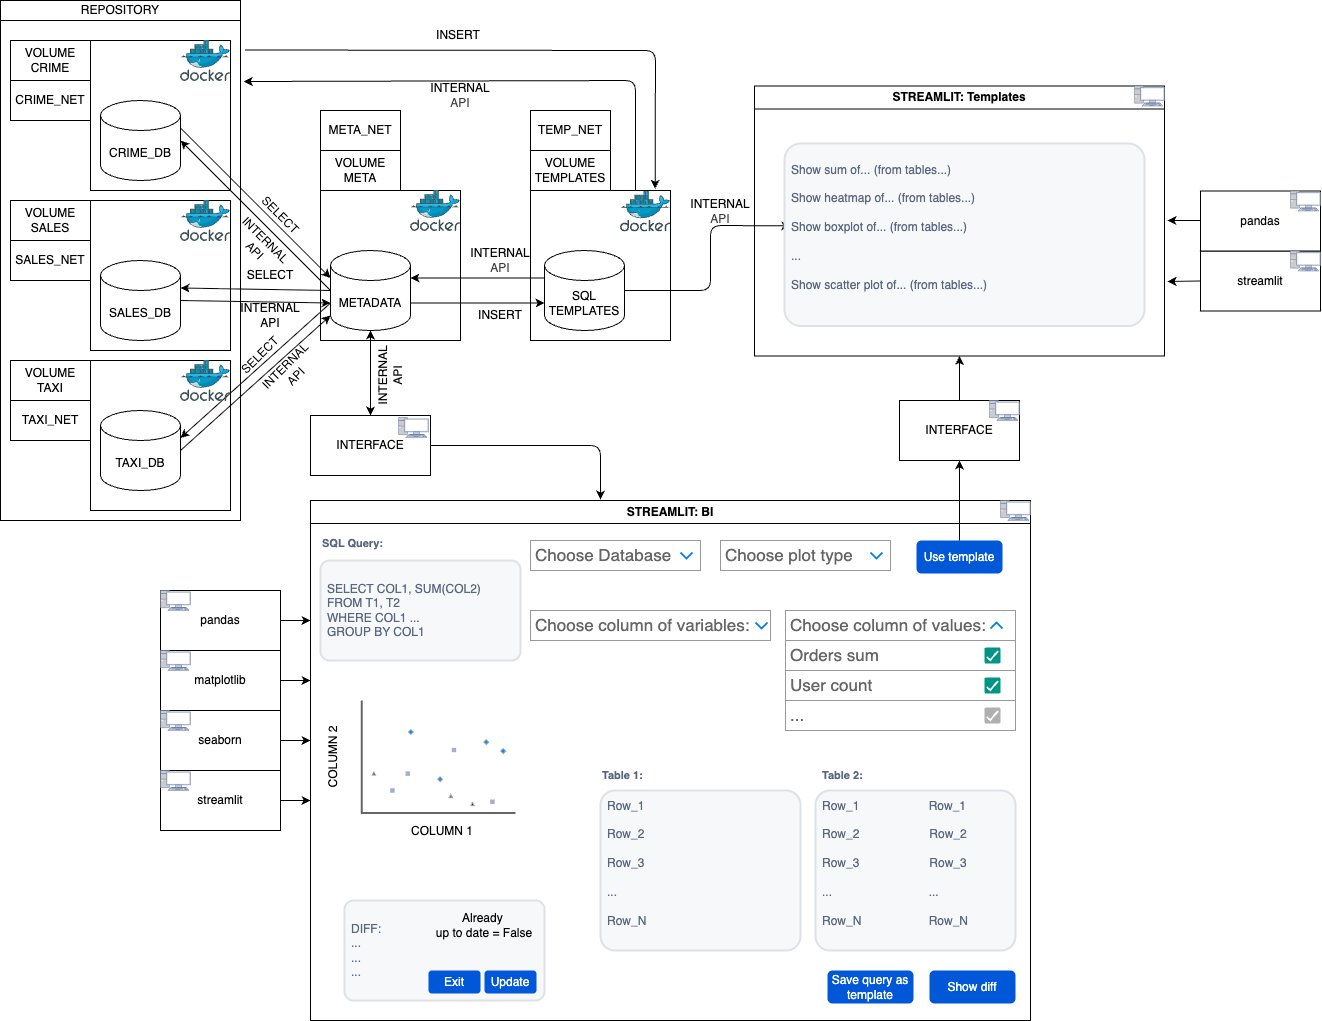
\includegraphics[width=0.7\linewidth]{../schema/l1.png}
    \caption{Архитектура задачи}
    \label{fig:task_arch}
\end{figure}

Далее описываются архитектуры баз данных источников и визуализация архитектур.

\newpage
\section{Базы-источники}
\subsection{База данных: Учет репетиторов для школьников}

Предметная область - репетиторство, то есть индивидуальное или групповое обучение школьников, цель которого углубить знания по предмету,
подготовиться к экзаменам или улучшить успеваемость. Репетитора, как правило, ищет родитель, когда понимает, что ребенку нужны дополнительные занятия.
Занятия проходят в одном из форматов: очно, дистанционно (Zoom, Skype, Telegram и др.) или смешанно. После занятий родитель оставляет отзыв о репетиторе,
а репетитор - отзыв об ученике. Цели базы данных: поиск репетитора, рейтинг и отзывы о репетиторах и учениках, оценка востребованности преподавателей.
Данные сгенерированы: около 300 000 занятий, 40 000 родителей, 4 000 репетиторов и по 60 000 отзывов каждого вида.

Схема extra\_for\_students включает двенадцать таблиц.
Таблица gender - справочник полов. Атрибуты: gender\_id - идентификатор, gender\_name - название.
Таблица city - справочник городов. Атрибуты: city\_id - идентификатор, city\_name - название города, timezone - часовой пояс.
Таблица format - формат занятия (очно, дистанционно, смешанный). Атрибуты: format\_id - идентификатор, format\_name - название формата.
Таблица subjects - справочник школьных предметов. Атрибуты: subject\_id - идентификатор, subject\_name - название предмета.

Таблица parent хранит родителей учеников. Атрибуты: parent\_id - идентификатор, last\_name, first\_name, middle\_name - фамилия, имя и отчество, contact - контакт для связи.
Таблица tutors хранит репетиторов. Атрибуты: tutor\_id - идентификатор, last\_name, first\_name, middle\_name - ФИО, gender\_id - ссылка на пол, city\_id - ссылка на город,
age - возраст (от 18 до 80 лет), experience - опыт преподавания в годах, contact - контакт. Связи N:1 с gender и city.
Таблица learner хранит учеников. Атрибуты: learner\_id - идентификатор, parent\_id - ссылка на родителя, city\_id - ссылка на город, last\_name, first\_name, middle\_name - ФИО,
study\_goal - цель занятий, class - класс (от 1 до 11). Связь N:1 с parent: у одного родителя может быть несколько детей.

Таблица tutor\_subject реализует связь N:N между tutors и subjects (какие предметы преподает репетитор) через составной первичный ключ (tutor\_id, subject\_id).
Таблица learner\_subjects аналогично реализует связь N:N между learner и subjects (по каким предметам занимается ученик), ключ (learner\_id, subject\_id).

Таблица lesson - центральная таблица фактов, содержащая около 300 000 записей. Атрибуты: lesson\_id - идентификатор занятия, subject\_id - ссылка на предмет,
format\_id - ссылка на формат, learner\_id - ссылка на ученика, tutor\_id - ссылка на репетитора, lesson\_date - дата занятия, cost - стоимость в рублях, duration - длительность в минутах.
Таблица review\_of\_tutor хранит отзывы родителей о репетиторе своего ребенка. Атрибуты: review\_id - идентификатор, learner\_id, parent\_id, tutor\_id - ссылки на ученика, родителя и репетитора,
review\_date - дата отзыва, rating - оценка от 1 до 5, review\_text - текст отзыва.
Таблица review\_of\_learner хранит отзывы репетитора об ученике. Атрибуты: review\_id - идентификатор, tutor\_id, learner\_id - ссылки на репетитора и ученика,
review\_date - дата, rating - оценка от 1 до 5, review\_text - текст отзыва.

Ниже на рисунке \ref{fig:extradb}, показана схема базы данных:

\begin{figure}[H]
    \center
    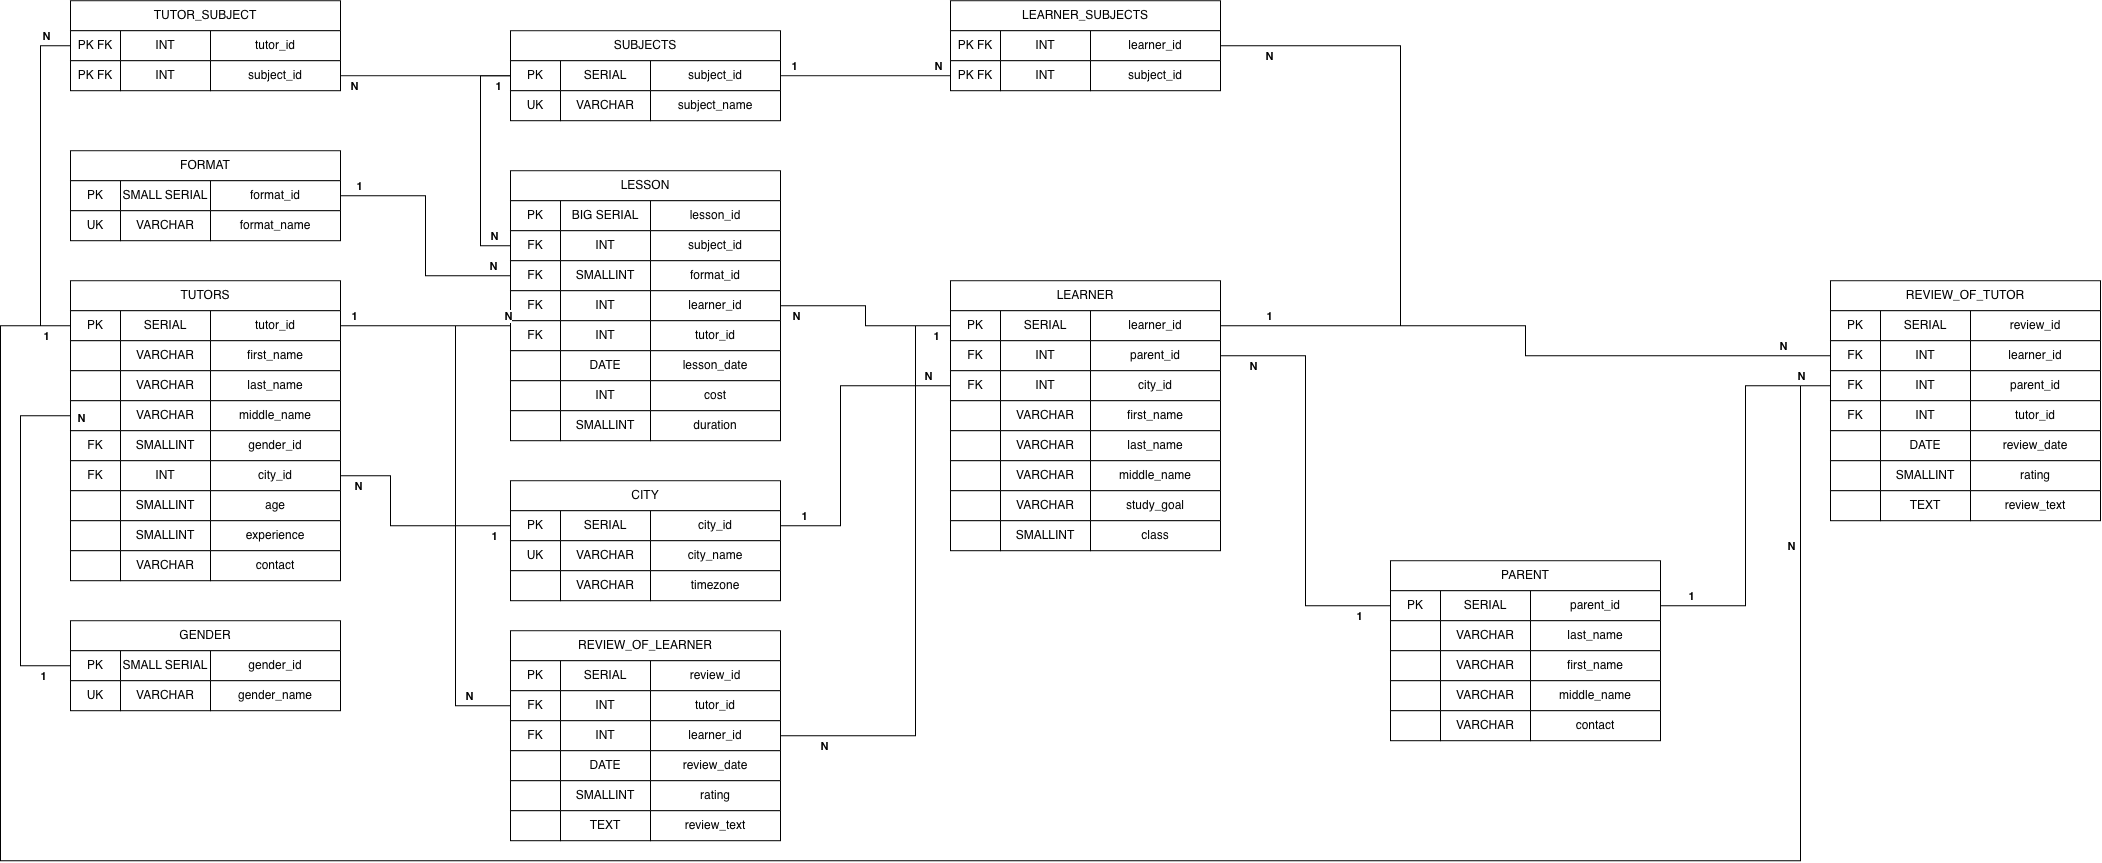
\includegraphics[width=\linewidth]{../schema/db-schema/extra-db/extra-db.png}
    \caption{Архитектура базы данных учета репетиторов}
    \label{fig:extradb}
\end{figure}


\subsection{База данных: Всероссийские соревнования по горнолыжному спорту}

Предметная область - всероссийские соревнования по горнолыжному спорту. Горнолыжный спорт включает пять дисциплин: слалом, гигантский слалом,
супергигант, скоростной спуск и комбинацию. Спортсмены выступают за команды (сборные городов и регионов), старты проходят на горнолыжных курортах,
за соблюдением правил следят судьи. В технических дисциплинах выполняется две попытки, во вторую проходят 30 лучших по первой, итоговое время
складывается из двух попыток. Спортсмен может не финишировать (DNF), быть дисквалифицирован (DSQ) или не стартовать (DNS).
Цели базы данных: личный и командный рейтинг за сезон, места участников, подбор места проведения по погодным условиям.
Данные сгенерированы: 6 000 спортсменов, 4 500 стартов и около 190 000 результатов.

Схема mountain\_sport включает восемь таблиц.
Таблица team хранит команды. Атрибуты: team\_id - идентификатор, team\_name - название команды.
Таблица athlete хранит спортсменов. Атрибуты: athlete\_id - идентификатор, first\_name, last\_name - имя и фамилия, birth\_date - дата рождения,
gender - пол (M или F), team\_id - ссылка на команду. Связь N:1 с team: в команде состоит несколько спортсменов.
Таблица venue хранит горнолыжные курорты и трассы. Атрибуты: venue\_id - идентификатор, venue\_name - название, winter\_weather\_conditions и spring\_weather\_conditions - погодные условия зимой и весной.
Таблица judge хранит главных судей соревнований. Атрибуты: judge\_id - идентификатор, last\_name, first\_name - фамилия и имя.

Таблица competition хранит старты. Атрибуты: competition\_id - идентификатор, competition\_name - название, discipline - дисциплина, competition\_date - дата,
attempt1\_result и attempt2\_result - лучшее время первой и второй попытки на старте в секундах, venue\_id - ссылка на место проведения, judge\_id - ссылка на главного судью. Связи N:1 с venue и judge.
Таблица athlete\_competition реализует связь N:N между athlete и competition (заявка спортсмена на старт). Атрибуты: athlete\_competition\_id - идентификатор, athlete\_id, competition\_id - ссылки,
на пару (athlete\_id, competition\_id) установлено уникальное ограничение.
Таблица attempt - справочник итогов выступления. Атрибуты: attempt\_id - идентификатор, attempt\_status - статус (финишировал, DNF, DSQ, DNS).

Таблица result - центральная таблица фактов, содержащая около 190 000 записей. Атрибуты: result\_id - идентификатор, athlete\_id - ссылка на спортсмена, competition\_id - ссылка на старт,
attempt1\_result и attempt2\_result - время первой и второй попытки в секундах (NULL, если спортсмен не финишировал или не прошел во вторую попытку), attempt\_id - ссылка на итог выступления.
Спортсмен имеет не более одного результата на старте, что обеспечивается уникальным ограничением (athlete\_id, competition\_id).

Далее показана схема базы данных горнолыжных соревнований \ref{fig:mountaindb}:
\begin{figure}[H]
    \center
    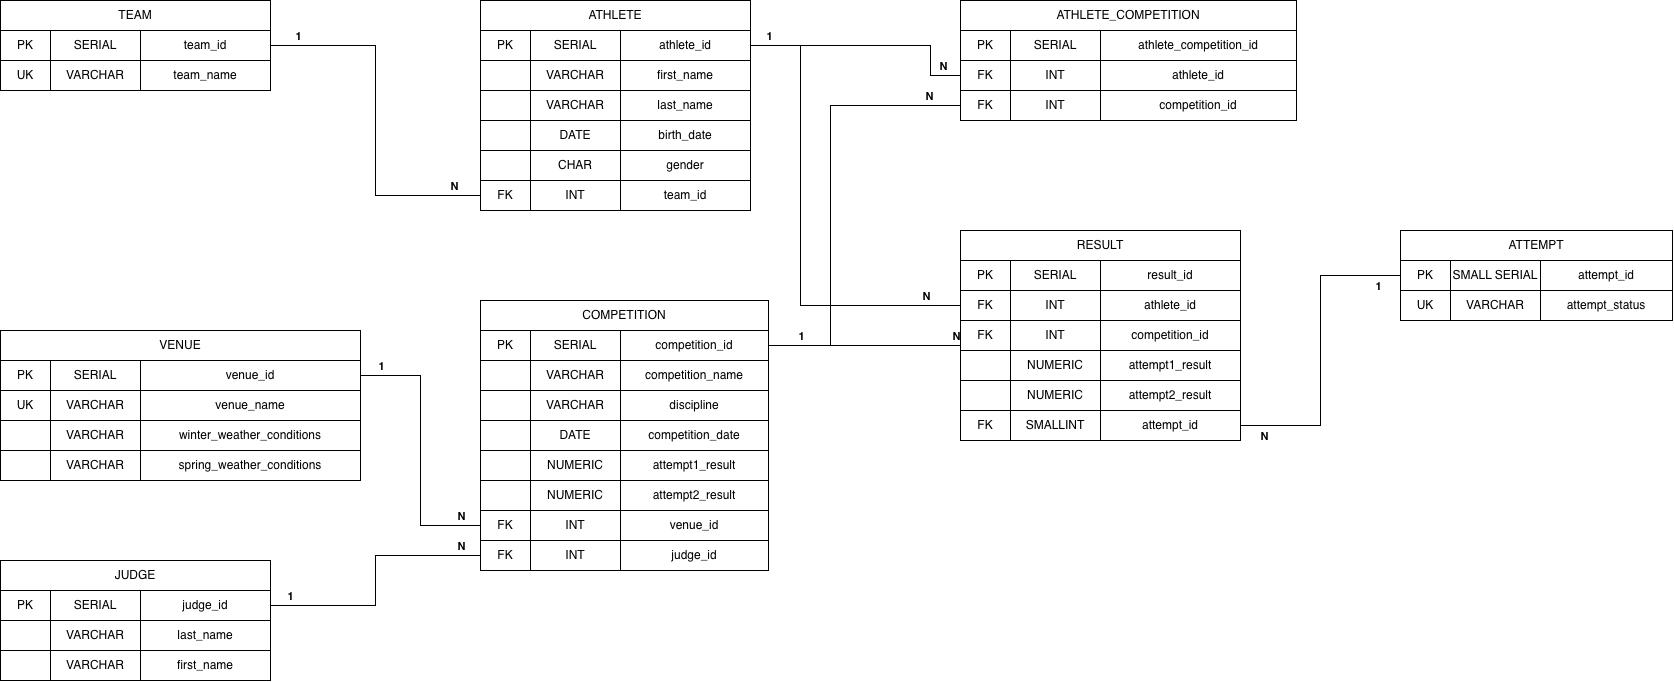
\includegraphics[width=\linewidth]{../schema/db-schema/mountain-db/mountain-db.png}
    \caption{Архитектура базы данных горнолыжных соревнований}
    \label{fig:mountaindb}
\end{figure}

\subsection{База данных: Спортсмены и соревнования в чирлидинге}

Предметная область - чир спорт, сочетающий элементы танцев, гимнастики и акробатики. Спортсмены состоят в клубах, клубы относятся к региональным федерациям,
регионы к странам. Спортсмены выполняют разряды, от юношеских до КМС и мастера спорта, разряд подтверждается на официальных соревнованиях и оценивается судейской бригадой.
Соревнования бывают разного уровня (городские, региональные, всероссийские, международные), выступления проходят в номинациях (чир-данс, чир-микс, фристайл, группа, двойка, соло)
и возрастных категориях. Выступления оценивает судейская бригада, максимальный балл - 100, за нарушения выставляются сбавки, возможна дисквалификация.
Цели базы данных: оценка выступлений судьями, учет спортсменов, определение лучших спортсменов, клубов и регионов, формирование цифрового паспорта спортсмена.
Данные сгенерированы: 60 000 спортсменов, 1 200 клубов, 1 200 соревнований, 2 000 судей и не менее 300 000 записей участия спортсменов в выступлениях.

Схема sport\_and\_cheerleaders включает шестнадцать таблиц.
Таблица country - справочник стран. Атрибуты: country\_id - идентификатор, country - название страны.
Таблица region хранит регионы. Атрибуты: region\_id - идентификатор, region\_name - название, region\_ranking - место региона в рейтинге, sportsmans\_count - количество спортсменов,
country - ссылка на страну. Связь N:1 с country, пара (country, region\_name) уникальна.
Таблица club хранит клубы. Атрибуты: club\_id - идентификатор, club\_name - название, club\_ranking - место в рейтинге, region\_id - ссылка на регион, birthdate - дата основания, email - почта клуба.

Таблица grade\_type - справочник разрядов и званий (юношеские, 1--3 разряд, КМС, МС, МСМК). Атрибуты: grade\_type\_id - идентификатор, grade\_type - название.
Таблица competition\_type - справочник уровней соревнований. Атрибуты: competition\_type\_id - идентификатор, competition\_type - название уровня.
Таблица grade хранит приказы о присвоении разряда. Атрибуты: grade\_id - идентификатор, grade\_type - ссылка на разряд, date - дата присвоения,
competition\_type - ссылка на уровень соревнований, на котором выполнен разряд, verification - подтвержден ли разряд федерацией.
Таблица sportsman хранит спортсменов. Атрибуты: sportsman\_id - идентификатор, sportsman\_name, sportsman\_lastname, sportsman\_middlename - имя, фамилия и отчество,
grade\_id - ссылка на приказ о разряде (NULL, если разряда нет), club\_id - ссылка на клуб, sportsman\_birthdate - дата рождения.

Таблица location - справочник мест проведения. Атрибуты: location\_id - идентификатор, location - адрес площадки.
Таблица competition хранит соревнования. Атрибуты: competition\_id - идентификатор, competition\_name - название, competition\_date - дата,
competition\_type - ссылка на уровень, location - ссылка на место проведения.
Таблица perfomance\_type - справочник номинаций. Атрибуты: perfomance\_type\_id - идентификатор, perfomance\_type - название номинации.
Таблица age\_category - справочник возрастных категорий. Атрибуты: age\_category\_id - идентификатор, age\_category - название категории.

Таблица judge\_type - справочник ролей судей (главный судья, судья по технике, по артистизму, по сложности). Атрибуты: judge\_type\_id - идентификатор, judge\_type - название роли.
Таблица judge хранит судей. Атрибуты: judge\_id - идентификатор, judge\_name, judge\_lastname, judge\_middlename - ФИО, judge\_type - ссылка на роль, judge\_score - квалификационный балл судьи (от 0 до 100).
Таблица judge\_panel хранит судейские бригады. Атрибуты: judge\_panel\_id - идентификатор, judge\_count - число судей, disqualification - была ли вынесена дисквалификация,
total\_score - сумма выставленных баллов, total\_allowance - сумма сбавок.
Таблица judge\_panel\_judge реализует связь N:N между judge\_panel и judge (состав бригады). Атрибуты: judge\_panel\_judge\_id - идентификатор, judge\_panel\_id, judge\_id - ссылки.

Таблица perfomance хранит выступления. Атрибуты: perfomance\_id - идентификатор, competition\_id - ссылка на соревнование, perfomance\_place - занятое место (NULL при дисквалификации),
perfomance\_type - ссылка на номинацию, sportsman\_count - число спортсменов в составе, age\_category - ссылка на возрастную категорию, judge\_panel - ссылка на судейскую бригаду.
Таблица sportsman\_perfomance - центральная таблица фактов, реализующая связь N:N между sportsman и perfomance (состав выступления), содержит не менее 300 000 записей.
Атрибуты: perfomance\_sportsman\_id - идентификатор, perfomance\_id, sportsman\_id - ссылки, пара (perfomance\_id, sportsman\_id) уникальна.

На рисунке \ref{fig:sportdb} показана схема базы данных чирлидинга:
\begin{figure}[H]
    \center
    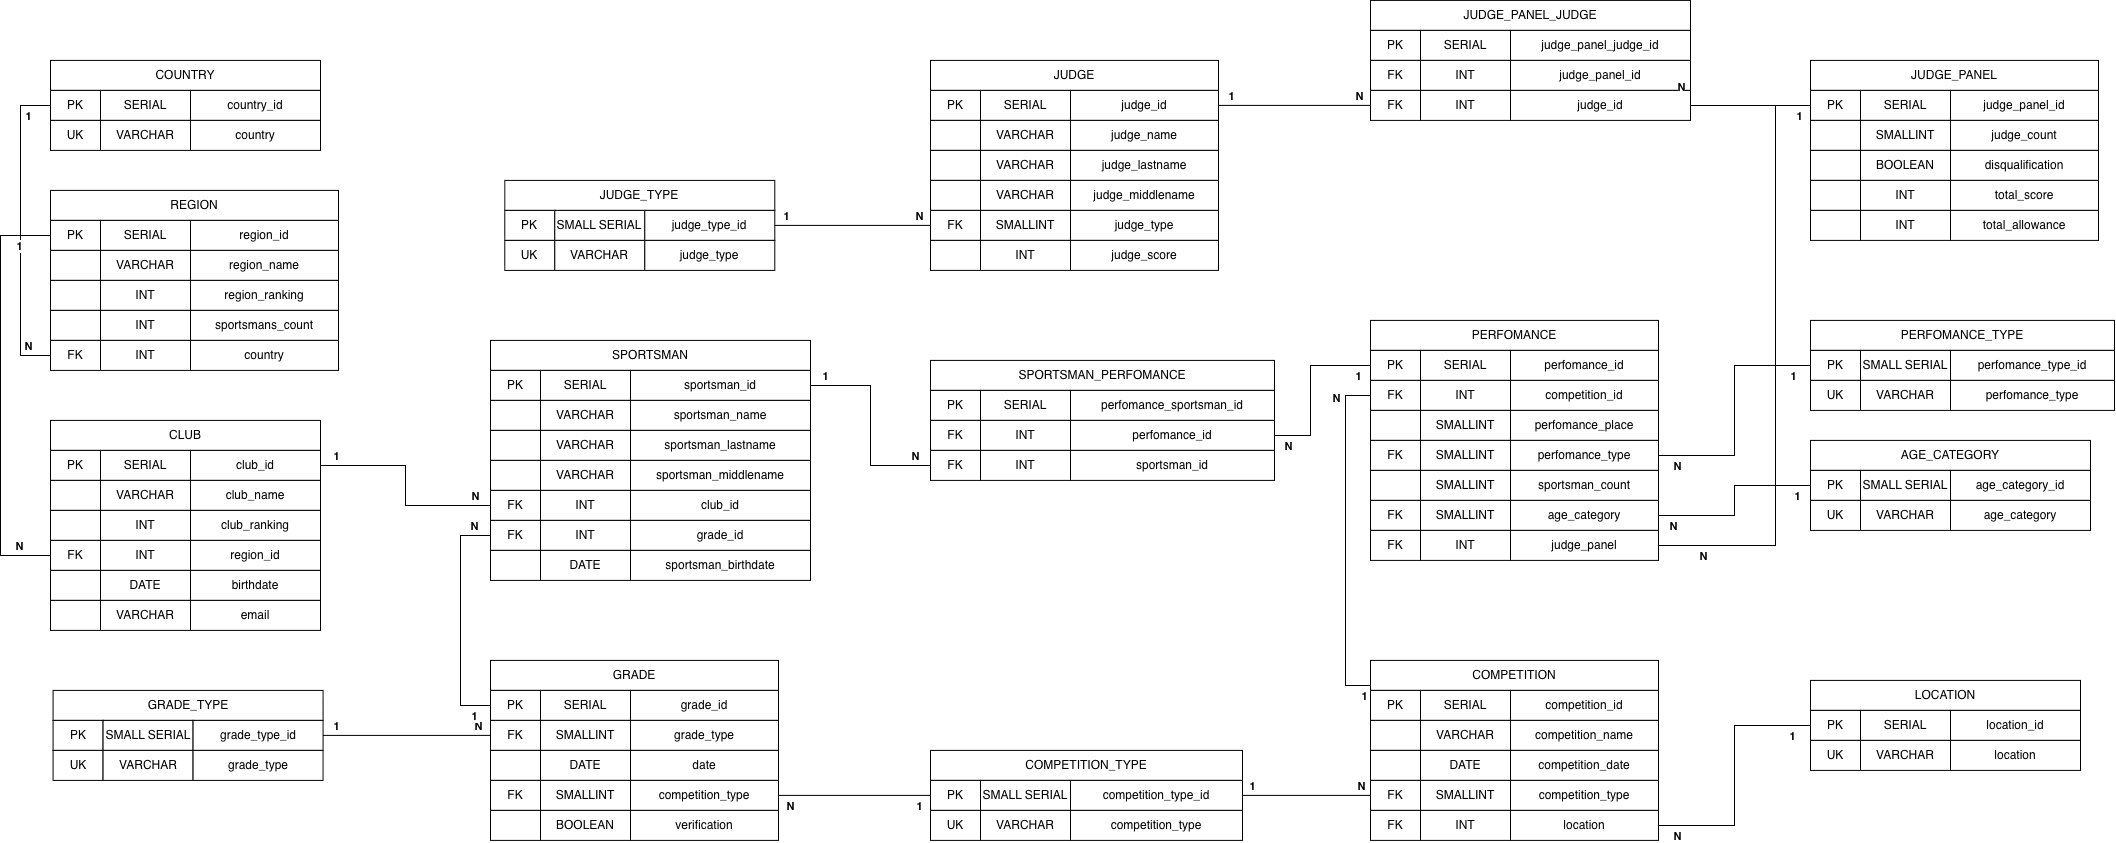
\includegraphics[width=\linewidth]{../schema/db-schema/sport-db/sport-db.png}
    \caption{Архитектура базы данных спортсменов и соревнований в чирлидинге}
    \label{fig:sportdb}
\end{figure}

\section{Проектирование информационной схемы}

На рисунке \ref{fig:metadb}, представлена схема базы данных имплементирующую логику денормализованной информационной схемы. 

\begin{figure}[H]
    \center
    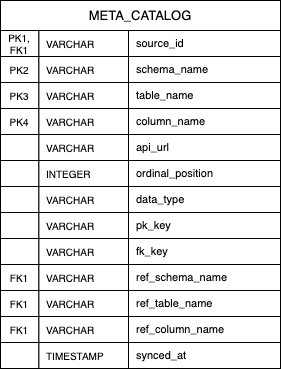
\includegraphics[width=0.4\linewidth]{../schema/db-schema/meta-db/meta-db.png}
    \caption{Архитектура базы метаданных}
    \label{fig:metadb}
\end{figure}

Тут, таблица meta.catalog - это аналог информационной схемы, в которой каждая строка это одна колонка источника. 
Это было сделано для того, что бы в последующих шаблонных запросах не использовать JOIN механизм: вся информация о колонке, ее таблице, источнике и связях лежит в одной строке. 
Таблица разделена на несколько уровней.

Уровень источника:
\begin{itemize}
    \item source\_id - идентификатор источника (одна из трех баз). Нужен, что бы отличать одинаковые по имени таблицы из разных источников, 
    и по нему же строится ссылка на meta.sources, где хранятся адреса баз данных источников;
    \item api\_url - адрес REST-агента источника. Хранится прямо в строке каталога, что бы по выбранной колонке сразу знать, 
    к какому агенту отправлять запрос, без обращения к другой таблице.
\end{itemize}

Уровень таблицы:
\begin{itemize}
    \item schema\_name - имя схемы в БД источника. Нужно, так как в разных схемах могут быть таблицы с одинаковым именем;
    \item table\_name - имя таблицы в БД источника. Вместе с schema\_name используется в блоке FROM генерируемого SQL-запроса.
\end{itemize}

Уровень колонки:
\begin{itemize}
    \item column\_name - имя самой колонки. Используется в SELECT, WHERE, GROUP BY генерируемого запроса и как подпись в интерфейсе;
    \item ordinal\_position - порядковый номер колонки в исходной таблице. Позволяет выводить колонки в интерфейсе в том же порядке, что и в источнике, 
    а так же участвует в сравнении структур (Show diff): если порядок колонок изменился, это будет видно как отличие;
    \item data\_type - тип данных колонки в источнике. Тип определяет, что можно делать с колонкой: числовые колонки подходят для агрегатных функций (SUM, AVG) и оси значений графика, 
    даты и время для оси времени, строковые для группировки и фильтров с текстовыми операторами. Так же тип сравнивается при Show diff.
\end{itemize}

Уровень ключей (описание связей):
\begin{itemize}
    \item pk\_key - признак первичного ключа. Значение PK ставится, если ключ таблицы одиночный. Если ключ составной, то колонки нумеруются: PK1, PK2, ... 
    Номер это позиция колонки в составном ключе. Он нужен, что бы понимать, какие колонки вместе однозначно определяют строку и в каком порядке идут. 
    Если NULL, колонка не входит в первичный ключ;
    \item fk\_key - номер внешнего ключа в таблице: FK1, FK2, ... Номер отличает один внешний ключ таблицы от другого: если таблица ссылается на две разные таблицы, 
    то это будут FK1 и FK2. Колонки составного внешнего ключа получают один и тот же номер, по нему видно, что их нужно соединять вместе. 
    Если NULL, колонка не является внешним ключом;
    \item ref\_schema\_name, ref\_table\_name, ref\_column\_name - на какую схему, таблицу и колонку ссылается внешний ключ. Заполняются только вместе с fk\_key (это проверяется ограничением CHECK). 
    По ним система находит, какие таблицы можно соединять между собой, и строит JOIN в запросе автоматически, а не заставляет пользователя выбирать его вручную.
\end{itemize}

Служебное поле: synced\_at - время последней синхронизации строки с источником. Показывает, насколько актуален каталог, 
и обновляется при синхронизации, если структура таблицы в источнике отличается от сохраненной.

Первичным ключом таблицы является составной ключ (source\_id, schema\_name, table\_name, column\_name), так как этого набора достаточно, что бы однозначно определить колонку среди всех источников. 
Внешний ключ ссылается на саму таблицу (ref\_* колонки указывают на строку каталога с тем же source\_id), 
поэтому связи между таблицами хранятся внутри каталога.

Еще нужны ограничения таблицы, что бы каталог оставался согласованным:
\begin{itemize}
    \item pk\_catalog - составной первичный ключ, не дает добавить одну и ту же колонку источника дважды при синхронизации;
    \item fk\_catalog\_ref - внешний ключ на саму таблицу, гарантирует, что ссылка ref\_* указывает на реально существующую колонку каталога. 
    ON DELETE CASCADE удаляет связи вместе с удаленной колонкой, что бы не оставалось ссылок в никуда.
    \item ck\_catalog\_pk\_key и ck\_catalog\_fk\_key - проверяют формат значений (PK, PK1, PK2, ... и FK1, FK2, ...), что бы по ним можно было разбирать номер ключа;
    \item ck\_catalog\_fk\_ref - поля fk\_key и ref\_* должны быть либо все пустыми, либо все заполненными. Это исключает \guillemetleft неполный\guillemetright внешний ключ, по которому нельзя построить JOIN.
\end{itemize}

\newpage
\section{Проектирование базы данных шаблонов}

База данных предназначена для хранения шаблонов SQL-запросов, используемых в пользовательском интерфейсе системы. Схема содержит единственную таблицу form\_templates, 
реализующую денормализованную структуру для хранения готовых запросов и параметров формы визуализации. 

Атрибуты таблицы: 
\begin{itemize}
    \item template\_id - первичный ключ таблицы;
    \item template\_name - уникальное имя шаблона, что бы в интерфейсе можно было назвать или выбрать; 
    \item sql\_text - сам SQL запрос;
    \item source\_id - идентификатор базы данных источника;
    \item schema\_name - имя схемы в базе источнике 
    \item dimension\_col - имя категориальной переменой что б понимать какую колонку выбирать;
    \item measure\_col - имя значений, так же что б понимать какую колонку выбрать;
    \item second\_dim - имя вторыйх значений если будет возможность создать heatmap; 
    \item agg\_func - выбор аггрегатной функции (только SUM, COUNT);
    \item row\_limit - ограничение на количество строк (для LIMIT);
    \item created\_at - дата и время создания шаблона;
    \item last\_used\_at - дата последнего использования, так как планируется удалять шаблон если не используется более 10 дней. 
\end{itemize}

Денормализованная структура таблицы позволяет восстанавливать параметры формы интерфейса из сохраненного шаблона без дополнительных соединений.

Сама схема преведена в рисунке \ref{fig:template}:

\begin{figure}[H]
    \center
    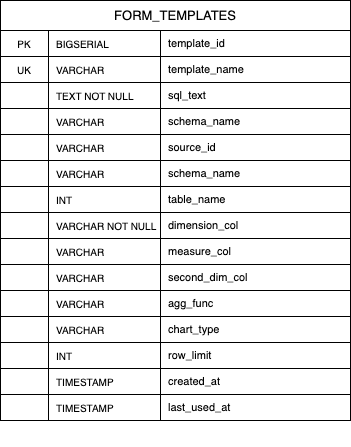
\includegraphics[width=0.4\linewidth]{../schema/db-schema/template-db.png}
    \caption{Архитектура базы шаблонов}
    \label{fig:template}
\end{figure}

\newpage
\section{Контейнеризация}
Для развертывания системы используется Docker, которая даст изоляцию компонентов приложения. То есть позволит сделать все базы независимыми.
Каждая база данных запускается в отдельном контейнере на основе образа postgres16 Alpine. 

В составе системы пять независимых контейнеров postgres: 

\begin{itemize}
    \item extra\_db - база данных учета репетиторов для школьников;
    \item mountain\_db - база данных соревнований по горнолыжному спорту;
    \item sport\_db - база данных спортсменов и соревнований в чирлидинге;
    \item meta\_db - база данных метаданных;
    \item templates\_db - база данных шаблонов SQL запросов.
\end{itemize}

Каждый контейнер представляет собой самостоятельный экземпляр postgres со своей базой данных, пользователем, паролем, каталогом хранения и сетевой конфигурацией. 
Такое разделение препятствует непосредственному объединению баз данных на уровне СУБД и обеспечивает независимость источников. 
Взаимодействие между компонентами системы выполняется с помощью подключения одной базы данных к другой через REST API.

Конфигурация каждого контейнера задается с помощью файла Docker Compose. Для всех экземпляров postgres используются следующие параметры:

\begin{itemize}
\item image - образ postgres версии 16 на базе Alpine Linux;
\item container\_name - фиксированное имя контейнера;
\item restart: unless-stopped - автоматический перезапуск контейнера после сбоя или перезапуска Docker;
\item environment - параметры инициализации базы данных;
\item volumes - подключение постоянного хранилища и каталога начальной инициализации;
\item networks - подключение контейнера к выделенной изолированной сети;
\item healthcheck - проверка доступности postgres.
\end{itemize}

Параметр postgres\_DB - задает имя базы данных при первом запуске контейнера, (postgres\_USER, postgres\_PASSWORD) - учетная запись пользователя.
Для каждой БД создается отдельное значение (например для БД репетиторов - extra\_user, extra\_pass). 


    \subsection{Тома}
    Для сохранения данных postgres используются именованные Docker-тома. Каждая база данных имеет собственный том, не используемый другими контейнерами.
    Каждый том подключается к каталогу /var/lib/postgres/data соответствующего контейнера. Фактическое размещение кластера postgres определяется параметром PGDATA, имеющим значение /var/lib/postgres/data/pgdata.

    Использование отдельных именованных томов обеспечивает сохранность данных при удалении или пересоздании контейнеров.
    \subsection{Сети}
    Для каждой базы данных создается отдельная изолированная сеть Docker. В каждую сеть подключается только один контейнер postgres. То есть базы данных источников не имеют прямого сетевого доступа
    друг к другу и не могут выполнять непосредственные межбазовые SQL-запросы.

    Обмен данными между базами данных, базой метаданных, базой шаблонов и пользовательским интерфейсом осуществляется через REST API. 
    Сетевая изоляция обеспечивает независимость источников и ограничивает прямое взаимодействие между контейнерами.

    \subsection{Порты}
    Внутри всех контейнеров postgres используется стандартный порт: 5432. Для доступа с хостовой системы каждому контейнеру назначается отдельный внешний порт:

    \begin{table}[H]
        \centering
        \caption{Распределение портов}
        \label{tab:ports}
        \begin{tabular}{|l|l|l|}
            \hline
            Контейнер & Внутренний порт & Внешний порт \\
            \hline
            \texttt{templates\_db} & 5432 & 5436 \\
            \hline
            \texttt{meta\_db} & 5432 & 5437 \\
            \hline
            \texttt{extra\_db} & 5432 & 5438 \\
            \hline
            \texttt{mountain\_db} & 5432 & 5439 \\
            \hline
            \texttt{sport\_db} & 5432 & 5440 \\
            \hline
        \end{tabular}
    \end{table}

Проброс портов выполняется по схеме:

$$
    ExternalPort:5432
$$

То есть например 5438:5432 означает, что подключения к порту 5438 хостовой системы перенаправляются на порт 
5432 postgres внутри контейнера базы источника.

\newpage
\section{Разработка системы}
    % Про проектирование, psycopg
Слой доступа к данным вынесен в отдельный модуль и построен так, что Python отвечает только за подстановку имен и вывод,
а вся работа с данными остается на стороне СУБД. Для связи с postgres используется драйвер psycopg третьей версии,
так как с его помощью в дальнейшем данные можно будет легко переводить в массивы для построения графиков.
Модуль разбит на три части: соединение и чтение окружения, текстовые шаблоны запросов, перевод результата в массивы.

    \subsection{Соединение}
    % про то как подключаемся к контейнерам
Каждая база живет в своем контейнере, наружу проброшен только порт postgres, поэтому с точки зрения слоя доступа
подключение ничем не отличается от обычного локального: адрес, порт, имя базы, пользователь и пароль.
Соединение открывается на время одного запроса и закрывается контекстным менеджером.

\begin{lstlisting}[language=Python, caption={Чтение каталога метаданных}, label={lis:catalog_read}]
def catalog(source_id):
    with psycopg.connect(row_factory=dict_row, **meta()) as connection:
        with connection.cursor() as cursor:
            cursor.execute(template.CATALOG_SQL, (source_id,))
            return cursor.fetchall()
\end{lstlisting}

Ошибки драйвера перехватываются и возвращаются текстом, то есть
недоступная база или неверное имя колонки приводят к выводу сообщения, после 
чего запрос о вводе имени повторяестя.

    \subsection{Окружение}
    % про .env и что за секреты (не все просто сгруппировать типа DB_NAME,...)
Все параметры подключения собраны в одном файле credentials.env. 

Переменные сгруппированы по префиксу источника, для каждой базы задаются хост, порт, имя, пользователь, пароль и образ.
Слой доступа разбирает файл сам и собирает словарь источников по суффиксу имени переменной: встретив ключ,
оканчивающийся на DB\_NAME, он достает по тому же префиксу остальные параметры. Благодаря этому добавление
еще одной базы не требует правок кода, достаточно дописать блок переменных.

    \subsection{Передача данных}
    % про то как контейнеры общаются между собой и интерфейсом локально
Данные и метаданные приходят из разных баз. Сначала выполняется запрос к базе метаданных, откуда берется описание
выбранного источника, затем по этому описанию собирается запрос и отправляется уже в саму базу-источник.
Такое разделение и позволяет системе оставаться независимой от источников.

Передаются при этом текст запроса в одну сторону и результат в другую. Рядом с каждой базой
поднят свой REST, который принимает запрос методом POST, выполняет его и возвращает ответ в формате JSON
из списка имен колонок и списка строк. Отдельным методом агент отдает описание своих таблиц и колонок,
откуда база метаданных и наполняет каталог.

    \subsection{Шаблонный запрос}
    % как проектируется (с помощью чего, почему именно так) - как именно работает с другими БД источниками и мета данными
Запрос к источнику описан одной строкой-шаблоном с именованными
местами подстановки:

\begin{lstlisting}[language=SQL, caption={Шаблон запроса к источнику}, label={lis:query_template}]
SELECT {group_cols}, {agg_func}({agg_arg}) AS value
FROM {table}
GROUP BY {group_cols}
ORDER BY value DESC
LIMIT 20
\end{lstlisting}

Подстановка текстовая так как таблицу или колонку так передать нельзя.
 Чтобы подстановка не давала ошибок
каждое имя перед этим проверяется по каталогу метаданных, и в шаблон попадает только то, что там найдено.

Полное имя собирается из полей schema\_name и table\_name строки каталога:

\begin{lstlisting}[language=SQL, caption={Запрос к каталогу метаданных}, label={lis:catalog_sql}]
SELECT schema_name, table_name, column_name, data_type,
       pk_key, fk_key, ref_table_name, ref_column_name
FROM meta.catalog
WHERE source_id = %s
ORDER BY table_name, ordinal_position
\end{lstlisting}

Порядок строк каталога совпадает с порядком колонок в исходной таблице, что позволяет показывать атрибуты так,
как они объявлены в источнике. Поля ключей и ссылок в текущем варианте шаблона
не участвуют в сборке, но читаются вместе с остальными, так как описывают связи источника и нужны при расширении
запроса на несколько таблиц.

        \subsubsection{Агрегатные функции}
        % как интегрируем какие можно выбрать (count, sum) - как именно работает с другими БД источниками и мета данными
Допустимых функций пока две, SUM и COUNT,
и выбор ограничен списком, то есть в шаблон не может попасть произвольное слово.

Аргументом служит колонка значений, выбранная пользователем и проверенная по каталогу. Если колонка не задана,
агрегат вырождается в COUNT по всем строкам, и вместо имени подставляется звездочка. 
То есть когда суммировать нечего, считается количество записей.

Тип колонки при этом берется из поля data\_type каталога, то есть система знает, что числовое, а что нет,
не обращаясь к самому источнику.

        \subsubsection{Условие}
        % как интегрируем WHERE (что можно ставить)(пропустить) - как именно работает с другими БД источниками и мета данными
        \subsubsection{Ограничение по строкам}
        % как интегрируем LIMIT (пропустить) - как именно работает с другими БД источниками и мета данными
        \subsubsection{Группировка}
        % как определяется как интегрируется как работает (в приложении) - как именно работает с другими БД источниками и мета данными
Группировка определяется набором выбранных атрибутов. 
Основная категориальная колонка плюс дополнительные, если они заданы.
Этот набор подставляется в шаблон дважды, в список выборки и в GROUP BY, из одного и того же места, поэтому запрос
не может оказаться несогласованным, когда колонка выбирается, но не группируется.

Результат агрегата всегда получает фиксированное имя value и по нему же сортируется по убыванию. Фиксированное имя
избавляет последующую обработку от разбора заголовков. То есть последняя колонка результата это значение,
а все предыдущие это подписи.

    \subsection{Сохранение шаблонов запросов}
    % пропустить

    \subsection{Перевод в NumPy массив}
    % как получаем данные, как переводим их (переход к тому что они нужны для matplotlib, seaborn - пропусти только matplotlib)
Курсор возвращает результат в виде списка кортежей и отдельного списка имен колонок для вывода таблиц.
А для построения графика данные нужно разложить на две однотипные последовательности.
Последняя колонка это агрегат, остальные это подписи. Подписи склеиваются
в строку, значения приводятся к числу с плавающей точкой, после чего обе последовательности оборачиваются в массивы NumPy:

\begin{lstlisting}[language=Python, caption={Перевод результата в массивы}, label={lis:to_arrays}]
def to_arrays(rows):
    labels = np.array([" ".join(str(cell) for cell in row[:-1]) for row in rows])
    values = np.array([float(row[-1]) for row in rows])
    return labels, values
\end{lstlisting}

Перевод к float так как в postgres numeric драйвер отдает как Decimal,
с которым графические библиотеки работать не будут. Массивы NumPy выбраны потому, что именно их принимают функции
построения графиков, и потому что индексация массива позволяет задать позиции столбцов и точек по оси абсцисс.

    \subsection{Построение графиков}
    % виды (scatter, bar (покачто)), что основная matplotlib , что б визуализировать и т.д
Визуализация построена на matplotlib. Поддерживаются два вида графиков: столбчатый, показывающий соотношение
агрегата между категориями, и точечный, удобный когда хочется посмотреть разброс значений.

По оси абсцисс откладываются порядковые номера, полученные через arange, подписи же
навешиваются на деления отдельно и поворачиваются, иначе длинные категориальные значения накладываются друг на друга.

    \subsection{Запуск}
    % опиши как запускаются контейнеры и приложение 
Каждый контейнер поднимается своим compose-файлом, а параметры подключения берутся из общего файла окружения,
который передается ключом env-file.

\begin{lstlisting}[language=bash, caption={Запуск контейнеров}, label={lis:up}]
docker-compose --env-file credentials.env -f databases/new/extra_for_students/docker-compose.yml up -d
docker-compose --env-file credentials.env -f databases/new/mountain_sport/docker-compose.yml up -d
docker-compose --env-file credentials.env -f databases/new/sport_and_cheerleaders/docker-compose.yml up -d
docker-compose --env-file credentials.env -f information-schema/docker-compose.yml up -d
docker-compose --env-file credentials.env -f templates-db/docker-compose.yml up -d
\end{lstlisting}

Порядок важен - база метаданных подключается к сетям источников как к внешним, поэтому сети
должны быть созданы раньше. Внутри стека порядок обеспечивает сам compose связи стартуют только после того,
как проверка готовности баз прошла успешно. При остановке порядок обратный, иначе Docker не даст удалить
сети источников.

Приложение запускается отдельно, вне Docker, из окружения conda с установленными psycopg, numpy и matplotlib:

\begin{lstlisting}[language=bash, caption={Запуск приложения}, label={lis:run}]
python temp/app.py
\end{lstlisting}

Ниже показан пример сокращенного вывода (см. листинг \ref{lis:example_1}) и ее графика (см. рис. \ref{fig:first_plot}):

\begin{lstlisting}[caption={Пример работы}, label={lis:example_1}]
Which db ? 
    crime
Which table ? 
    incidents
Columns:
    incident_id ... ward community_area year
    Variable ? year
    Values ? ward
    Agg func ? count
    Plot type ? bar    

SELECT crime.incidents.year, COUNT(crime.incidents.ward) AS value
FROM crime.incidents
GROUP BY crime.incidents.year
ORDER BY value DESC
LIMIT 20

year  value
2021  806  
...
2010  438  
\end{lstlisting}

\begin{figure}[H]
    \center
    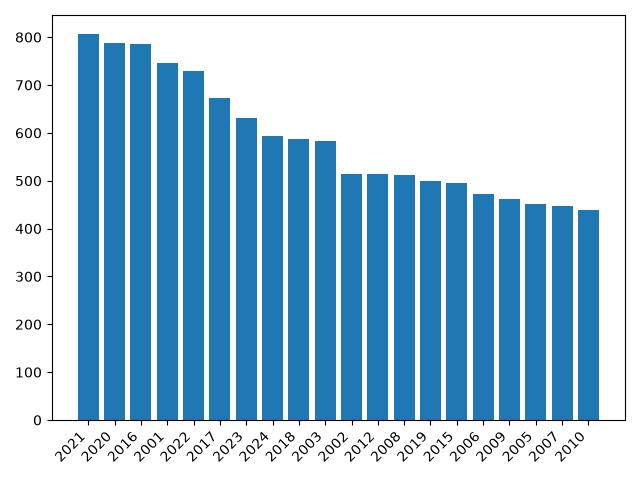
\includegraphics[width=0.6\linewidth]{img/PLOT_EXAMPLE_1.png}
    \caption{Пример вывода графика}
    \label{fig:first_plot}
\end{figure}


\newpage
\section{Интерфейс}
Для создания минимальной версии BI системы, было необходимо разработать 
пользовательский интерфейс включающий в себя: выбор конкретной базы данных источников (или все базы),
выбор таблиц из источников, выбор аггрегатной функции, выбор типа графика, ввод условий, 
ввод количества вывода строк, и вывод основных и дополнительных таблиц.

Интерфейс собран на streamlit и занимает одну страницу, разделенную на две колонки: справа форма с элементами
управления, слева текст собранного запроса и график по нему. Под ними выводятся таблицы с результатом.

    \subsection{Формы}
    % описать формы ввода LIMIT, WHERE, choose database, choose variable table, choose values table 
Основные параметры задаются выпадающими списками, так как все допустимые значения известны заранее из каталога метаданных:
выбор базы данных, выбор таблицы, выбор вида графика, выбор колонки категорий, выбор колонки значений и выбор агрегатной функции.
Список колонок показывает рядом с именем короткое обозначение типа, что бы было понятно, что можно суммировать, а что нет.

Ограничение на количество строк задается текстовым полем.
 Условие отбора вынесено во всплывающую панель, где для каждой колонки стоит выпадающий список
с оператором сравнения и текстовое поле для значения; для строковых колонок оператор не выбирается.

Ниже показаны интерфейсы форм где: 

\begin{itemize}
    \item \textcolor{red}{Красный цвет} - кнопка;
    \item \textcolor{yellow}{Желтный цвет} - выпадающий список;
    \item \textcolor{green}{Зеленый цвет} - статический вывод;
    \item \textcolor{blue}{Синий цвет} - поле ввода.
\end{itemize}

    \subsection{Выбор нескольких колонок}
    % описать формы выбора нескольких таблиц из выпадающего списка 
Отдельная всплывающая панель содержит перечень остальных колонок таблицы, каждая с флажком и подписью типа.
Она нужна, что бы кроме агрегированного результата посмотреть исходные значения: отмеченные колонки выводятся
второй таблицей рядом с основной. На рисунке \ref{fig:additional} показан интерфейс выбора дополнительных колонок.
\begin{figure}[H]
        \center
        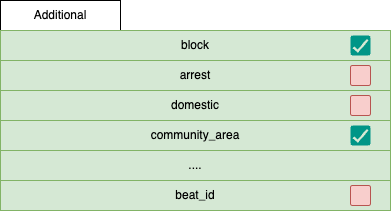
\includegraphics[width=0.4\linewidth]{../interface/ADDITIONAL.png}
        \caption{Интерфейс отличий}
        \label{fig:additional}
\end{figure}

    \subsection{Вывод таблиц}
    % описать вывод таблиц 
Результат показывается табличным блоком с прокруткой и постраничным просмотром: номер страницы задается
числовым полем, под таблицей выводится подпись с диапазоном показанных строк и общим их числом.
Основная и дополнительная таблицы располагаются рядом в двух колонках.

    \subsection{Вывод графиков}
    % описать вывод графика 
График строится в левой колонке сразу под текстом запроса, который выводится отдельным блоком кода, то есть
видно и результат, и то, каким запросом он получен. Вид графика выбирается в форме: столбчатый, круговой,
точечный и тепловая карта. Если для выбранных колонок график построить нельзя, вместо него выводится сообщение.

    \subsection{Вывод SQL запроса}
    Вывод финального SQL запроса строится в отдельном блоке слева сверху, обычным текстом. 

    \subsection{Форма условий}
    Форма условий включает в себя отображение основных колонок, их типы и выпадающий список операторов: $\leq, \geq, >, <, =$. Ниже показан интерфейс формы условий \ref{fig:where}. 
    \begin{figure}[H]
        \center
        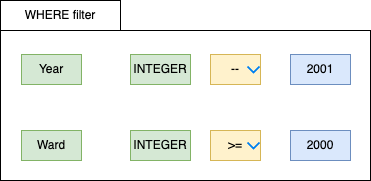
\includegraphics[width=0.4\linewidth]{../interface/WHERE_FILTER.png}
        \caption{Интерфейс отличий}
        \label{fig:where}

\end{figure}
    \subsection{Вывод отличий}
    % описать вывод отличий 
Сравнение сохраненного каталога с реальной схемой источника вызывается кнопкой и открывается отдельным модальным окном.
Отличия сгруппированы по типу: добавленные, измененные и удаленные колонки, каждая группа выводится своей таблицей.
Там же находится кнопка обновления каталога, неактивная, когда расхождений нет. Ниже на рисунке \ref{fig:showdiff} показан интерфейс. 

\begin{figure}[H] 
        \center
        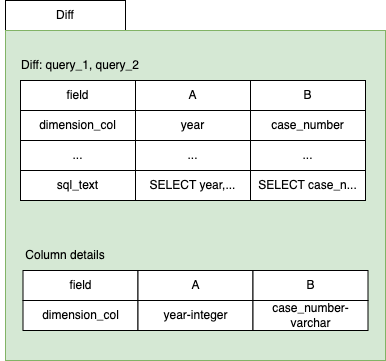
\includegraphics[width=0.4\linewidth]{../interface/DIFF.png}
        \caption{Интерфейс отличий}
        \label{fig:showdiff}
\end{figure}

    \subsection{Шаблон интерфейса}
    Ниже на рисунке \ref{fig:template_ui} продемонстрирован шаблон интерфейса собранный из форм и выводом графика.
    В последствие будет реализована рабочая версия интерфейса. 

    \begin{figure}[H]
        \center
        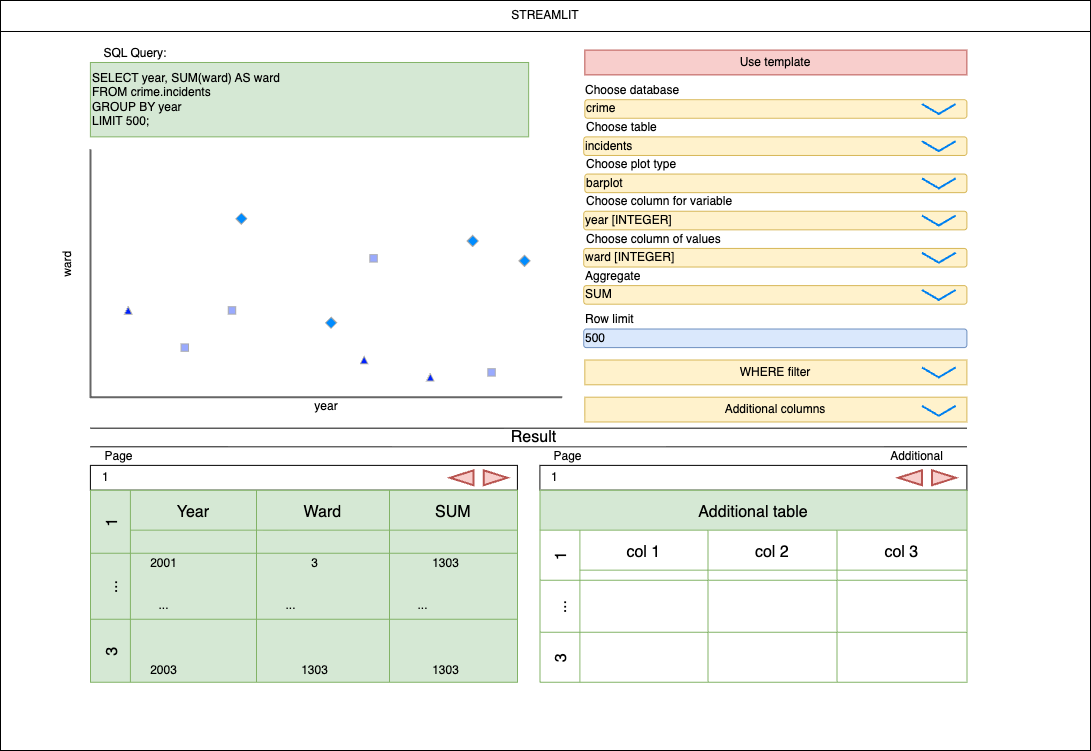
\includegraphics[width=0.6\linewidth]{../interface/TEMPLATE_UI.png}
        \caption{Шаблон интерфейса}
        \label{fig:template_ui}
    \end{figure}
    

\newpage
\section{Разработка интерфейса}

Интерфейс реализован на Streamlit и разделен на две части: 
справа находятся элементы управления и слева выводится SQL запрос и график, а 
снизу таблицы результата. Каждый элемент управления хранит свое значение в состоянии сессии (st.session\_state), 
и при любом изменении страница перерисовывается. 
Выбранные значения собираются в один словарь параметров (источник, таблица, вид графика, 
колонки, агрегатная функция, условия, лимит), который передается в функцию построения 
SQL запроса, после чего запрос отправляется RESTу источника.

\subsection{Поля ввода}
Текстовое поле используется там, где значение заранее неизвестно и его нельзя выбрать из списка. 
Основное поле это Row limit - ограничение на количество строк, 
которое подставляется в LIMIT запроса. Если поле пустое или введено не число,
 используется значение по умолчанию 500, 
поэтому неправильный ввод не ломает запрос. При смене таблицы или колонок поле сбрасывается, 
что бы лимит от прошлого запроса не переносился на новый.
Так же поля ввода есть в форме условий (значение для сравнения) и под таблицами результата (номер страницы). 
Поле создается методом st.text\_input, а номер страницы под таблицами - методом st.number\_input.
Ниже на рисунке \ref{fig:ui_input} показано само поле ввода.

\begin{figure}[H]
    \center
    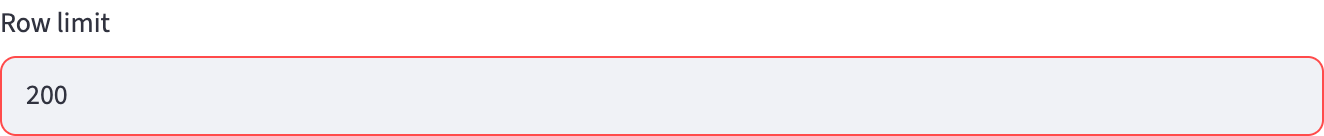
\includegraphics[width=0.6\linewidth]{img/UI_INPUT.png}
    \caption{Итоговый интерфейс поля ввода}
    \label{fig:ui_input}
\end{figure}

\subsection{Выпадающие списки}
Выпадающие списки используются для всех параметров, допустимые значения которых заранее известны из meta.catalog: выбор базы данных, таблицы, вида графика 
(barplot, pieplot, scatter, heatmap), колонки переменной, колонки значений и агрегатной функции (SUM, AVG, COUNT). 
Так пользователь не может выбрать несуществующую таблицу или колонку.
Рядом с именем колонки в квадратных скобках выводится короткое обозначение типа данных, 
которое берется из data\_type каталога, что бы было понятно какую колонку можно суммировать, считать среднее и т.д. 
После выбора базы список таблиц содержит только ее таблицы, а колонка значений не может совпадать с колонкой переменной.
Для heatmap появляется дополнительный список второй размерности, а для scatter список агрегатной функции скрывается, 
так как точки выводятся без группировки. 
Все выпадающие списки создаются методом st.selectbox.
Итоговый интерфейс выпадающего списка показан на рисунке \ref{fig:ui_dropdown}.

\begin{figure}[H]
    \center
    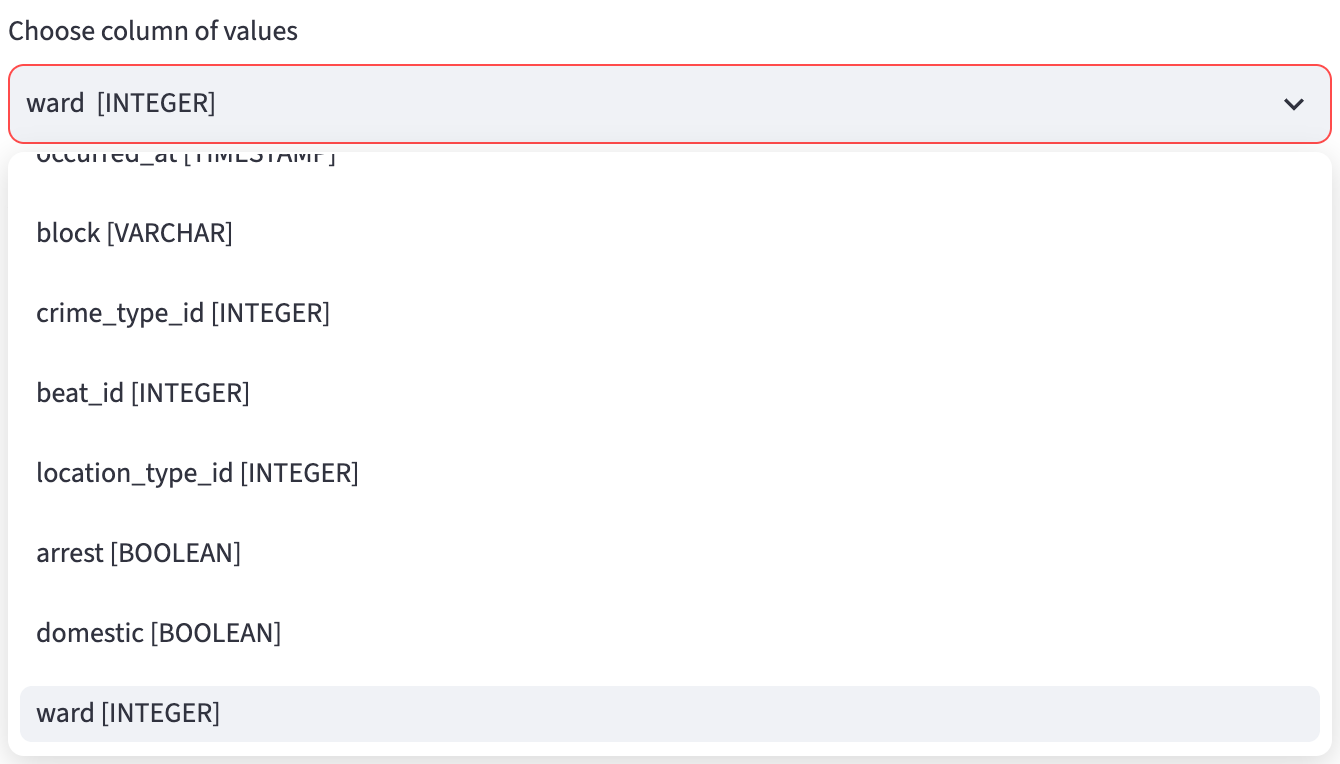
\includegraphics[width=0.6\linewidth]{img/UI_DROPDOWN.png}
    \caption{Итоговый интерфейс выпадающего списка}
    \label{fig:ui_dropdown}
\end{figure}

\subsection{Кнопки}
Кнопки отвечают за действия которые открывают отдельные окна (см. рис. \ref{fig:ui_buttons}):
\begin{itemize}
    \item Use template - открывает окно со списком сохраненных шаблонов из которого шаблон можно применить, удалить или сравнить с другим;
    \item Save query as template - сохраняет текущий запрос и параметры формы в базу шаблонов;
    \item Show diff - сравнивает сохраненный meta.catalog с реальной схемой источника.
\end{itemize}

Кнопки WHERE filter и Additional columns открывают всплывающие панели, они описаны ниже.
Кнопки создаются методом st.button, а открываемые ими окна - декоратором @st.dialog.

\begin{figure}[H]
    \center
    
\includegraphics[width=0.6\linewidth]{img/UI_BUTTONS.png}
    \caption{Итоговый интерфейс кнопок}
    \label{fig:ui_buttons}
\end{figure}

\subsection{Выбор нескольких атрибутов}
Панель Additional columns содержит все остальные колонки выбранной таблицы (кроме колонки переменной и колонки значений), каждая с флажком и типом. 
Она нужна что бы кроме агрегированного результата посмотреть исходные строки. 
По отмеченным колонкам строится отдельный запрос без группировки 
с теми же условиями и лимитом, и его результат выводится второй таблицей Details рядом с основной. 
Панель создается методом st.popover, флажки - методом st.checkbox, а таблица Details выводится методом st.dataframe.
Ниже на рисунке \ref{fig:ui_additional} показан выбор нескольких атрибутов.

\begin{figure}[H]
    \center
    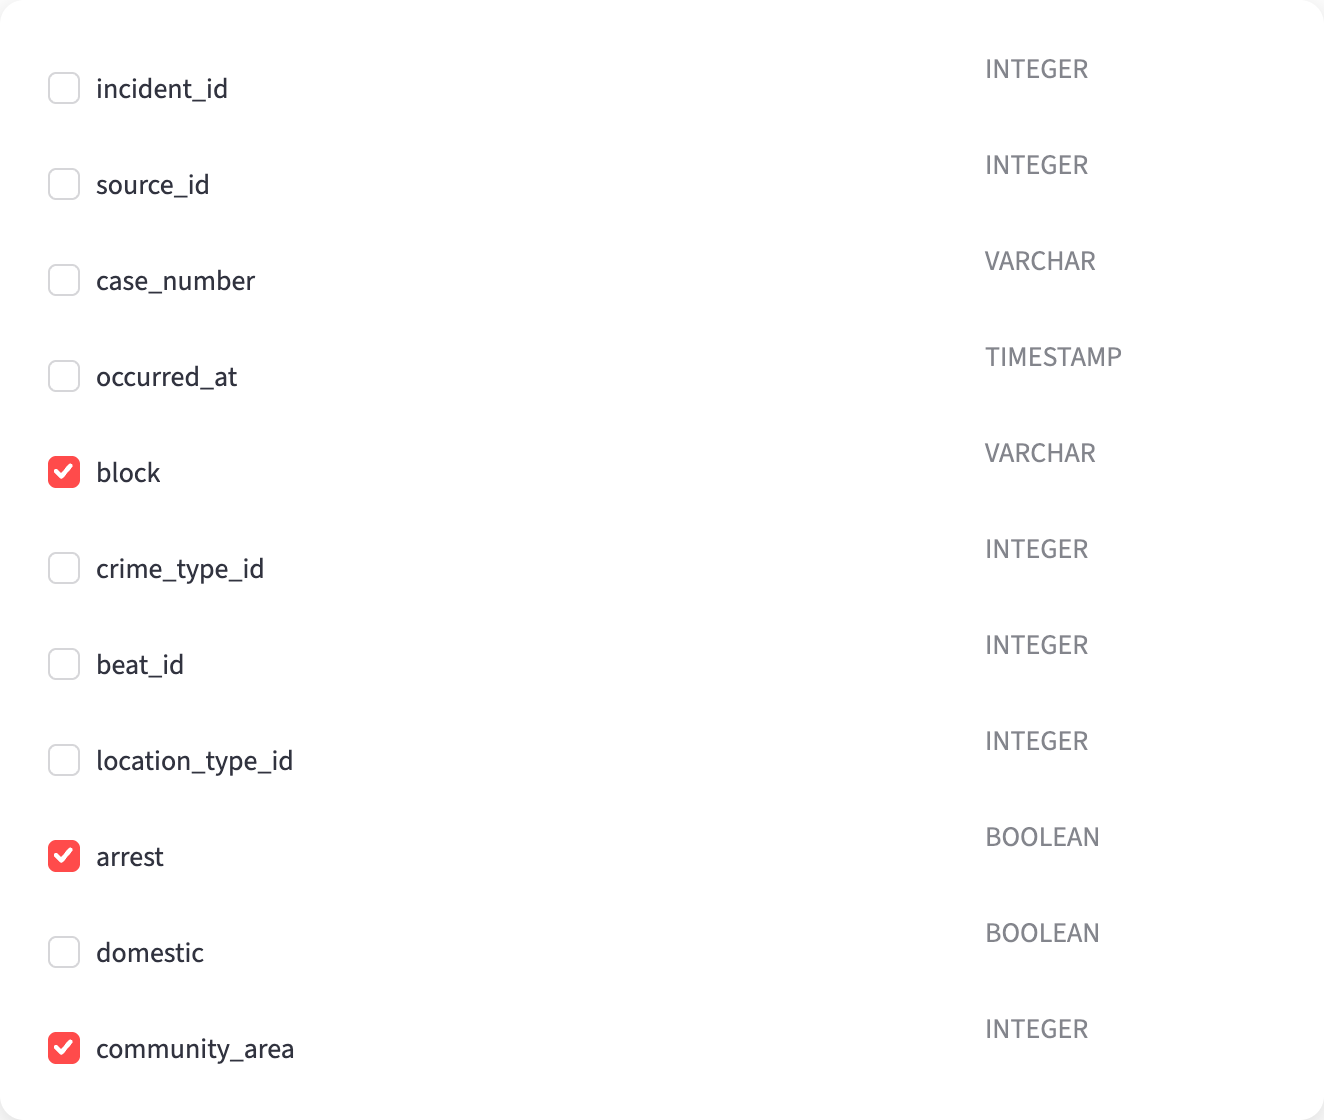
\includegraphics[width=0.5\linewidth]{img/UI_ADDITIONAL.png}
    \caption{Итоговый интерфейс выбора нескольких атрибутов}
    \label{fig:ui_additional}
\end{figure}

\subsection{Форма выбора шаблона}
Форма открывается кнопкой Use template в окне и выводит все шаблоны из базы шаблонов. Каждая строка содержит кнопку с описанием шаблона 
(имя, источник и таблица, вид графика и колонки), флажок compare и кнопку Delete. 
При нажатии на шаблон его параметры записываются в состояние сессии, то есть все выпадающие списки и поле лимита заполняются значениями из шаблона, 
и запрос строится заново, а в базе шаблонов увеличивается счетчик использования. Окно создается декоратором @st.dialog, шаблоны и кнопка Delete - методом st.button, флажок compare - методом st.checkbox.
Итоговый интерфейс формы показан на рисунке \ref{fig:ui_templates}.

\begin{figure}[H]
    \center
    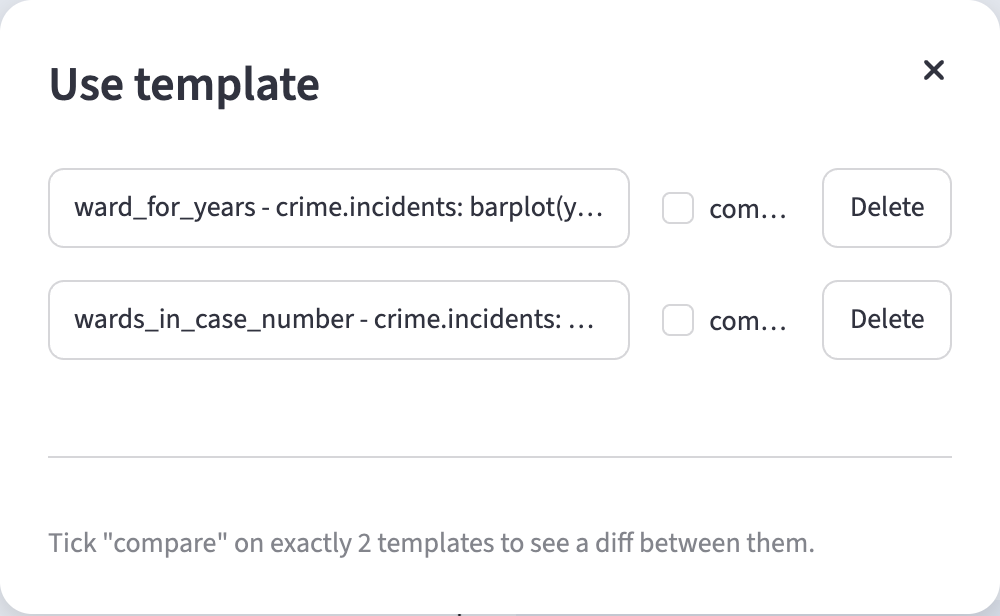
\includegraphics[width=0.5\linewidth]{img/UI_TEMPLATES.png}
    \caption{Итоговый интерфейс формы выбора шаблона}
    \label{fig:ui_templates}
\end{figure}

\subsection{Форма для условий}
Форма WHERE filter открывается всплывающей панелью и содержит строку для колонки переменной и колонки значений. 
В строке выводится имя колонки, ее тип, выпадающий список оператора и поле для значения. 
Для числовых колонок доступны операторы $=, <, >, \leq, \geq$, значение - означает, что условие не задано. 
Для строковых колонок введенный текст ищется через LIKE.
Условие добавляется в запрос только если выбран оператор и введено значение, несколько условий объединяются через AND. 
На рисунке \ref{fig:ui_where} задано условие year $\geq$ 2010, которое в запросе превращается в WHERE year >= 2010 (см. рис. \ref{fig:ui_final}).
Панель создается методом st.popover, оператор выбирается через st.selectbox, значение вводится через st.text\_input.

\begin{figure}[H]
    \center
    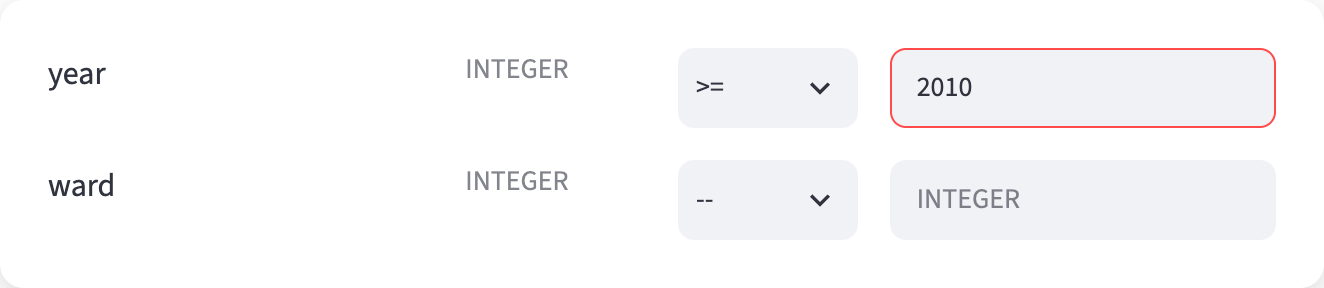
\includegraphics[width=0.6\linewidth]{img/UI_WHERE.png}
    \caption{Итоговый интерфейс формы условий}
    \label{fig:ui_where}
\end{figure}

\subsection{Форма для сравнений}
В интерфейсе есть два вида сравнения. 
Первое - сравнение двух шаблонов: в форме выбора шаблона нужно отметить флажок compare у двух шаблонов, 
и ниже появится таблица отличающихся полей (колонки, условия, лимит, текст запроса) и таблица Column details, 
где для колонок шаблонов из meta.catalog подставлен их тип (см. рис. \ref{fig:ui_compare}).
Таблицы отличий выводятся методом st.dataframe.

\begin{figure}[H]
    \center
    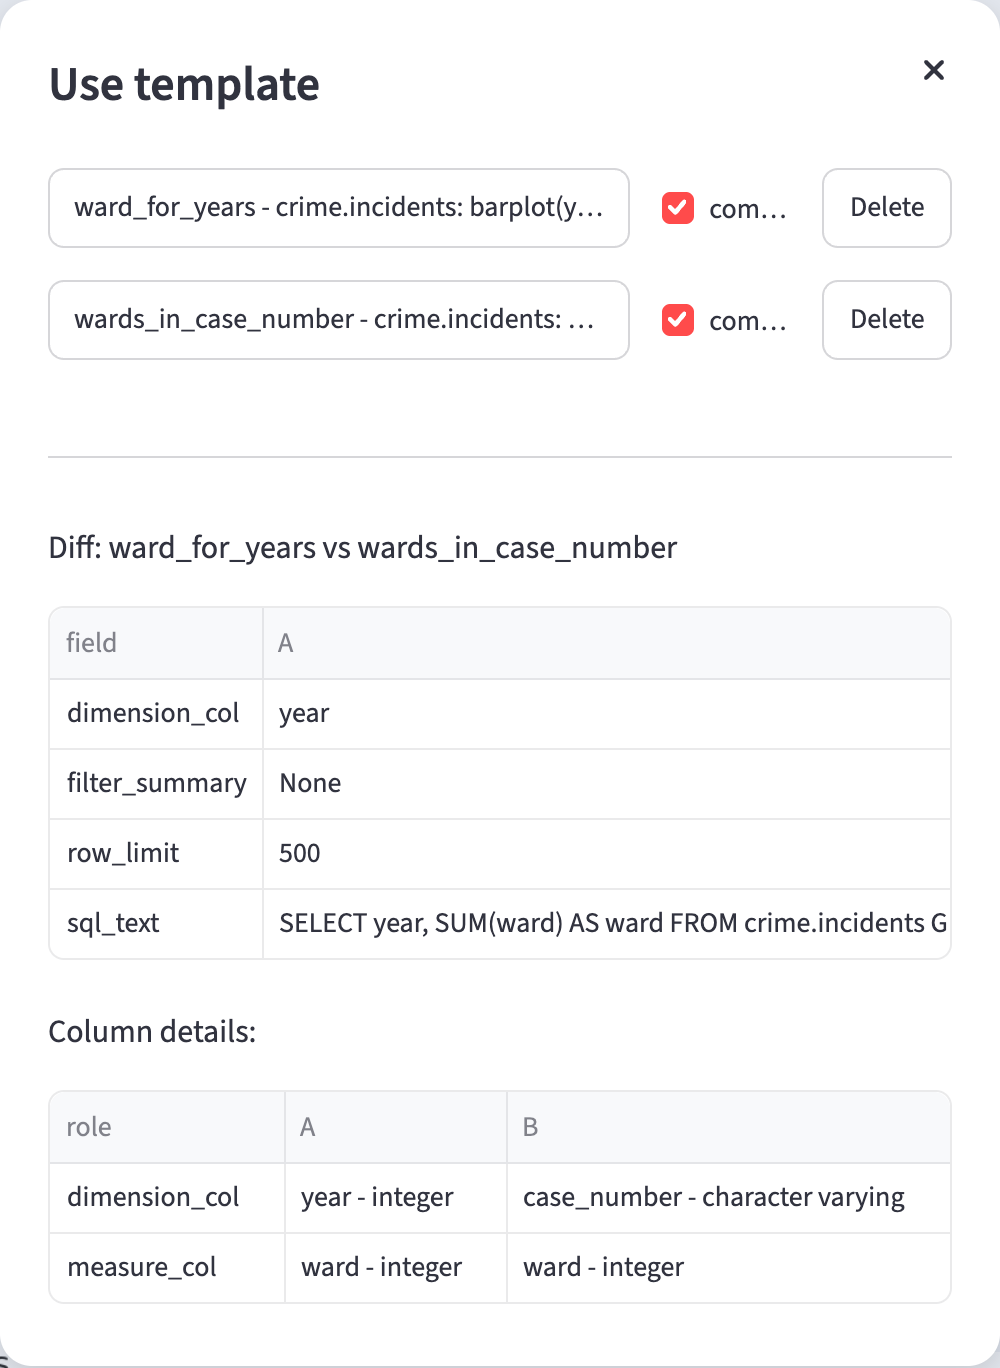
\includegraphics[width=0.5\linewidth]{img/UI_COMPARE.png}
    \caption{Итоговый интерфейс сравнения шаблонов}
    \label{fig:ui_compare}
\end{figure}

Второе - сравнение каталога с источником (Show diff). 
Окно показывает количество добавленных, измененных и удаленных колонок и таблицу для каждой группы. 
Кнопка Update синхронизирует meta.catalog с источником и неактивна, если отличий нет, как на рисунке \ref{fig:ui_showdiff}.
Окно создается декоратором @st.dialog, количество отличий выводится через st.write, а таблицы групп - через st.dataframe.

\begin{figure}[H]
    \center
    
\includegraphics[width=0.5\linewidth]{img/UI_SHOWDIFF.png}
    \caption{Итоговый интерфейс сравнения каталога с источником}
    \label{fig:ui_showdiff}
\end{figure}

\subsection{Результат}
На рисунке \ref{fig:ui_final} показан итоговый интерфейс, собранный из всех описанных элементов. Выбрана база crime, таблица incidents, 
столбчатый график суммы ward по year с условием year $\geq$ 2010 и лимитом 200. 
Слева сверху выводится итоговый SQL запрос, под ним график, снизу таблица Result с результатом запроса и таблица Details с дополнительными колонками. 
Обе таблицы выводятся постранично по 10 строк, под каждой указан диапазон строк и общее их количество.
Страница делится на колонки методом st.columns, SQL запрос выводится через st.code, график - через st.pyplot, таблицы - через st.dataframe, подписи под ними - через st.caption.

\begin{figure}[H]
    \center
    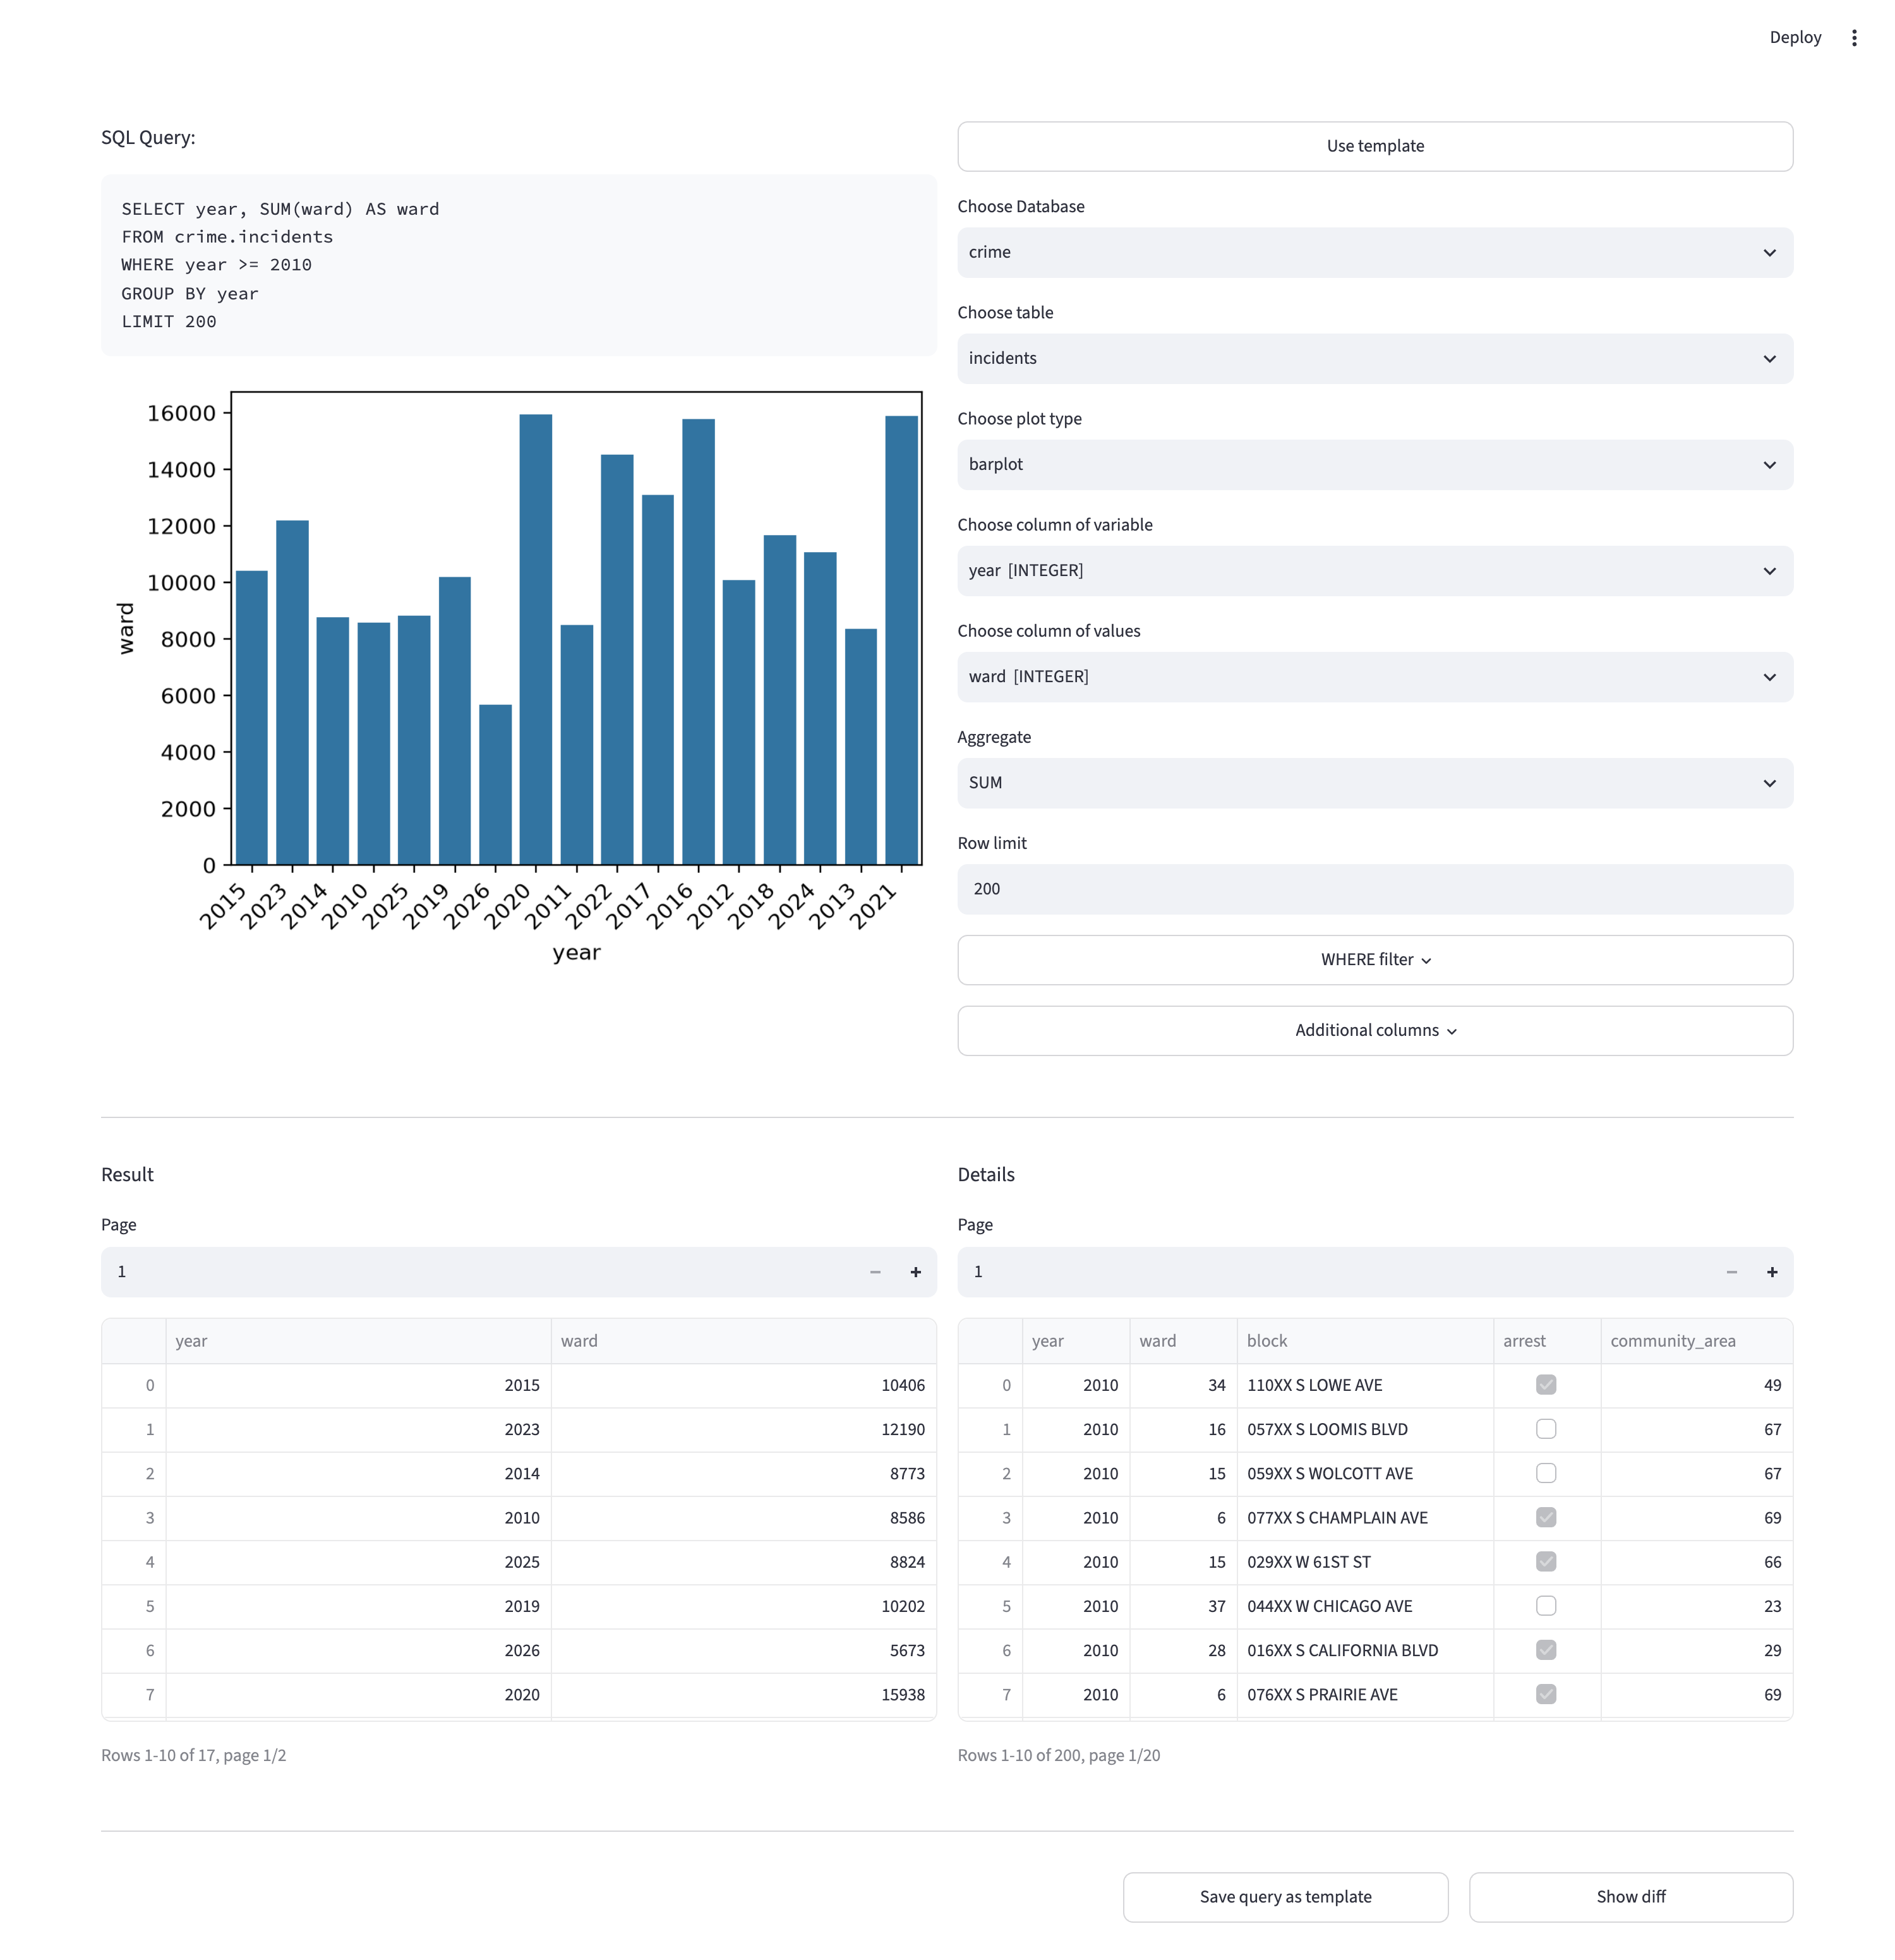
\includegraphics[width=\linewidth]{img/UI_FINAL.png}
    \caption{Итоговый интерфейс}
    \label{fig:ui_final}
\end{figure}


\newpage
\section{Результаты работы}

\subsection{Сценарий 1}
Вывод первых 500 результатов горнолыжников из таблицы result базы mountain\_sport, где attempt1\_result $>$ 0, в виде диаграммы рассеивания времени первой попытки (attempt1\_result) против второй (attempt2\_result).
Итоговый SQL запрос приведен в листинге \ref{lis:scen1}, результат на рисунке \ref{fig:scen1}.
\begin{lstlisting}[language=SQL, caption={Сценарий 1: итоговый SQL запрос}, label={lis:scen1}]
SELECT attempt1_result, attempt2_result
FROM mountain_sport.result
WHERE attempt1_result > 0
LIMIT 500
\end{lstlisting}
\begin{figure}[H]
    \center
    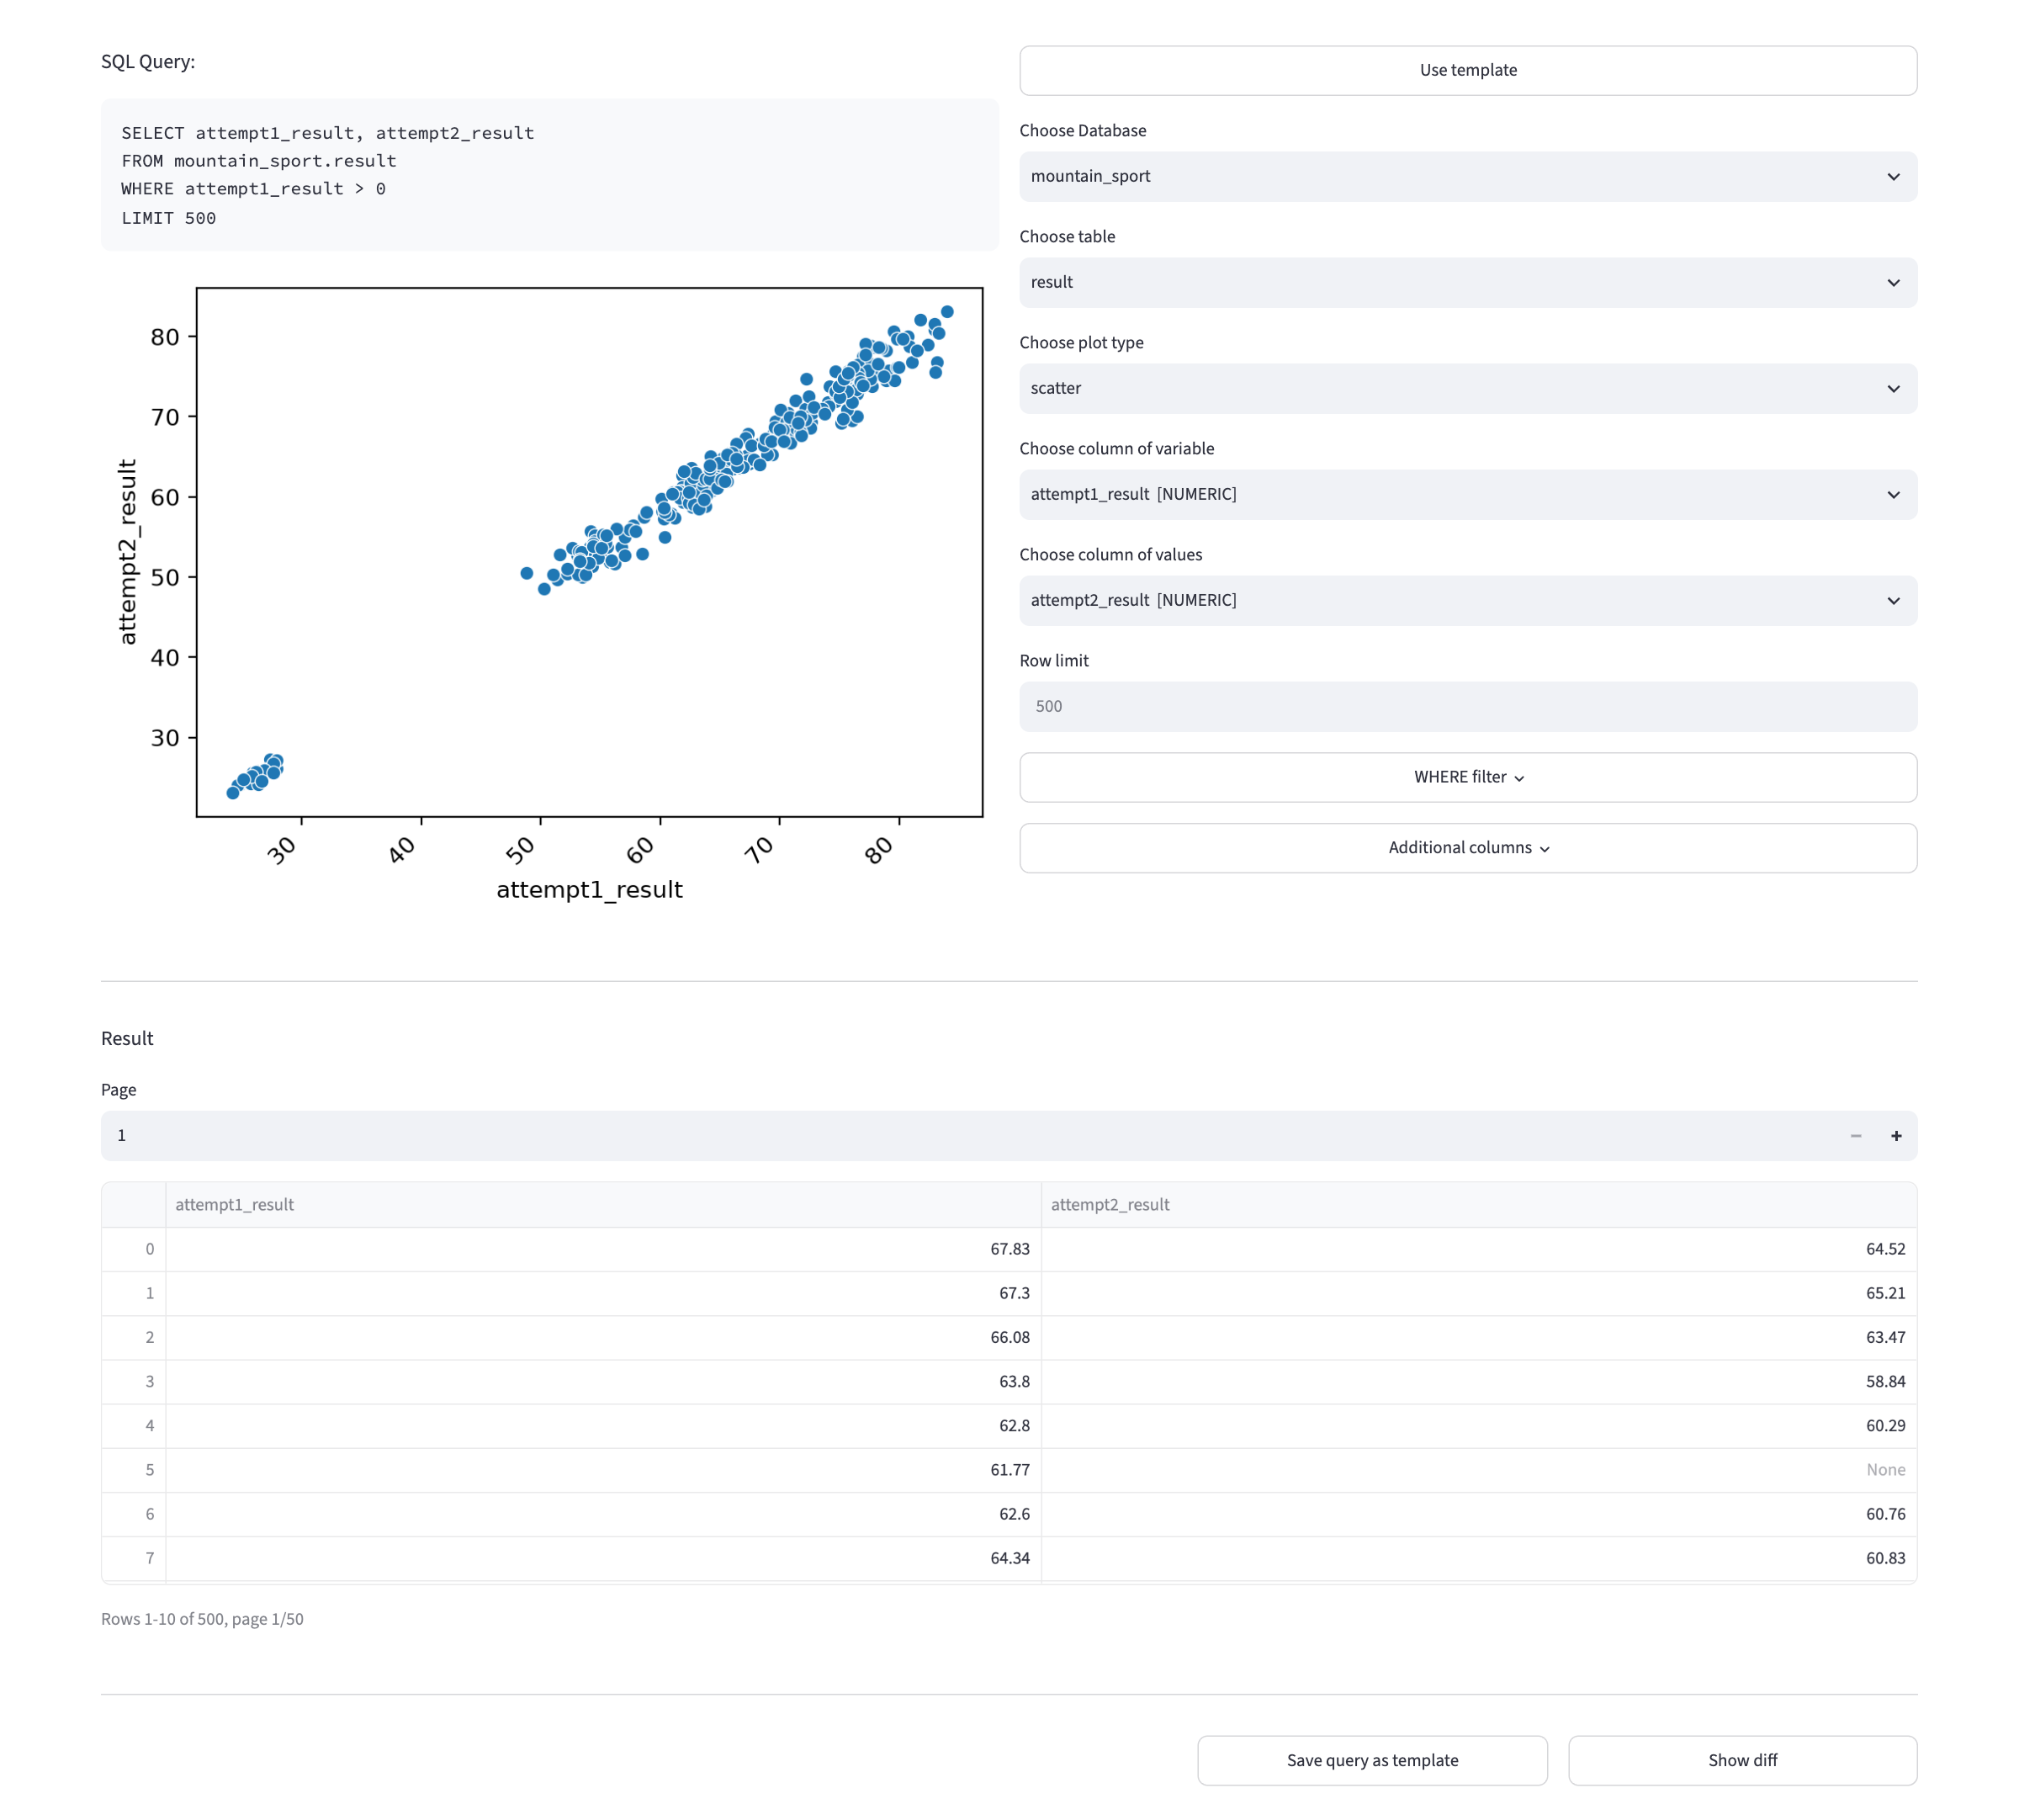
\includegraphics[width=\linewidth]{img/SCEN_1.png}
    \caption{Сценарий 1}
    \label{fig:scen1}
\end{figure}

\subsection{Сценарий 2}
Вывод столбчатой диаграммы суммарной стоимости занятий SUM(cost) по предметам subject\_id из таблицы lesson базы extra\_for\_students, где стоимость cost $\geq$ 1000 рублей.
Итоговый SQL запрос приведен в листинге \ref{lis:scen2}, результат на рисунке \ref{fig:scen2}.
\begin{lstlisting}[language=SQL, caption={Сценарий 2: итоговый SQL запрос}, label={lis:scen2}]
SELECT subject_id, SUM(cost) AS cost
FROM extra_for_students.lesson
WHERE cost >= 1000
GROUP BY subject_id
LIMIT 500
\end{lstlisting}
\begin{figure}[H]
    \center
    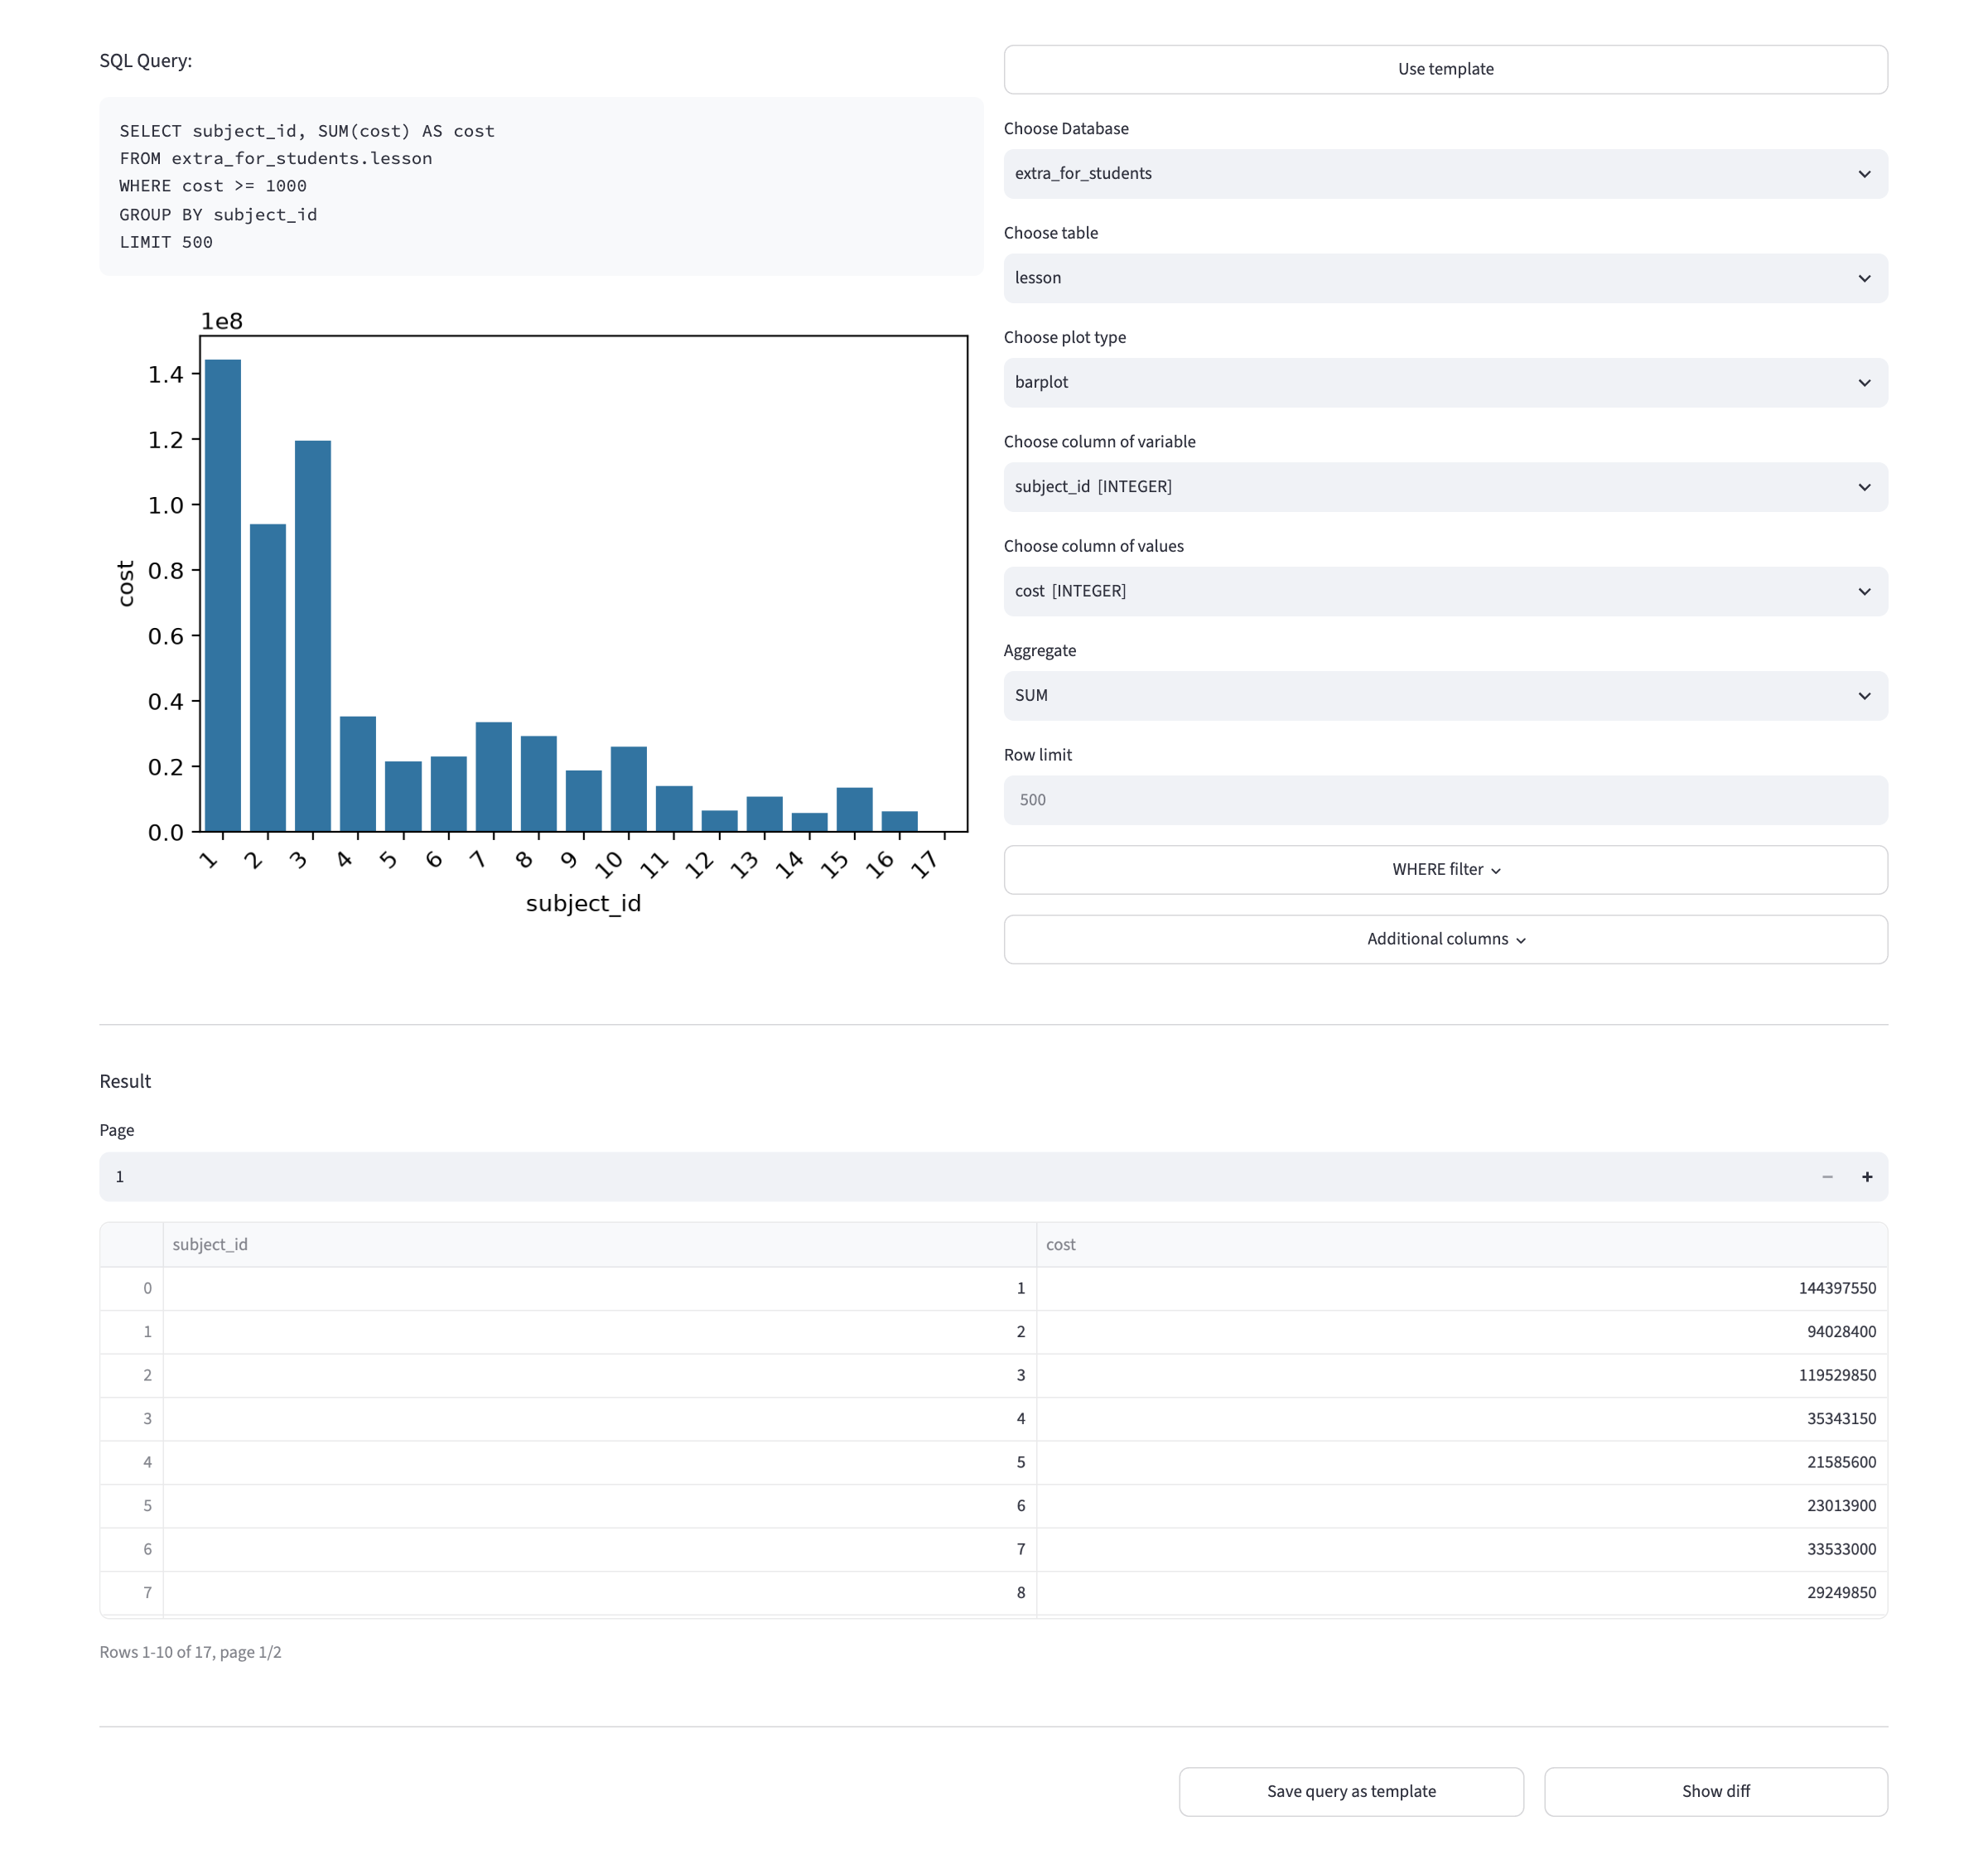
\includegraphics[width=\linewidth]{img/SCEN_2.png}
    \caption{Сценарий 2}
    \label{fig:scen2}
\end{figure}

\subsection{Сценарий 3}
Вывод круговой диаграммы доли выступлений по номинациям COUNT(perfomance\_id) по perfomance\_type из таблицы perfomance базы sport\_and\_cheerleaders.
Итоговый SQL запрос приведен в листинге \ref{lis:scen3}, результат на рисунке \ref{fig:scen3}.
\begin{lstlisting}[language=SQL, caption={Сценарий 3: итоговый SQL запрос}, label={lis:scen3}]
SELECT perfomance_type, COUNT(perfomance_id) AS perfomance_id
FROM sport_and_cheerleaders.perfomance
GROUP BY perfomance_type
LIMIT 500
\end{lstlisting}
\begin{figure}[H]
    \center
    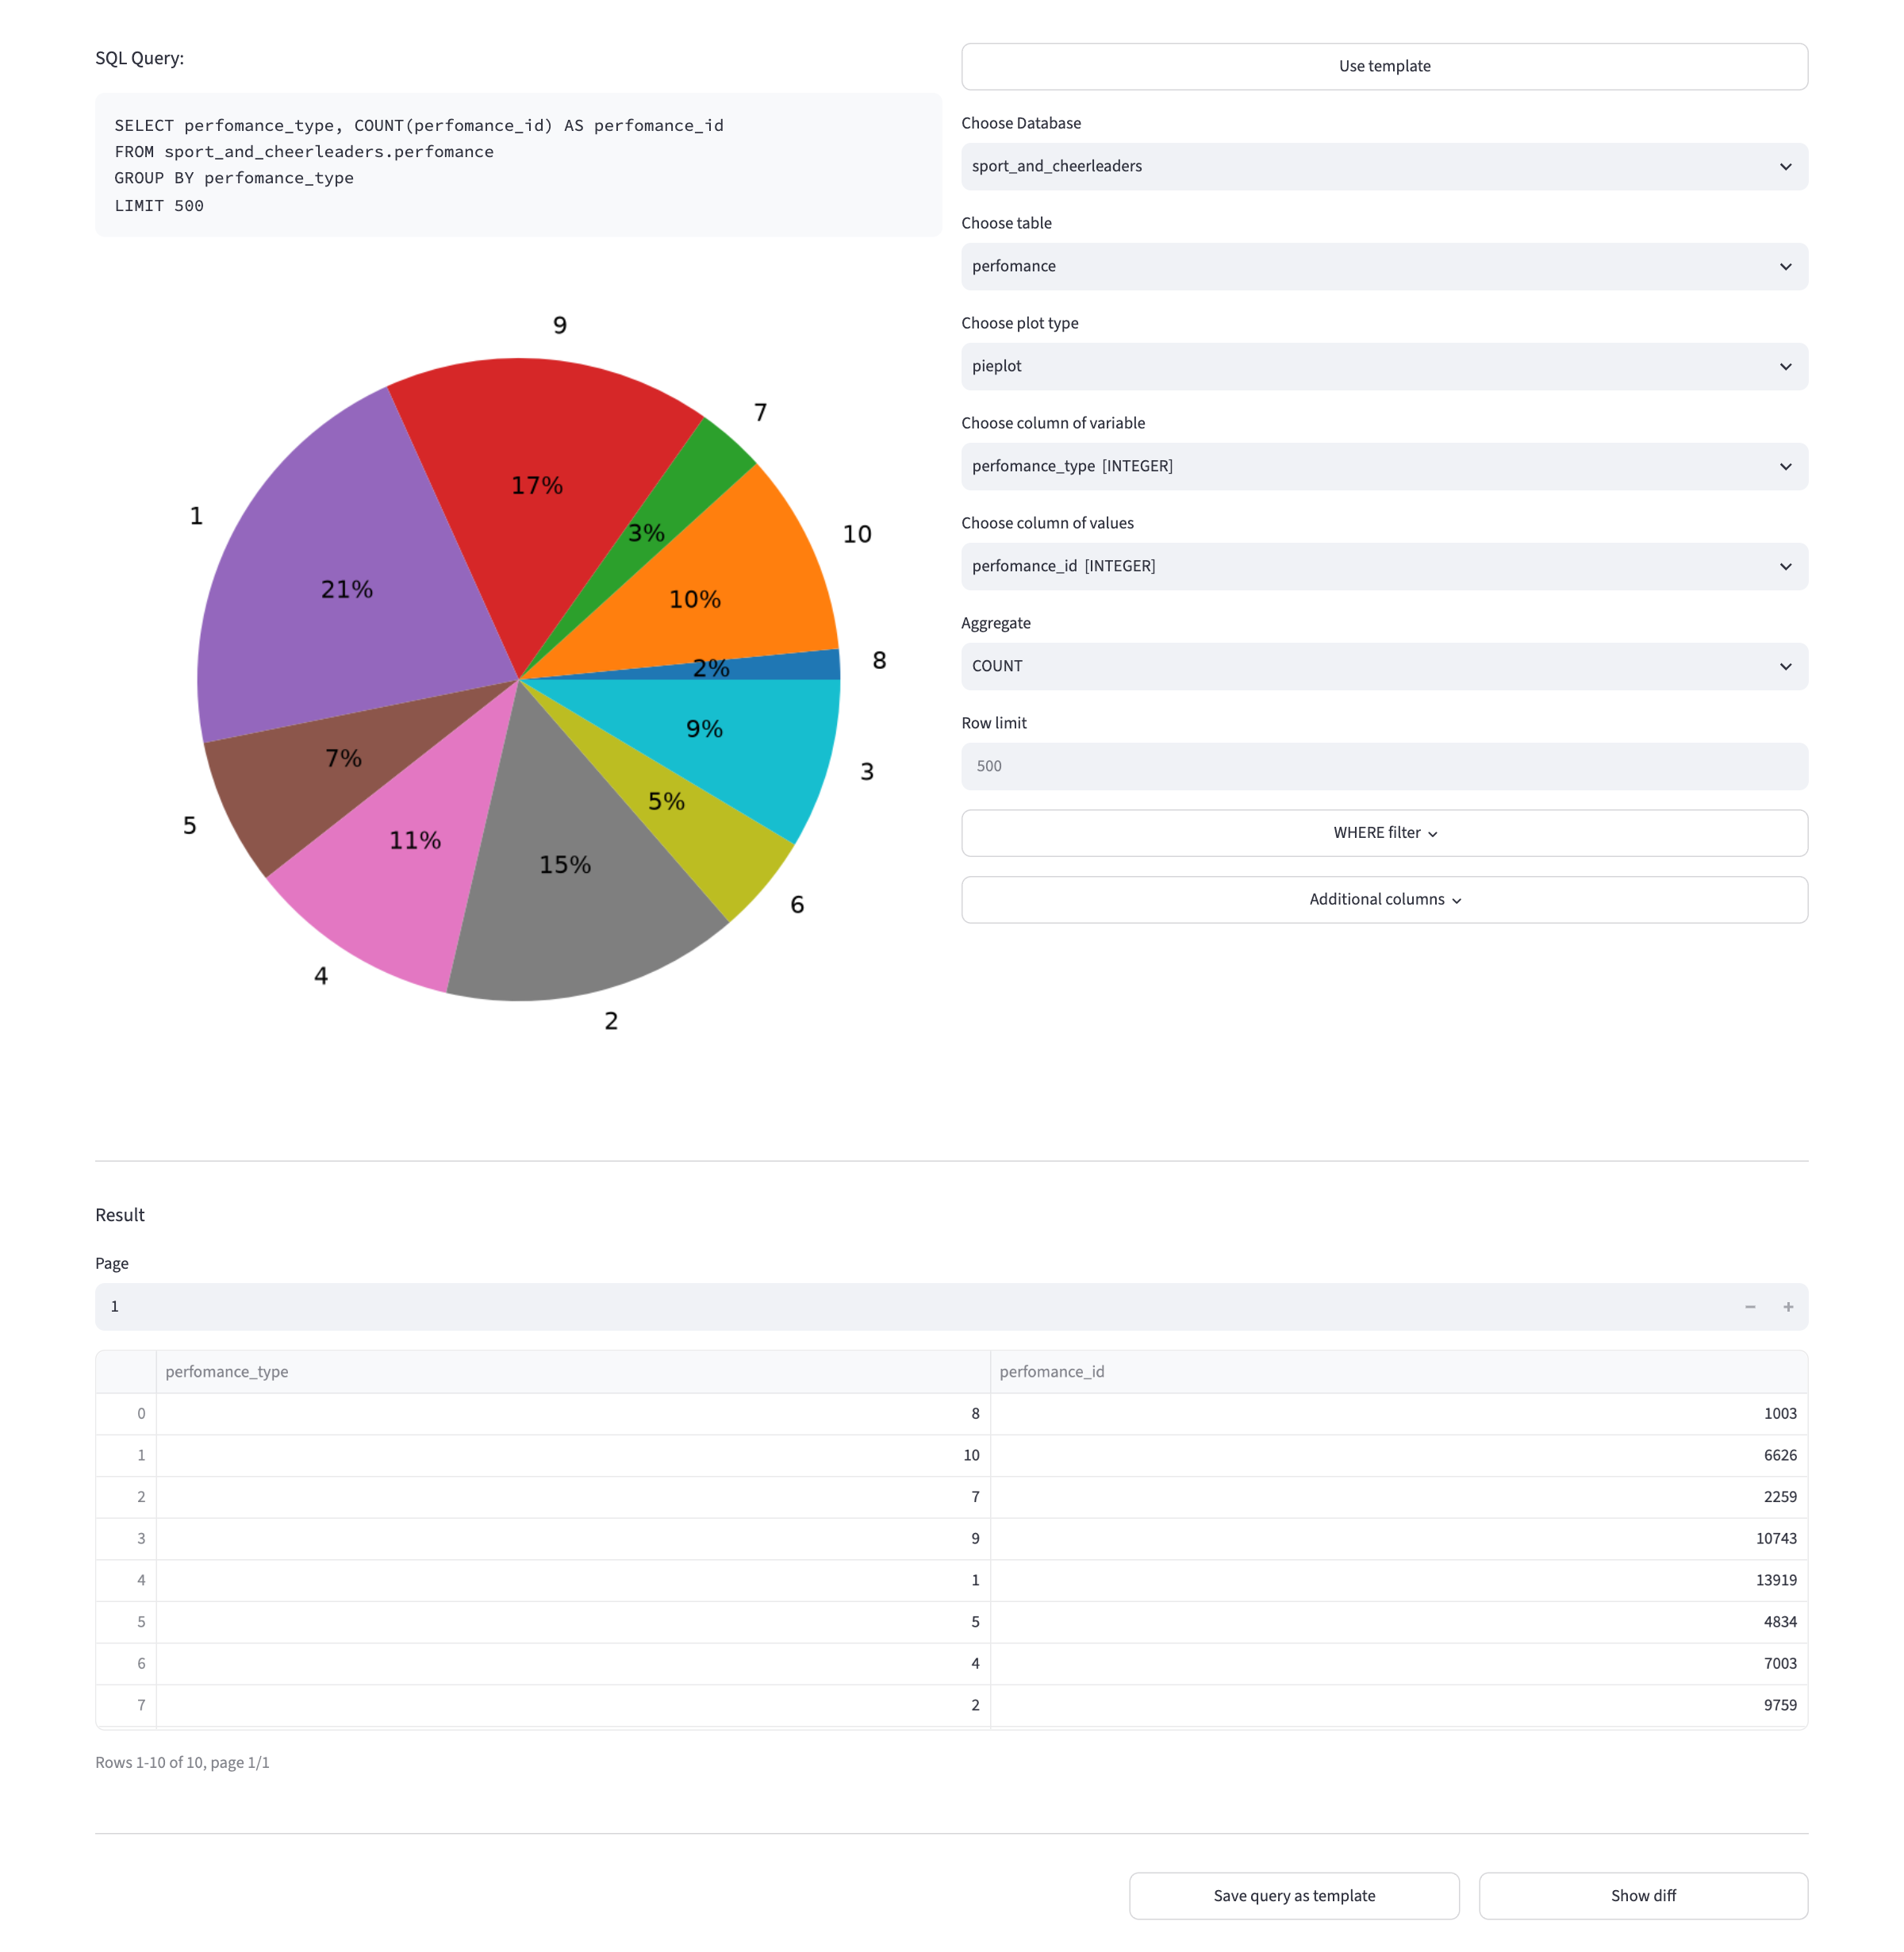
\includegraphics[width=\linewidth]{img/SCEN_3.png}
    \caption{Сценарий 3}
    \label{fig:scen3}
\end{figure}

\subsection{Сценарий 4}
Вывод тепловой карты средней стоимости занятия AVG(cost) по предметам subject\_id и форматам format\_id из таблицы lesson базы extra\_for\_students.
Итоговый SQL запрос приведен в листинге \ref{lis:scen4}, результат на рисунке \ref{fig:scen4}.
\begin{lstlisting}[language=SQL, caption={Сценарий 4: итоговый SQL запрос}, label={lis:scen4}]
SELECT subject_id, format_id, AVG(cost) AS cost
FROM extra_for_students.lesson
GROUP BY subject_id, format_id
LIMIT 500
\end{lstlisting}
\begin{figure}[H]
    \center
    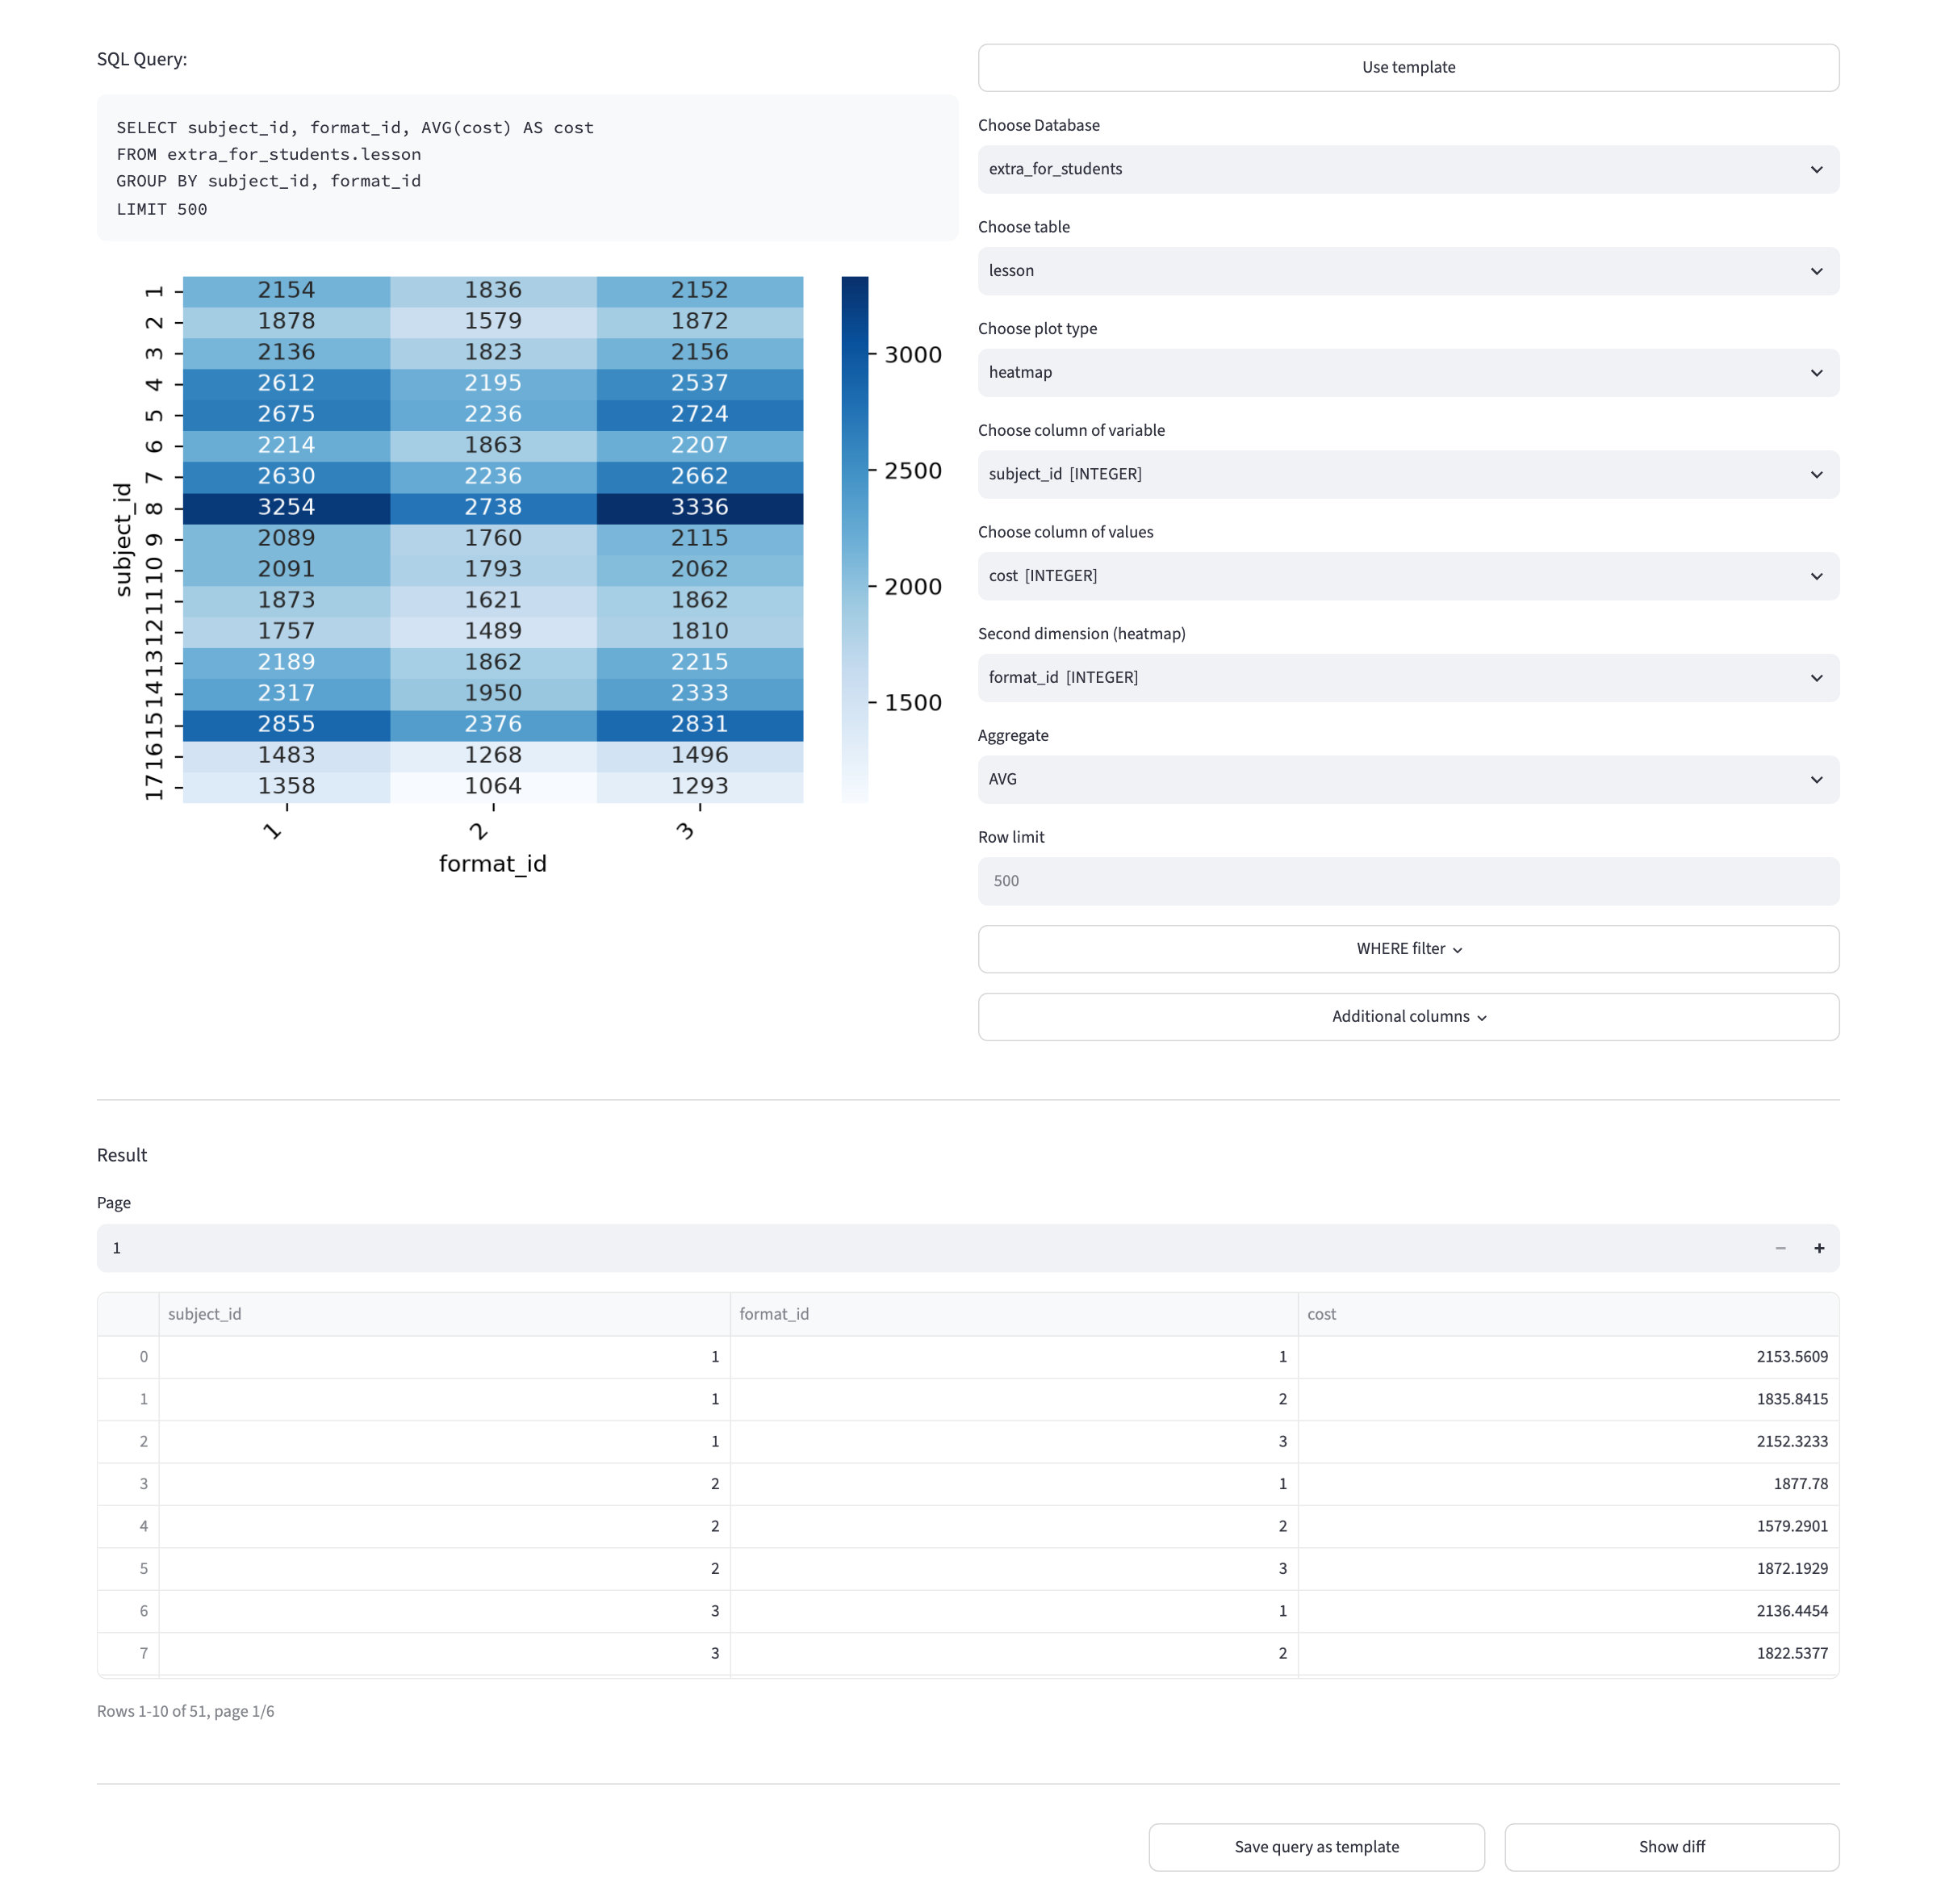
\includegraphics[width=\linewidth]{img/SCEN_4.png}
    \caption{Сценарий 4}
    \label{fig:scen4}
\end{figure}

\subsection{Сценарий 5}
Сравнение двух сохраненных шаблонов по таблице lesson - SUM(cost) по subject\_id без условия и с условием cost $\geq$ 1000 и лимитом 10 - через флажки compare в форме выбора шаблона.
Итоговые SQL запросы сравниваемых шаблонов приведены в листингах \ref{lis:scen5a} и \ref{lis:scen5b}, результат сравнения на рисунке \ref{fig:scen5}.
\begin{lstlisting}[language=SQL, caption={Сценарий 5: шаблон lesson\_cost\_by\_subject}, label={lis:scen5a}]
SELECT subject_id, SUM(cost) AS cost
FROM extra_for_students.lesson
GROUP BY subject_id
LIMIT 500
\end{lstlisting}
\begin{lstlisting}[language=SQL, caption={Сценарий 5: шаблон lesson\_cost\_by\_subject\_1000}, label={lis:scen5b}]
SELECT subject_id, SUM(cost) AS cost
FROM extra_for_students.lesson
WHERE cost >= 1000
GROUP BY subject_id
LIMIT 10
\end{lstlisting}
\begin{figure}[H]
    \center
    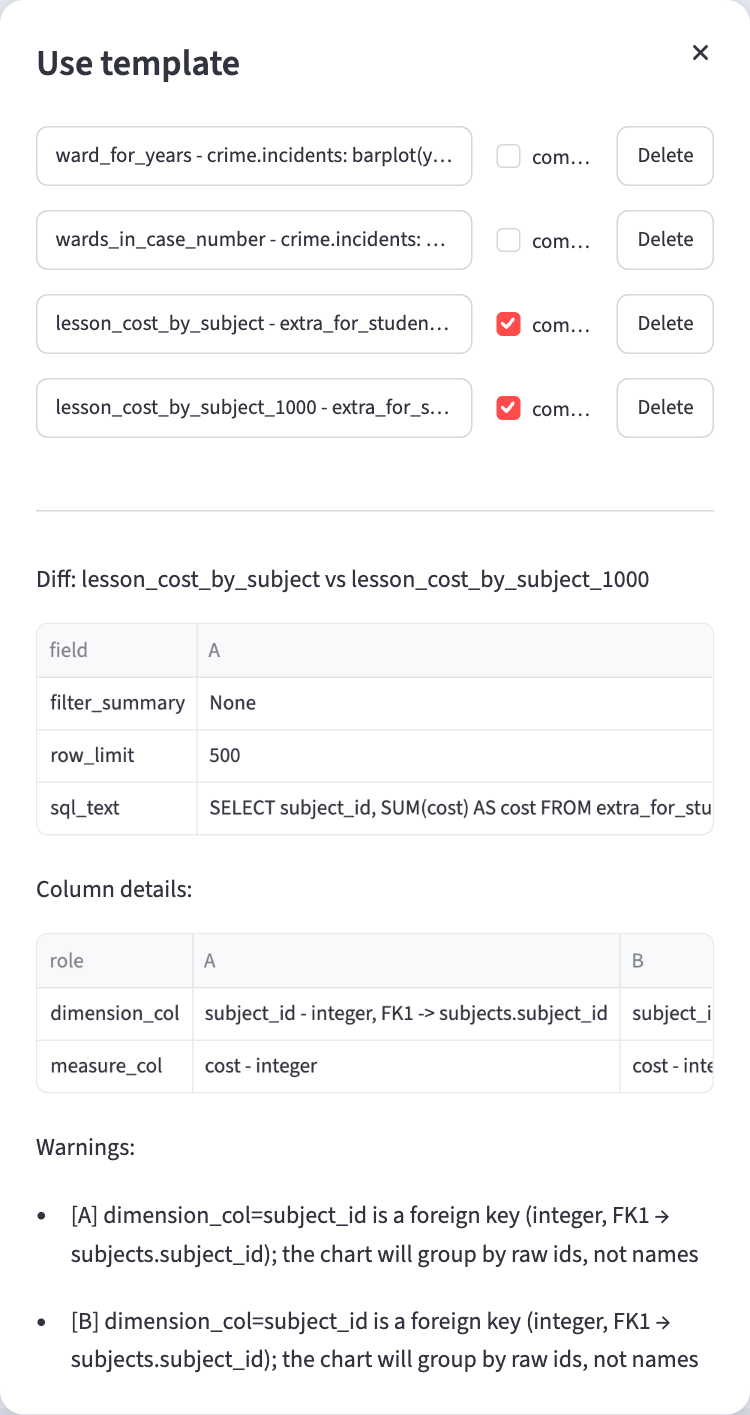
\includegraphics[width=0.5\linewidth]{img/SCEN_5.png}
    \caption{Сценарий 5: сравнение двух шаблонов}
    \label{fig:scen5}
\end{figure}

\subsection{Сценарий 6}
Добавление в источнике mountain\_sport новой колонки в таблицу athlete, ее обнаружение кнопкой Show diff как добавленной и синхронизация meta.catalog кнопкой Update.
Изменение источника приведено в листинге \ref{lis:scen6}, найденное отличие и состояние после обновления на рисунках \ref{fig:scen6} и \ref{fig:scen6u}.
\begin{lstlisting}[language=SQL, caption={Сценарий 6: изменение схемы источника}, label={lis:scen6}]
ALTER TABLE mountain_sport.athlete ADD COLUMN height SMALLINT;
\end{lstlisting}
\begin{figure}[H]
    \center
    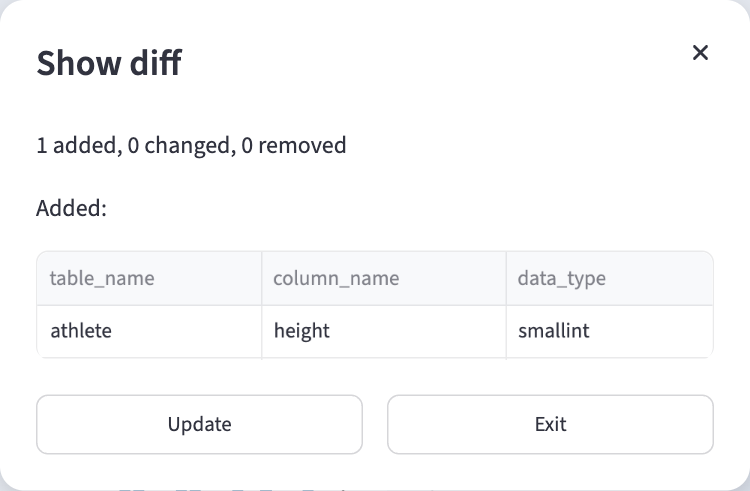
\includegraphics[width=0.5\linewidth]{img/SCEN_6.png}
    \caption{Сценарий 6: найденное отличие источника}
    \label{fig:scen6}
\end{figure}
\begin{figure}[H]
    \center
    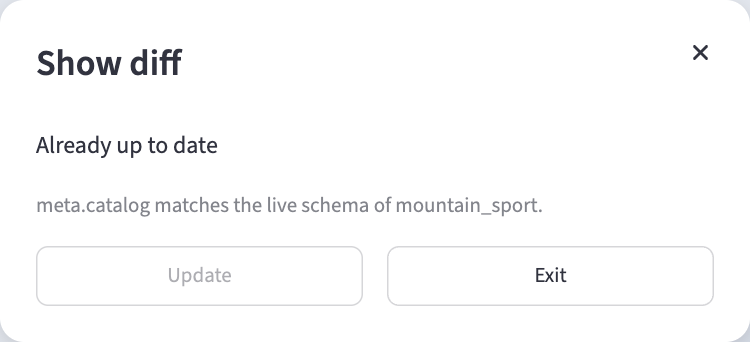
\includegraphics[width=0.5\linewidth]{img/SCEN_6_UPDATED.png}
    \caption{Сценарий 6: каталог после обновления}
    \label{fig:scen6u}
\end{figure}

\subsection{Сценарий 7}
Вывод количества спортсменов COUNT(sportsman\_id) по клубам club\_id из таблицы sportsman базы sport\_and\_cheerleaders, где club\_id $\leq$ 50, с дополнительными колонками sportsman\_lastname и sportsman\_birthdate в таблице Details.
Итоговый SQL запрос приведен в листинге \ref{lis:scen7}, результат на рисунке \ref{fig:scen7}.
\begin{lstlisting}[language=SQL, caption={Сценарий 7: итоговый SQL запрос}, label={lis:scen7}]
SELECT club_id, COUNT(sportsman_id) AS sportsman_id
FROM sport_and_cheerleaders.sportsman
WHERE club_id <= 50
GROUP BY club_id
LIMIT 500
\end{lstlisting}
\begin{figure}[H]
    \center
    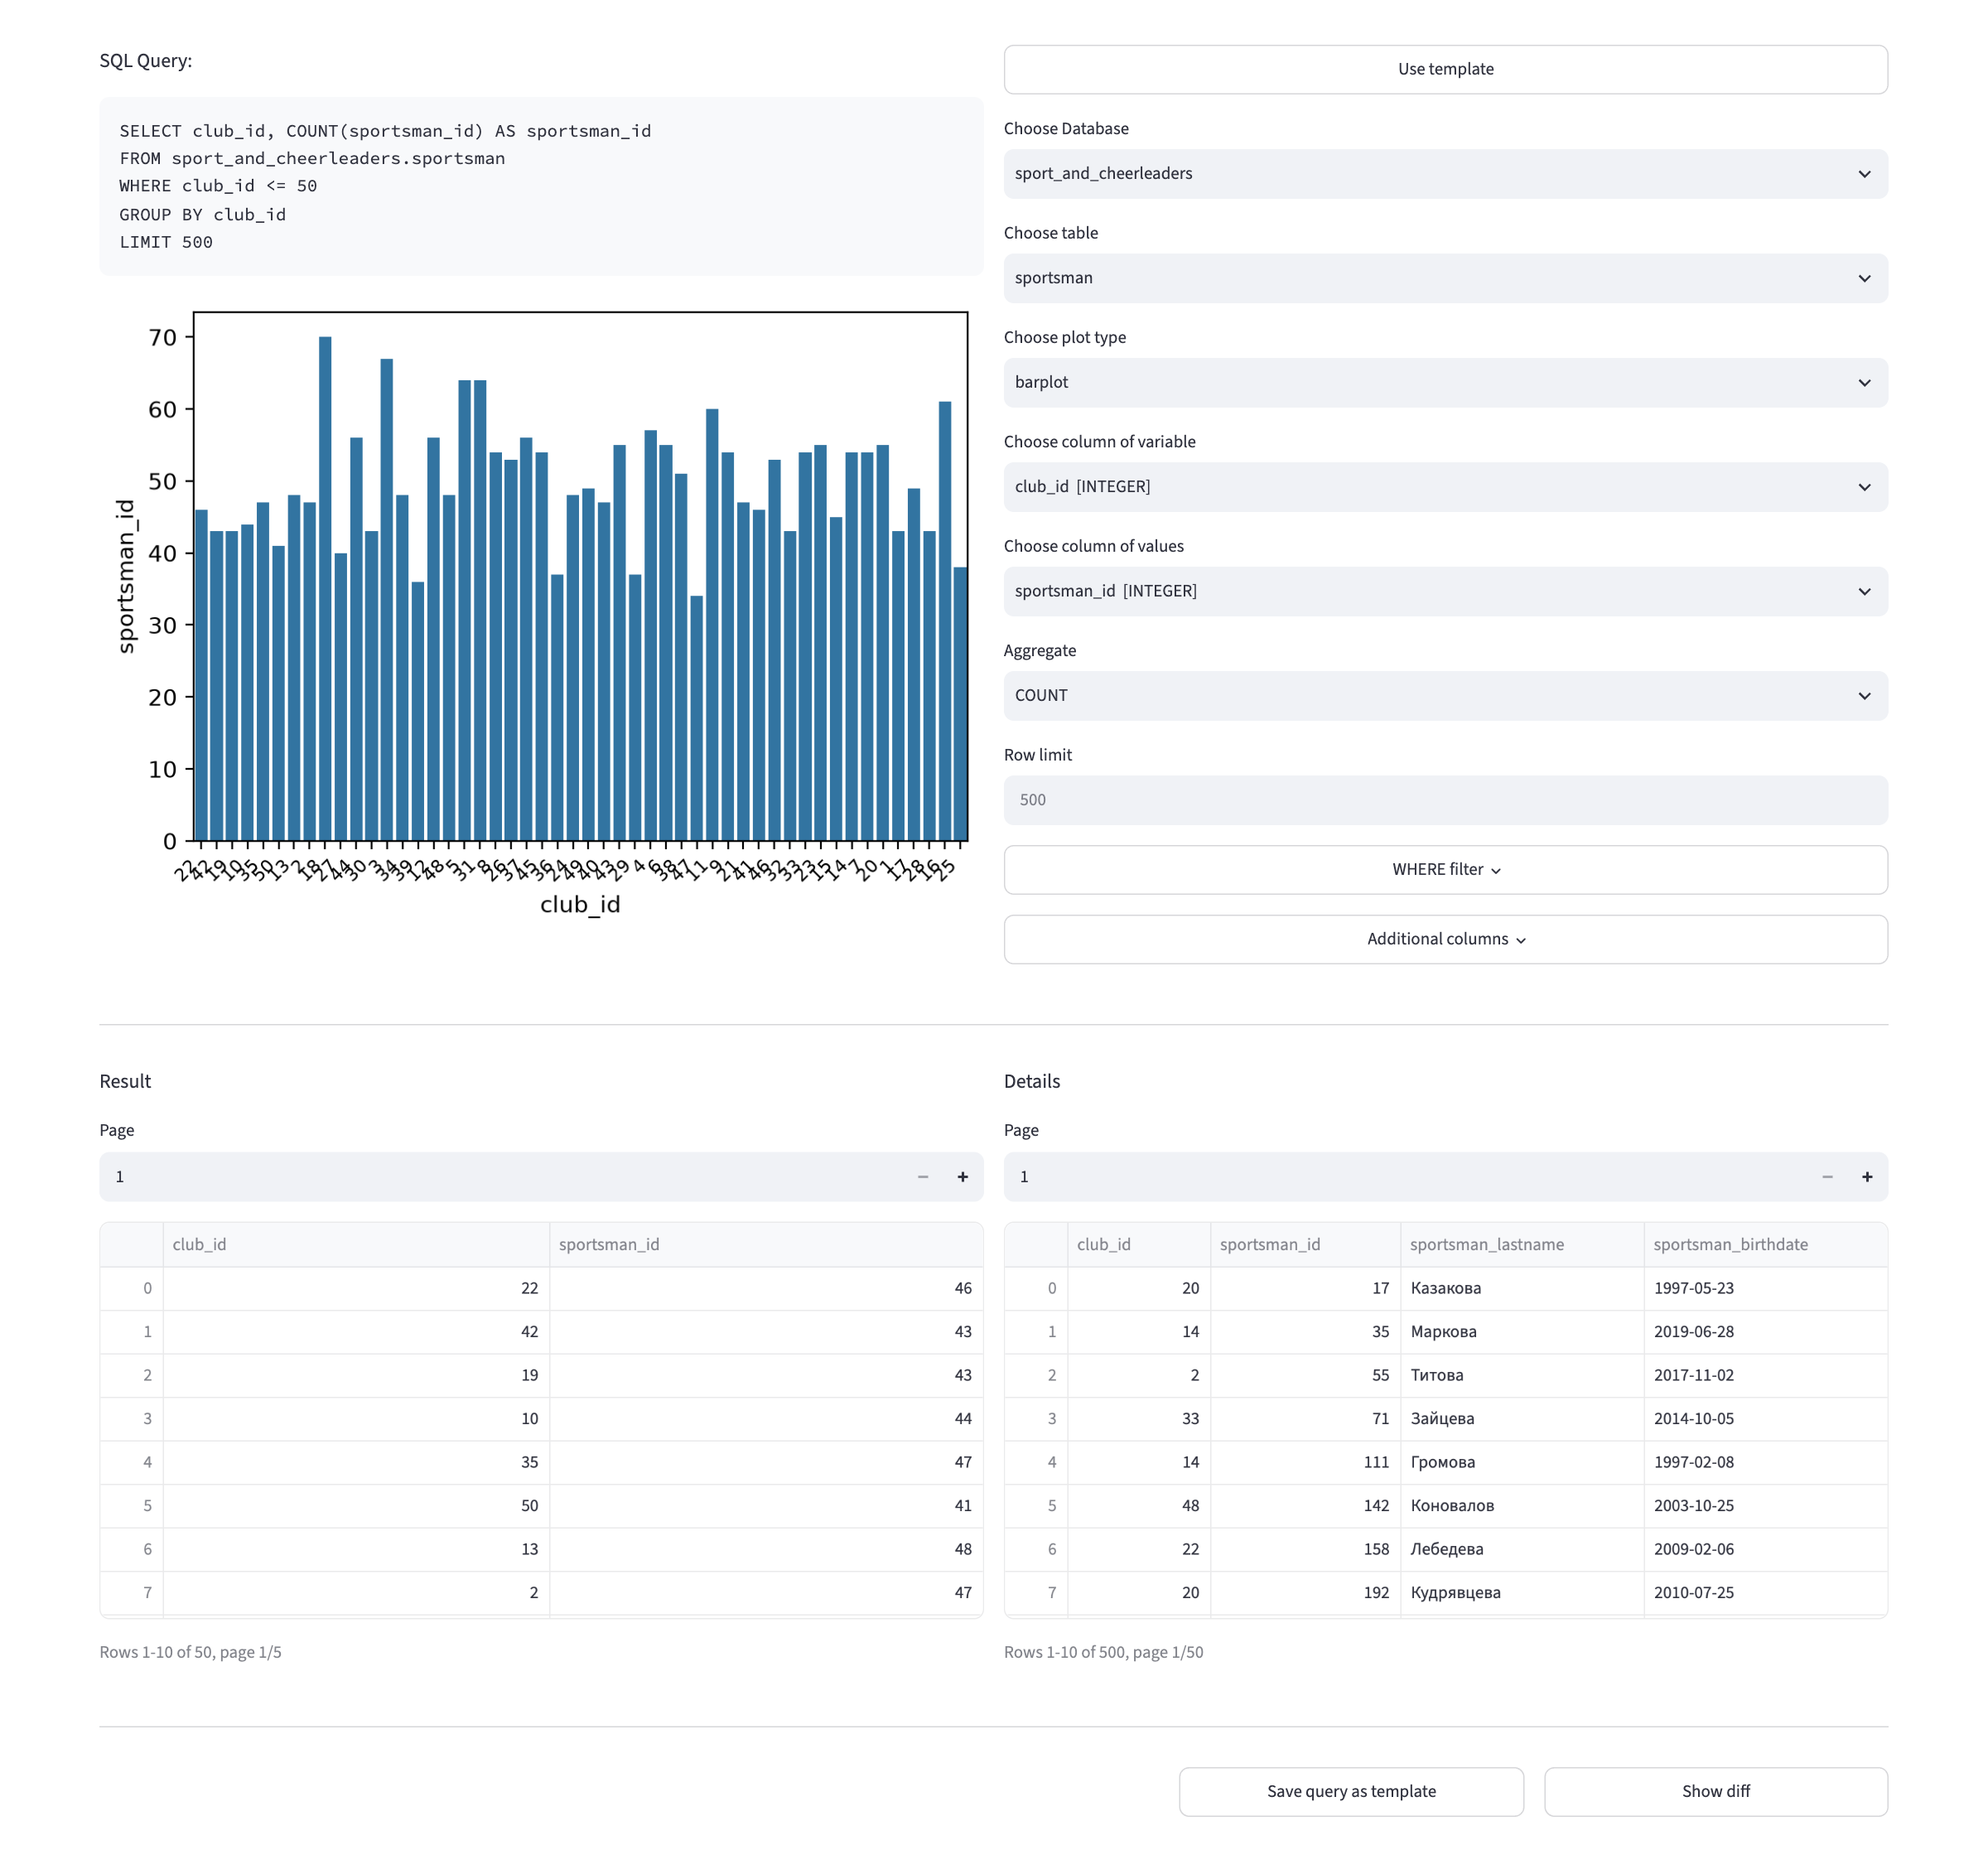
\includegraphics[width=\linewidth]{img/SCEN_7.png}
    \caption{Сценарий 7}
    \label{fig:scen7}
\end{figure}

\subsection{Сценарий 8}
Вывод среднего опыта репетиторов AVG(experience) по городам city\_id из таблицы tutors базы extra\_for\_students, где опыт experience $\geq$ 5 лет.
Итоговый SQL запрос приведен в листинге \ref{lis:scen8}, результат на рисунке \ref{fig:scen8}.
\begin{lstlisting}[language=SQL, caption={Сценарий 8: итоговый SQL запрос}, label={lis:scen8}]
SELECT city_id, AVG(experience) AS experience
FROM extra_for_students.tutors
WHERE experience >= 5
GROUP BY city_id
LIMIT 500
\end{lstlisting}
\begin{figure}[H]
    \center
    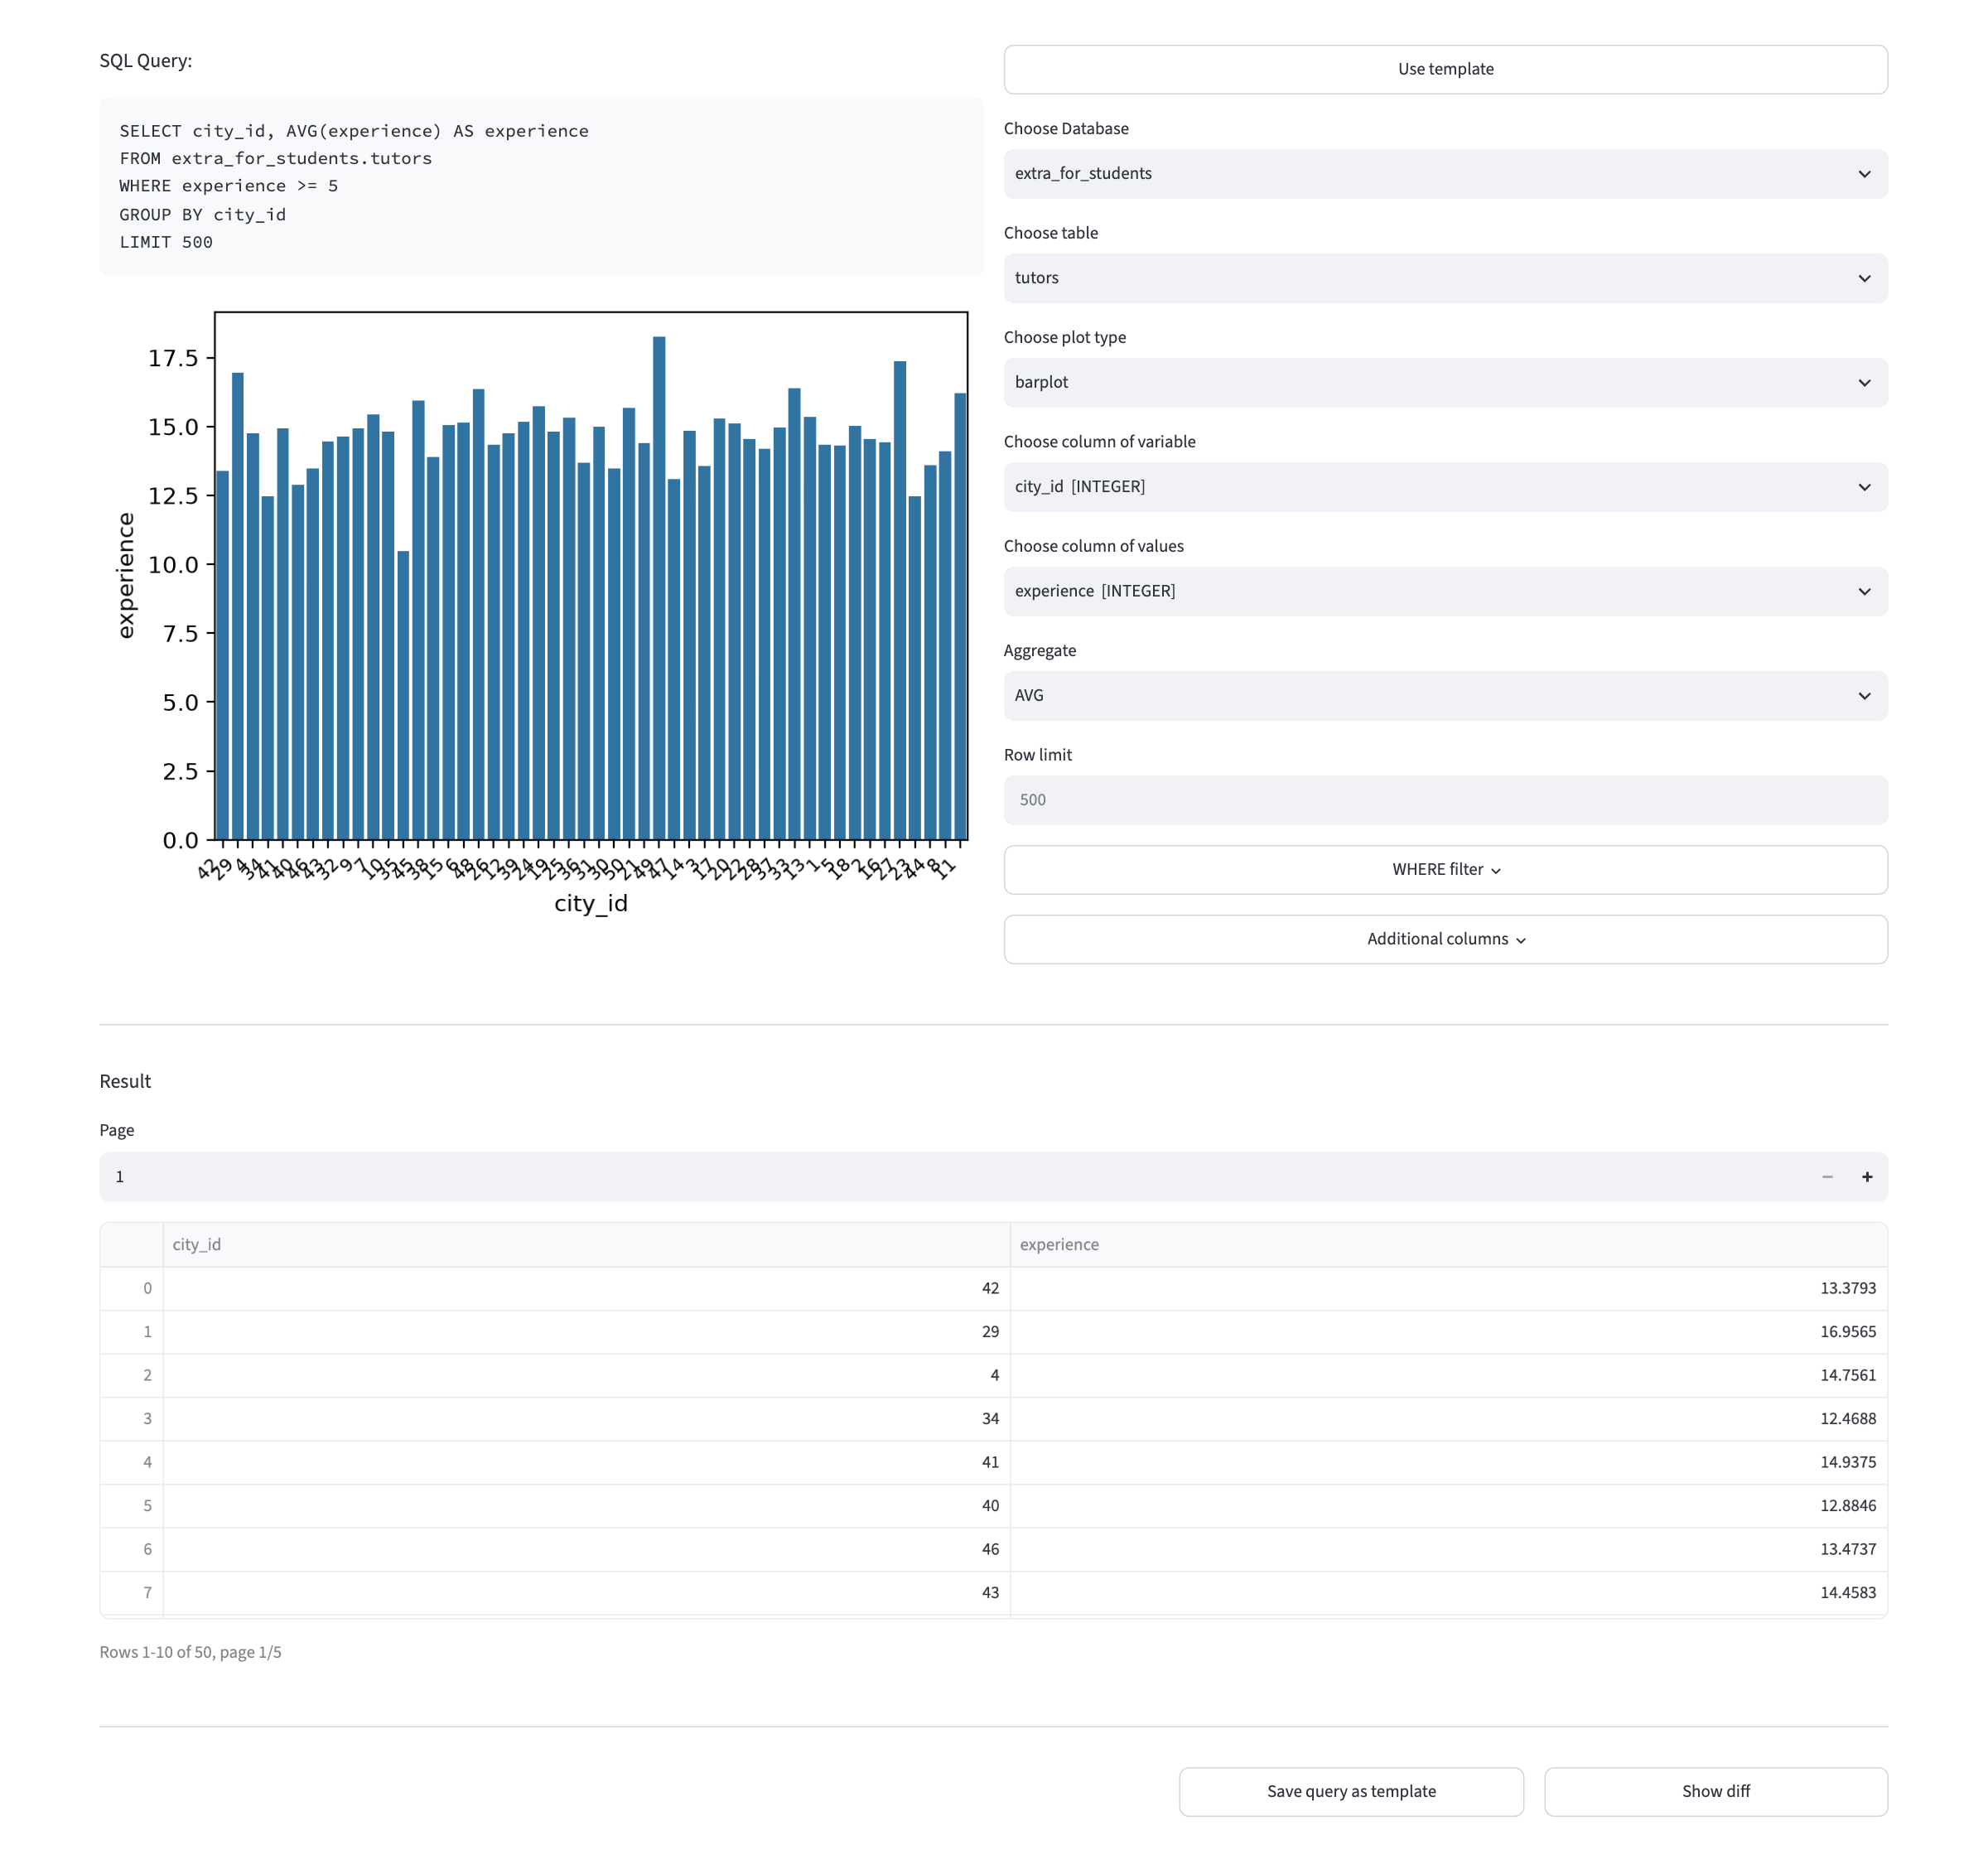
\includegraphics[width=\linewidth]{img/SCEN_8.png}
    \caption{Сценарий 8}
    \label{fig:scen8}
\end{figure}

\subsection{Сценарий 9}
Вывод суммарного числа спортсменов-призеров SUM(sportsman\_count) по занятым местам perfomance\_place из таблицы perfomance базы sport\_and\_cheerleaders, где perfomance\_place $\leq$ 3.
Итоговый SQL запрос приведен в листинге \ref{lis:scen9}, результат на рисунке \ref{fig:scen9}.
\begin{lstlisting}[language=SQL, caption={Сценарий 9: итоговый SQL запрос}, label={lis:scen9}]
SELECT perfomance_place, SUM(sportsman_count) AS sportsman_count
FROM sport_and_cheerleaders.perfomance
WHERE perfomance_place <= 3
GROUP BY perfomance_place
LIMIT 500
\end{lstlisting}
\begin{figure}[H]
    \center
    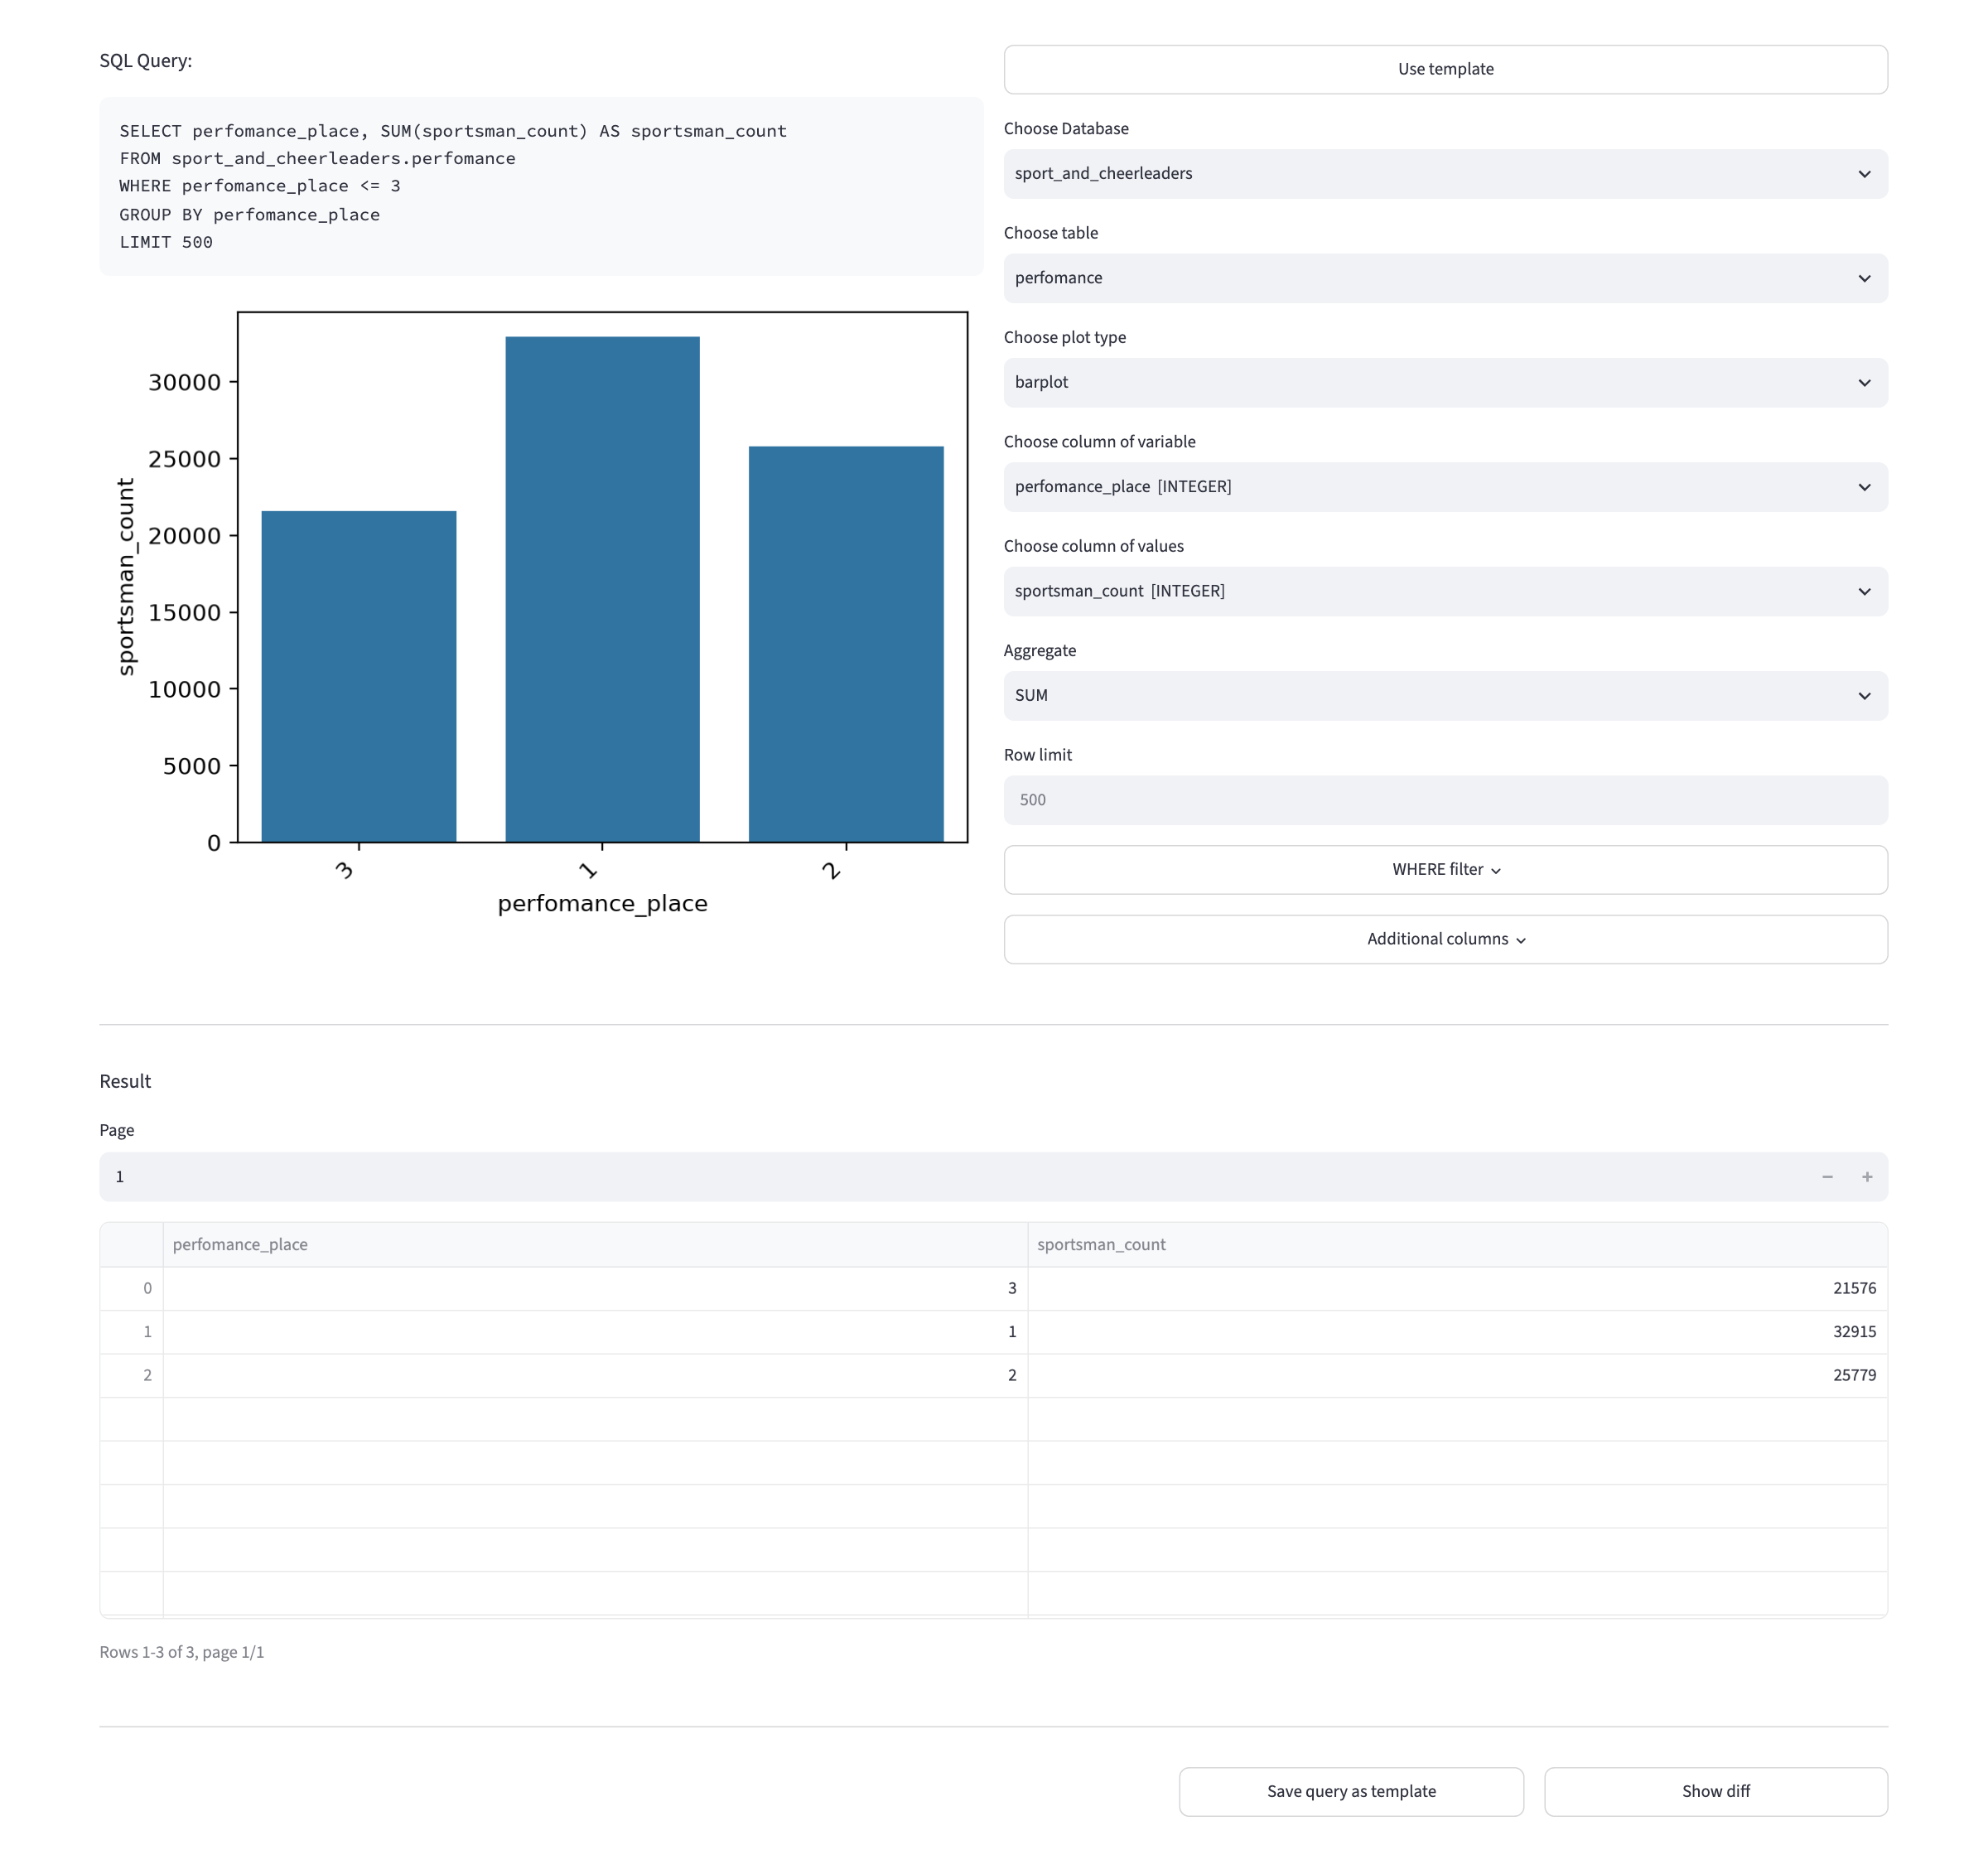
\includegraphics[width=\linewidth]{img/SCEN_9.png}
    \caption{Сценарий 9}
    \label{fig:scen9}
\end{figure}

\subsection{Сценарий 10}
Вывод количества результатов COUNT(result\_id) по итогам выступления attempt\_id (финишировал, DNF, DSQ, DNS) из таблицы result базы mountain\_sport.
Итоговый SQL запрос приведен в листинге \ref{lis:scen10}, результат на рисунке \ref{fig:scen10}.
\begin{lstlisting}[language=SQL, caption={Сценарий 10: итоговый SQL запрос}, label={lis:scen10}]
SELECT attempt_id, COUNT(result_id) AS result_id
FROM mountain_sport.result
GROUP BY attempt_id
LIMIT 500
\end{lstlisting}
\begin{figure}[H]
    \center
    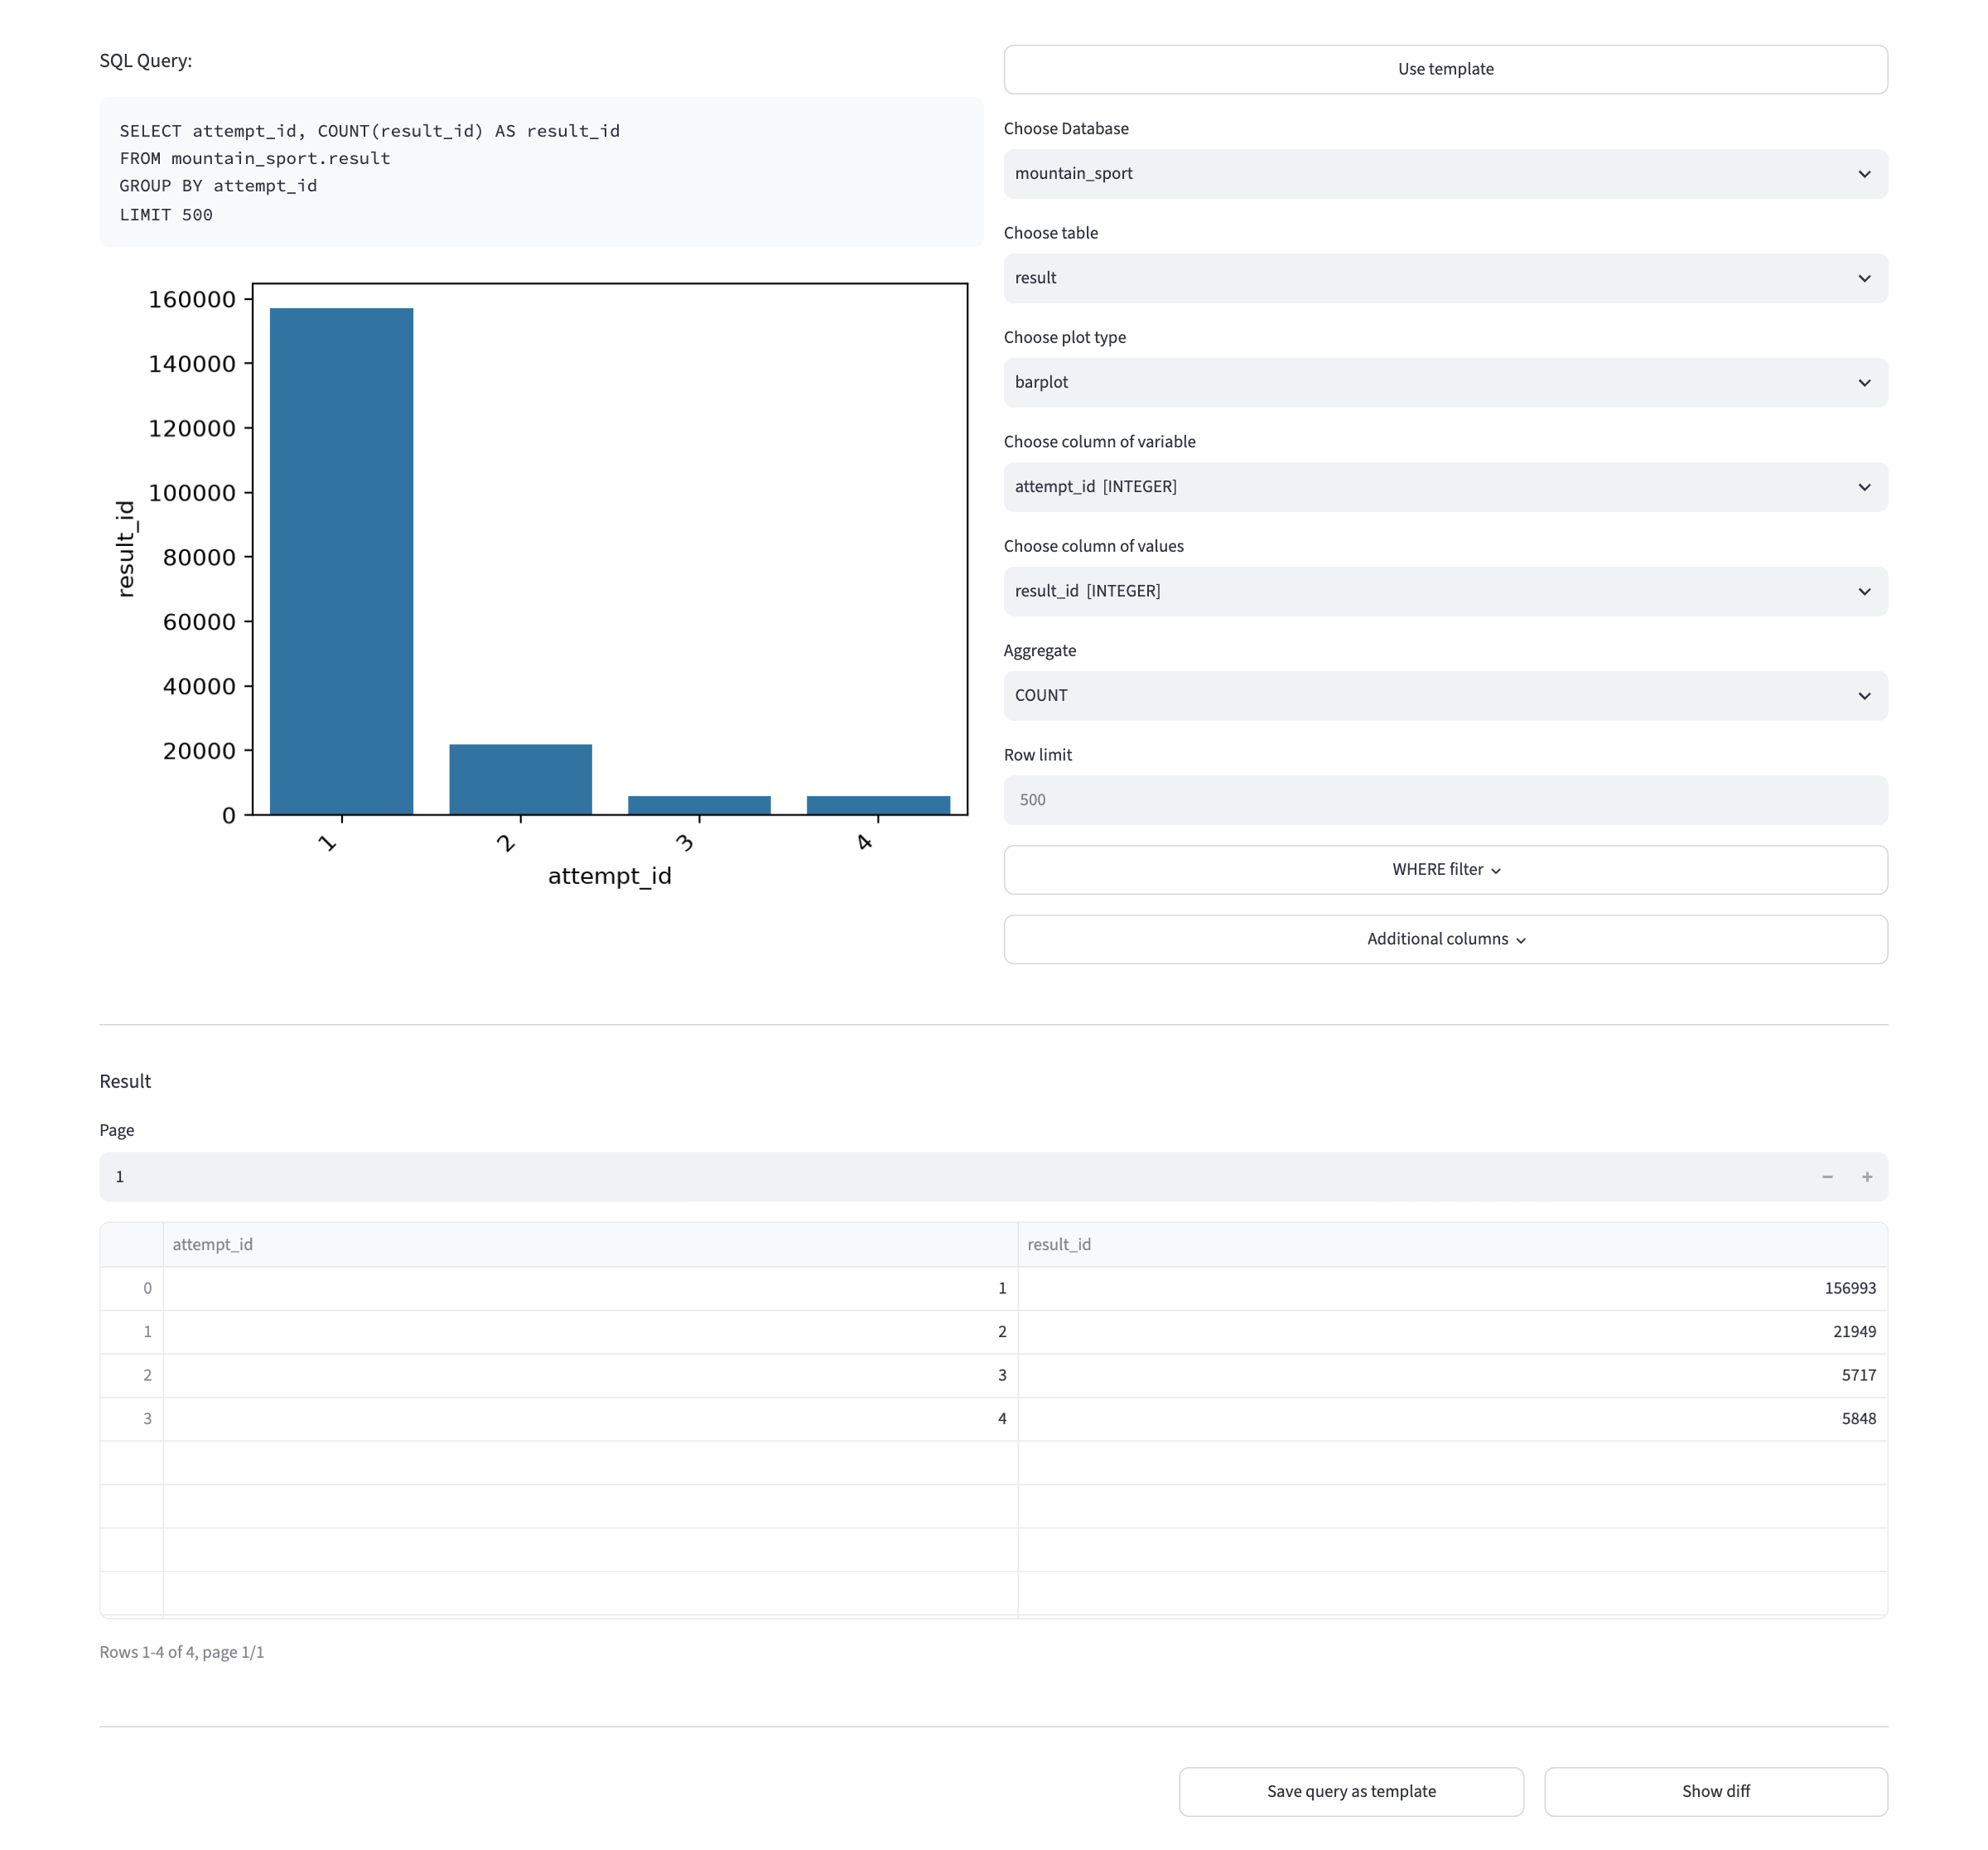
\includegraphics[width=\linewidth]{img/SCEN_10.png}
    \caption{Сценарий 10}
    \label{fig:scen10}
\end{figure}

\subsection{Сценарий 11}
Вывод среднего лучшего времени первой попытки AVG(attempt1\_result) по дисциплинам discipline из таблицы competition базы mountain\_sport, где attempt1\_result $>$ 0.
Итоговый SQL запрос приведен в листинге \ref{lis:scen11}, результат на рисунке \ref{fig:scen11}.
\begin{lstlisting}[language=SQL, caption={Сценарий 11: итоговый SQL запрос}, label={lis:scen11}]
SELECT discipline, AVG(attempt1_result) AS attempt1_result
FROM mountain_sport.competition
WHERE attempt1_result > 0
GROUP BY discipline
LIMIT 500
\end{lstlisting}
\begin{figure}[H]
    \center
    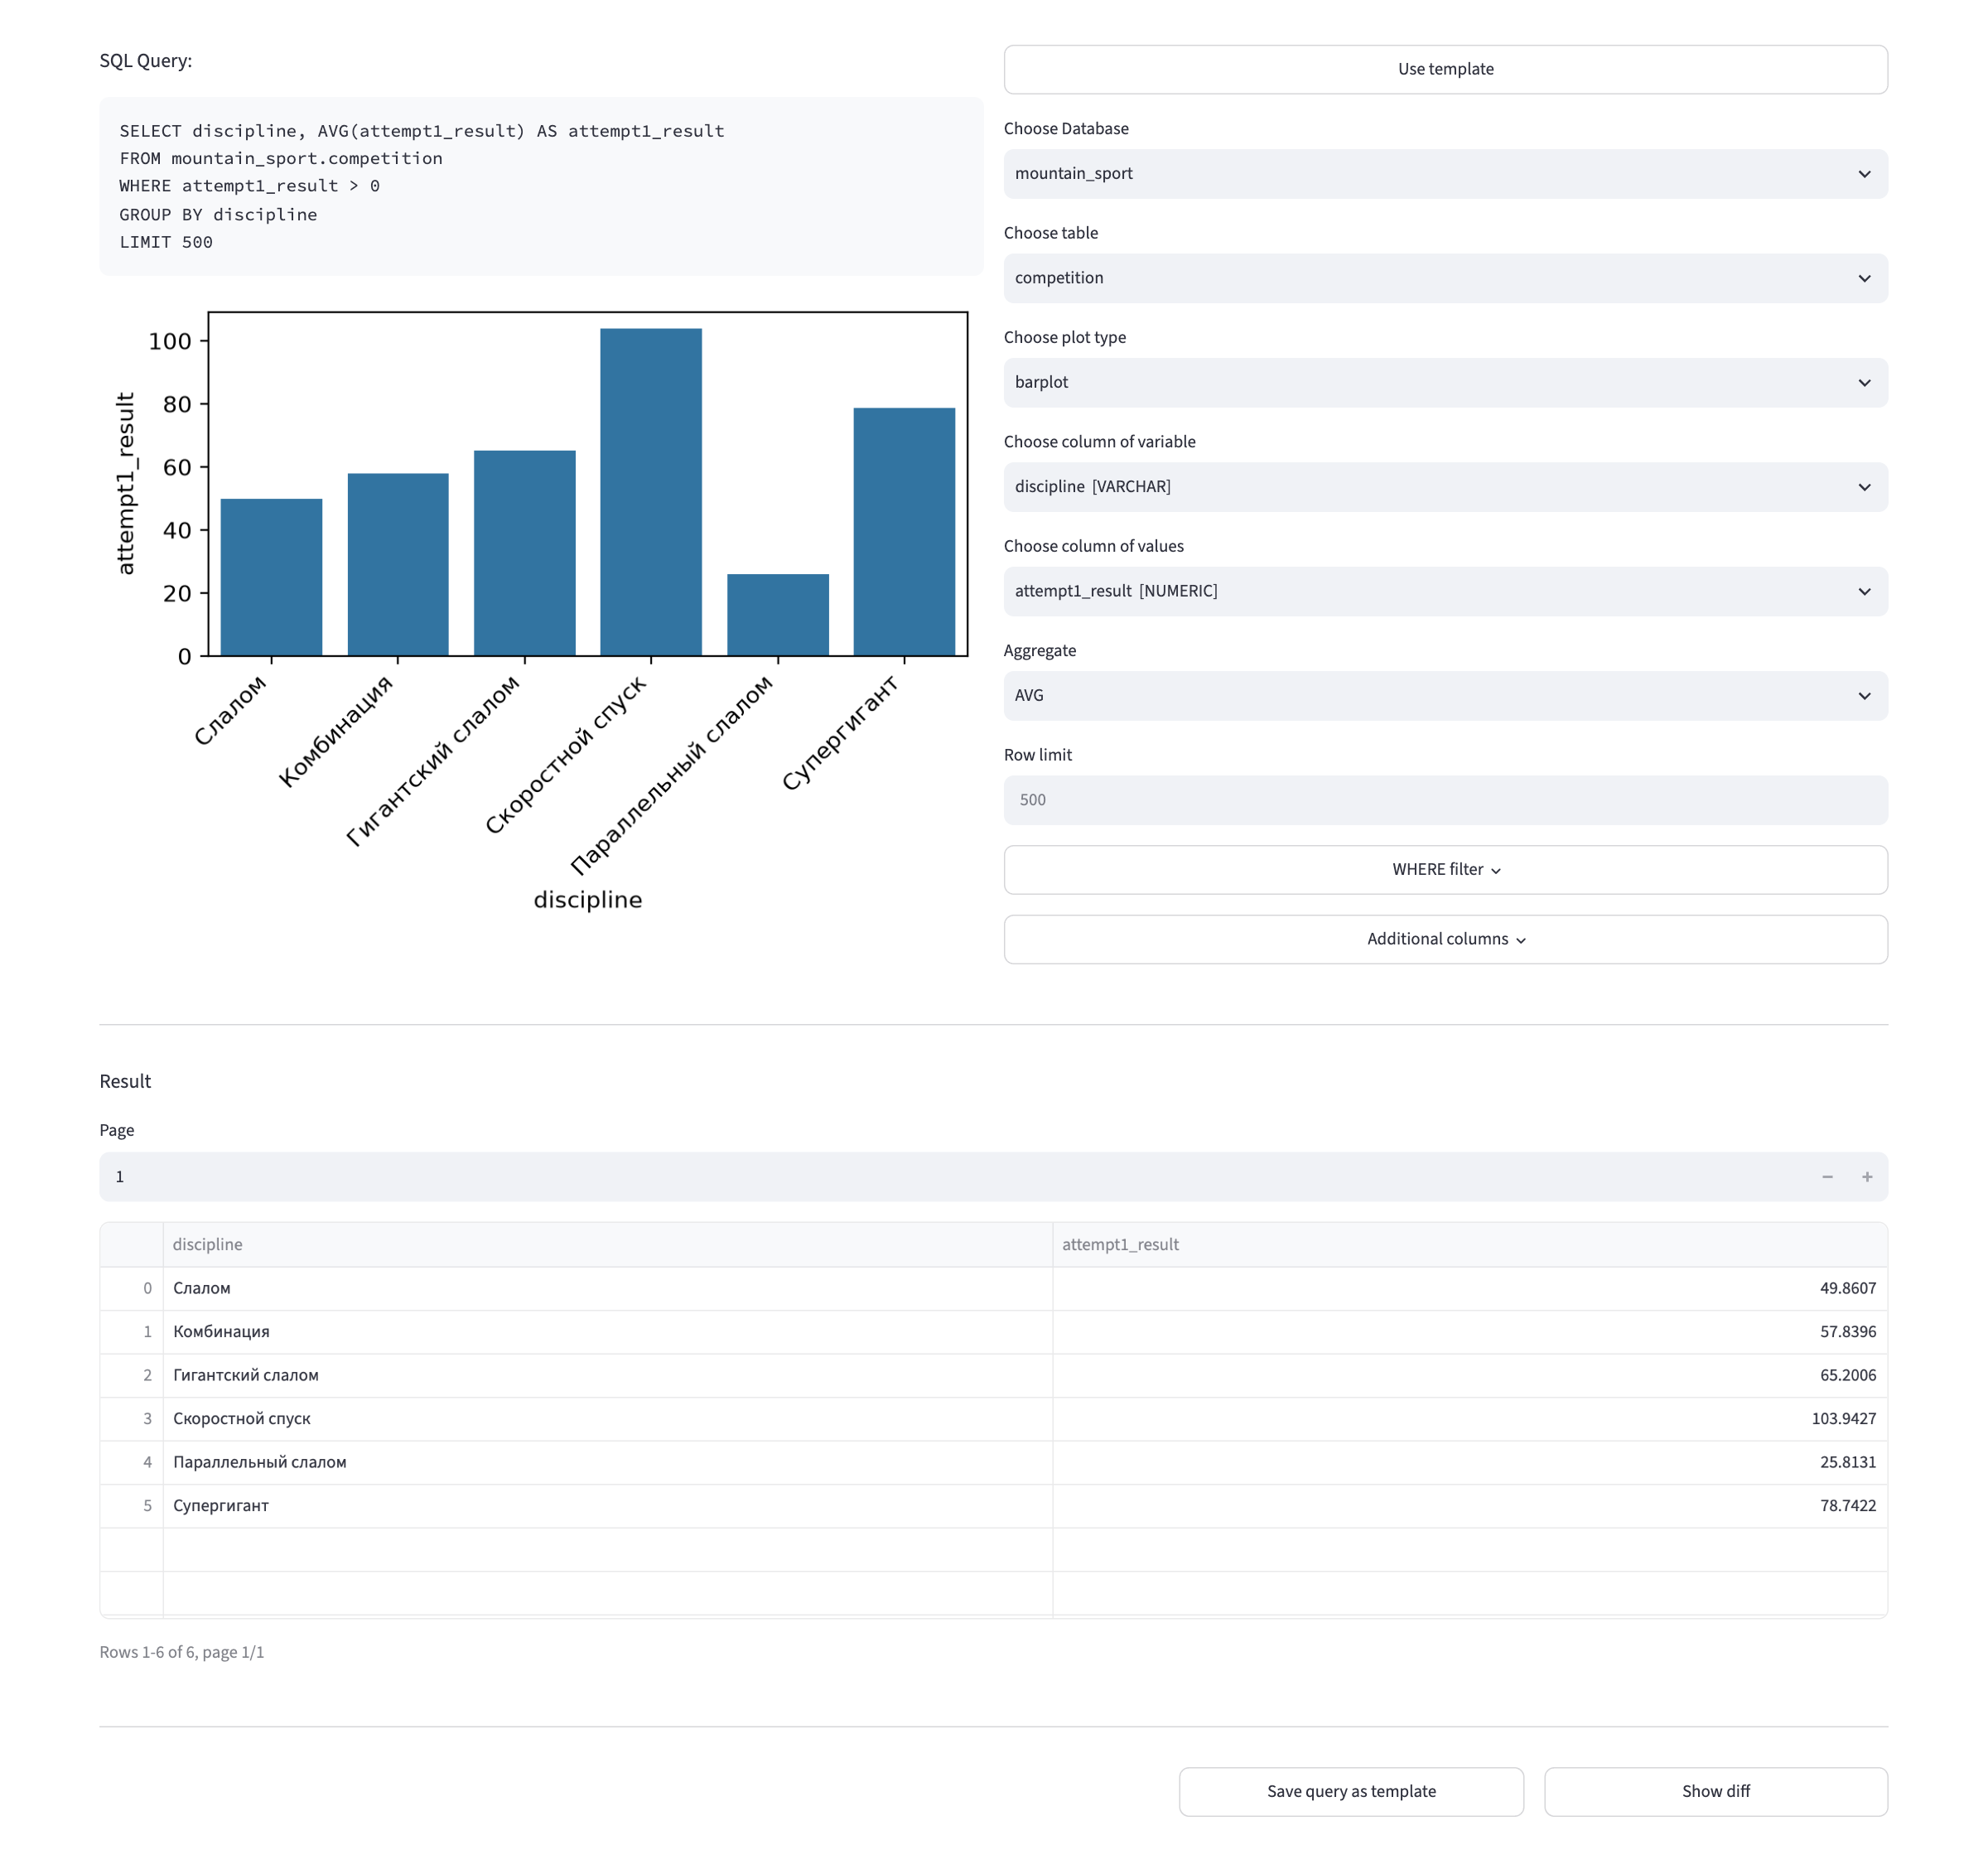
\includegraphics[width=\linewidth]{img/SCEN_11.png}
    \caption{Сценарий 11}
    \label{fig:scen11}
\end{figure}

\newpage
\section*{Заключение}
\addcontentsline{toc}{section}{Заключение}

В ходе работы была спроектирована и реализована система, работающая с метаданными независимых баз данных в единой СУБД postgres.
Развернуты три базы данных источников (учет репетиторов, горнолыжные соревнования, чирлидинг), заполненные сгенерированными данными,
отдельная база метаданных с денормализованным аналогом информационной схемы meta.catalog и отдельная база шаблонов SQL запросов.
Каждая база работает в собственном Docker контейнере со своим томом и изолированной сетью, а взаимодействие между базами выполняется через REST API.

Разработан интерфейс на Streamlit, в котором запрос к источнику собирается из форм по данным каталога метаданных:
выбор базы, таблицы, колонок и агрегатной функции (SUM, AVG, COUNT), ограничение количества строк, вывод SQL запроса, таблиц результата и графика.
Реализованы сохранение и повторное использование шаблонов запросов, сравнение двух шаблонов между собой,
а так же просмотр отличий каталога от реальной схемы источника с возможностью обновления до текущего состояния.

Дополнительно к столбчатой диаграмме были реализованы круговая диаграмма (pieplot), диаграмма рассеивания (scatterplot) и тепловая карта (heatmap),
форма условий WHERE с операторами сравнения для числовых колонок и поиском через LIKE для строковых,
а так же вывод дополнительных колонок исходной таблицы.

В результате получилась минимальная BI система, позволяющая без написания SQL вручную выбирать данные из независимых источников,
агрегировать и фильтровать их, визуализировать в виде графиков, сохранять запросы как шаблоны и отслеживать изменения структуры источников.

\newpage
\section*{Список источников}
\addcontentsline{toc}{section}{Список источников}
\begin{enumerate}
    \item Chapter 35. The information schema. Postgresql [Электронный ресурс], URL: \url{https://www.postgresql.org/docs/current/information-schema.html}, дата обращения (23.09.2026).
    \item Tableau Help. Tableau [Электронный ресурс], URL: \url{https://www.tableau.com/support/help}, дата обращения (25.09.2026).
    \item PostgreSQL Metadata. IBM [Электронный ресурс], URL: \url{https://www.ibm.com/docs/en/streamsets-legacy-dc/5.12.0?topic=processors-postgresql-metadata}, дата обращения (23.09.2026).
\end{enumerate}
\end{document}